\documentclass[14pt, a4paper, oneside]{extarticle}
\usepackage[utf8]{inputenc}
\usepackage[english, russian]{babel}
\usepackage[T1, T2A]{fontenc}
\usepackage{titlesec}
\usepackage{hyperref}
\usepackage[left=3cm,right=2cm,top=2cm,bottom=2cm,bindingoffset=0cm]{geometry}
\usepackage{indentfirst}
\usepackage{graphicx}
\usepackage{enumitem}
\usepackage{array}
\usepackage[justification=centering]{caption}
\usepackage{float}
\usepackage{lscape}
\usepackage{tikz}
\graphicspath{ {./images/} }
\tolerance=10000 % разреженность строки
\linespread{1.4} % интерлиньяж
\hypersetup{
    colorlinks=true,
    linkcolor=black,
    urlcolor=black,
    citecolor=black,
}
\newcommand{\ExternalLink}{
    \tikz[x=1.2ex, y=1.2ex, baseline=-0.05ex]{
        \begin{scope}[x=1ex, y=1ex]
            \clip (-0.1,-0.1) 
                --++ (-0, 1.2) 
                --++ (0.6, 0) 
                --++ (0, -0.6) 
                --++ (0.6, 0) 
                --++ (0, -1);
            \path[draw, 
                line width = 0.5, 
                rounded corners=0.5] 
                (0,0) rectangle (1,1);
        \end{scope}
        \path[draw, line width = 0.5] (0.5, 0.5) 
            -- (1, 1);
        \path[draw, line width = 0.5] (0.6, 1) 
            -- (1, 1) -- (1, 0.6);
        }
    }

\title{Masters Term Paper}
\author{Evgenia Abdullaeva}
\date{May 2022}

\begin{document}
\begin{titlepage}
    \centering
        \begin{figure}[H]
            \centering
            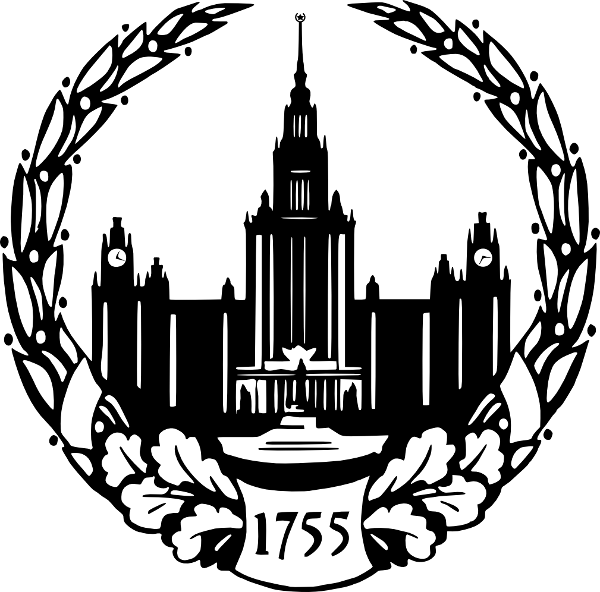
\includegraphics[scale=1.6]{msu-logo}
        \end{figure}
        Московский государственный университет имени М.В. Ломоносова\\
        \vspace{0.5cm}
        Факультет космических исследований\\
        Магистерская программа <<Методы и технологии дистанционного зондирования Земли>>\\
        \vfill
        \textbf{КУРСОВАЯ РАБОТА\\
        на тему: <<Развитие методов классификации и оценки значимости признаков на основе случайных лесов в контексте задачи картографирования земного покрова России>>}\\
        \vfill
        Абдуллаева Евгения Гасановна\\
        \vspace{0.5cm}
        Научный руководитель:\\
        к.т.н. Хвостиков Сергей Антонович
        \vfill
        Москва, 2022 г.
\end{titlepage}

\begin{abstract}
% TODO Аннотация на английском + презентация для английского
\end{abstract}
\selectlanguage{english}
\begin{abstract}

\end{abstract}
\selectlanguage{russian}
\setcounter{page}{2}
\newpage

\tableofcontents
\newpage

\section{Введение}
% Постановка проблемы, цель работы
% TODO

% СМЫСЛ \\
% Зачем классифицировать земной покров? \\
% Зачем новые методы автоматизации классификации земного покрова? \\
% Об алгоритме LAGMA \\
% Что-то о машинном обучении в применении к колоссальным объемам спутниковых данных \\

% Ссылки на [2] и [3]

% % Актуальность
% Ранее к этому набору данных случайные леса не применялись всерьез. Соответственно развитие заключается в применении нового метода классификации, оценке влияния разных параметров/подходов на точность классификации, а также в анализе входных данных, их значимости.

\newpage

\section{Анализ данных}
\subsection{Источник данных}
В данной работе классификация осуществляется на основе спутниковых данных (стандартного продукта MOD09) 2010 года (весенних, летних и осенних) и 2011 года (зимних), полученных спектрорадиометром Moderate Resolution Imaging Spectroradiometer (MODIS), установленным на спутниках Terra и Aqua. Продукт MOD09 представляет собой данные о спектрально-отражательных характеристиках земной поверхности, для которых была выполнена геопривязка и корректировка на атмосферу. Данные предварительно обработаны для исключения влияния облаков и теней от них путем осреднения значений яркости за сезон, по ним созданы сезонные композиты.

Цитируя монографию \cite{land-cover-mapping-monograph}, укажем, что прибор MODIS разработан для изучения биологических и физических процессов в глобальном масштабе с периодичностью наблюдений в 1-2 дня, в частности, для исследований растительного покрова. MODIS имеет 36 спектральных каналов в диапазоне $\lambda$ = 0.46-14.39 мкм, в том числе информативные для изучения растительности красный ($\lambda$ = 0.62-0.67 мкм) и ближний инфракрасный ($\lambda$ = 0.84-0.88 мкм) каналы с пространственным разрешением 250 м, и ряд каналов с разрешением 500 м, используемых для анализа характеристик растительности и фильтрации облачности. Полоса охвата прибора составляет 2330 км, а покрытие данными измерений всей территории России обеспечивается с периодичностью не реже одного раза в сутки. Таким образом, данные прибора образуют непрерывный однородный архив ежедневных наблюдений в течение более 15 лет, анализ которых может быть эффективно использован для изучения и мониторинга растительного покрова. Данные MODIS успешно используются для создания глобальной карты типов земного покрова.

\subsection{Общие сведения о данных}
Данные для классификации представлены в табличном виде. Полный набор данных содержит 74029669 элементов (строк таблицы). Каждый элемент описан 14-ю признаками (столбцы таблицы), содержащими неотрицательные целочисленные значения:

CLASS (значения от 1 до 23) --- индекс класса элемента выборки;

X (значения от 5820 до 40161), Y (значения от 1429 до 20580) --- координаты элемента выборки (индекс пикселя в растровом изображении, размер пикселя --- 230 метров);

WINTER1 (значения от 0 до 10583), WINTER2 (значения от 0 до 10584) --- яркость композитного изображения за зимний сезон в красном канале (RED, $\lambda$ = 0.62-0.67 мкм) и ближнем инфракрасном канале (NIR, $\lambda$ = 0.84-0.88 мкм), соответственно;

SPRING1 (значения от 1 до 8653) --- яркость композитного изображения за весенний сезон в канале RED;

SPRING2 (значения от 1 до 7018) --- яркость композитного изображения за весенний сезон в канале NIR;

SPRING3 (значения от 1 до 5211) --- яркость композитного изображения за весенний сезон в коротковолновом инфракрасном канале (SWIR, $\lambda$ = 1.63-1.65 мкм);

SUMMER1 (значения от 1 до 8653), SUMMER2 (значения от 1 до 6907), SUMMER3 (значения от 1 до 4923) --- яркость композитного изображения за летний сезон в каналах RED, NIR, SWIR, соответственно;

FALL1 (значения от 1 до 8653), FALL2 (значения от 1 до 6907), FALL3 (значения от 1 до 5280) --- яркость композитного изображения за осенний сезон в каналах RED, NIR, SWIR, соответственно.

Классификация выборки изначально проводилась с помощью алгоритма Locally Adaptive Global Mapping Algorithm (LAGMA), формально описанного в \cite{land-cover-mapping-monograph}, методом максимального правдоподобия. Результаты автоматической классификации были подвергнуты экспертному визуальному анализу.

\subsection{Классифицируемые типы земного покрова}
\subsubsection{Тематические классы земного покрова и их представленность в выборке}
Представленные в наборе данных типы земного покрова включают в себя 19 тематических классов, образующих 5 различных групп земного покрова, описание групп и классов приведено ниже в соответствии с монографией \cite{land-cover-mapping-monograph}:

\begin{enumerate}
    \item Леса:
    \begin{itemize}
        \item[-] Темнохвойные вечнозеленые насаждения (\textit{темнохвойный лес}), в пологе которых не менее 80\% площади крон составляют теневыносливые виды хвойных деревьев, включая ель, пихту и сибирскую сосну (кедр).
        \item[-] Светлохвойные вечнозеленые насаждения (\textit{светлохвойный лес}), в пологе которых не менее 80\% площади крон составляют деревья сосны обыкновенной.
        \item[-] Лиственные насаждения (\textit{лиственный лес}), в пологе которых не менее 80\% площади занимают кроны березы и осины, а также широколиственных пород, включая дуб, липу, ясень, клен, вяз и некоторые другие виды.
        \item[-] Смешанные насаждения с преобладанием хвойных пород (\textit{смешанный лес с преобладанием хвойных}), в которых кроны хвойных деревьев занимают от 60\% до 80\%, а лиственных --- от 20\% до 40\% площади полога.
        \item[-] Смешанные насаждения (\textit{смешанный лес}), в которых площади крон хвойных и лиственных пород деревьев представлены примерно в равных пропорциях (40-60\%) в пологе.
        \item[-] Смешанные насаждения с преобладанием лиственных пород (\textit{смешанный лес с преобладанием лиственных}), в которых кроны лиственных пород деревьев занимают от 60\% до 80\%, а хвойных --- от 20\% до 40\% площади полога.
        \item[-] Хвойные листопадные (лиственничные) насаждения (\textit{хвойный листопадный лес}), в пологе которых кроны деревьев лиственницы занимают более 80\% площади.
        \item[-] \textit{Редины хвойные листопадные} (лиственничные), представляющие собой участки, занятые отдельно стоящими деревьями или разреженными насаждениями лиственницы с проектным покрытием крон менее 20\%.
    \end{itemize}
    \item Травяно-кустарниковая растительность:
    \begin{itemize}
        \item[-] \textit{Луга} --- травяная растительность с продолжительностью вегетационного сезона более 5 месяцев, видовой состав которой характеризуется господством многолетних трав, главным образом злаков и осоковых, в условиях достаточного увлажнения. Площадь проекции крон деревьев и кустарников на земную поверхность составляет менее 20\%.
        \item[-] \textit{Степь} --- травяной покров образован преимущественно засухоустойчивыми 
        многолетними дерновинными злаками (ковыль, типчак, полынь, житняк и др.).Встречается большое разнообразие видов степных кустарников и полукустарников, а также короткоцветущих эфемероидов и эфемеров.
        \item[-] Хвойные вечнозеленые кустарники (\textit{хвойный кустарник}) --- кустарниковые заросли или низкоствольные леса из кедрового стланика.
        \item[-] Лиственные кустарники (\textit{лиственный кустарник}) --- сообщество низкорослых и стелющихся кустарников (кустарниковых или карликовых берез, полярных ив и др.).
    \end{itemize}
    \item Тундра:
    \begin{itemize}
        \item[-] \textit{Кустарничковая тундра} --- сухая тундра с редкой фрагментарной растительностью, среди которой доминируют виды альпоарктических кустарничковых сообществ высотой менее 15 см. Распространены также мохово-лишайниковый покров и разнотравье.
        \item[-] \textit{Травянистая тундра} представлена главным образом различными видами трав и мхов, произрастающими на сырых почвах и образующими сплошной растительный покров. Часто встречаются кустарнички высотой до 40 см.
        \item[-] \textit{Кустарниковая тундра} с доминированием кустарников (карликовая береза и различные виды ивы) высотой более 40 см, иногда с примесью можжевельника, ольхи или кедрового стланика.
    \end{itemize}
    \item Водно-болотные комплексы:
    \begin{itemize}
        \item[-] \textit{Болота} --- территории, характеризующиеся избыточным увлажнением с преобладанием растительного покрова из мхов, лишайников, тростника, осоки и некоторых других видов. Часто встречаются участки с наличием редкого (<20\%) древесного полога.
        \item[-] \textit{Прибрежная растительность} --- гидрофильная травяная и древеснокустарниковая растительность по берегам водоемов, часто периодически затопляемая.
    \end{itemize}
    \item Не покрытые растительностью земли:
    \begin{itemize}
        \item[-] \textit{Открытые грунты и выходы горных пород} --- земли, суммарное проективное покрытые которых растительностью всех видов не превышает 20\%.
        \item[-] \textit{Водные объекты} --- речные и озерные внутренние водоемы, а также прибрежные участки открытой воды.
    \end{itemize}
\end{enumerate}

\begin{table}[H]
    \centering
    \caption{Количество представителей тематических классов\\земного покрова в выборке}
    \begin{tabular}{ m{12.1cm}r }
        \textbf{Класс} & \textbf{Количество} \\
        \hline
        Темнохвойный лес & 6153034 \\
        Светлохвойный лес & 4500884 \\
        Лиственный лес & 8734036 \\
        Смешанный лес с преобладанием хвойных & 1025492 \\
        Смешанный лес & 378946 \\
        Смешанный лес с преобладанием лиственных & 1505855 \\
        Хвойный листопадный лес & 22271771 \\
        Редины хвойные листопадные & 3586296 \\
        Луга & 5858059 \\
        Степь & 2091630 \\
        Хвойный кустарник & 1096112 \\
        Лиственный кустарник & 267236 \\
        Кустарничковая тундра & 1943579 \\
        Травянистая тундра & 4893560 \\
        Кустарниковая тундра & 1178381 \\
        Болота & 4657062 \\
        Прибрежная растительность & 9661 \\
        Открытые грунты и выходы горных пород & 2691471 \\
        Водные объекты & 1186604 \\
        \hline
        Всего элементов & 74029669 \\
    \end{tabular}
\end{table}

\begin{figure}[H]
    \caption{Относительное количество представителей тематических классов земного покрова в выборке}
    \centering
    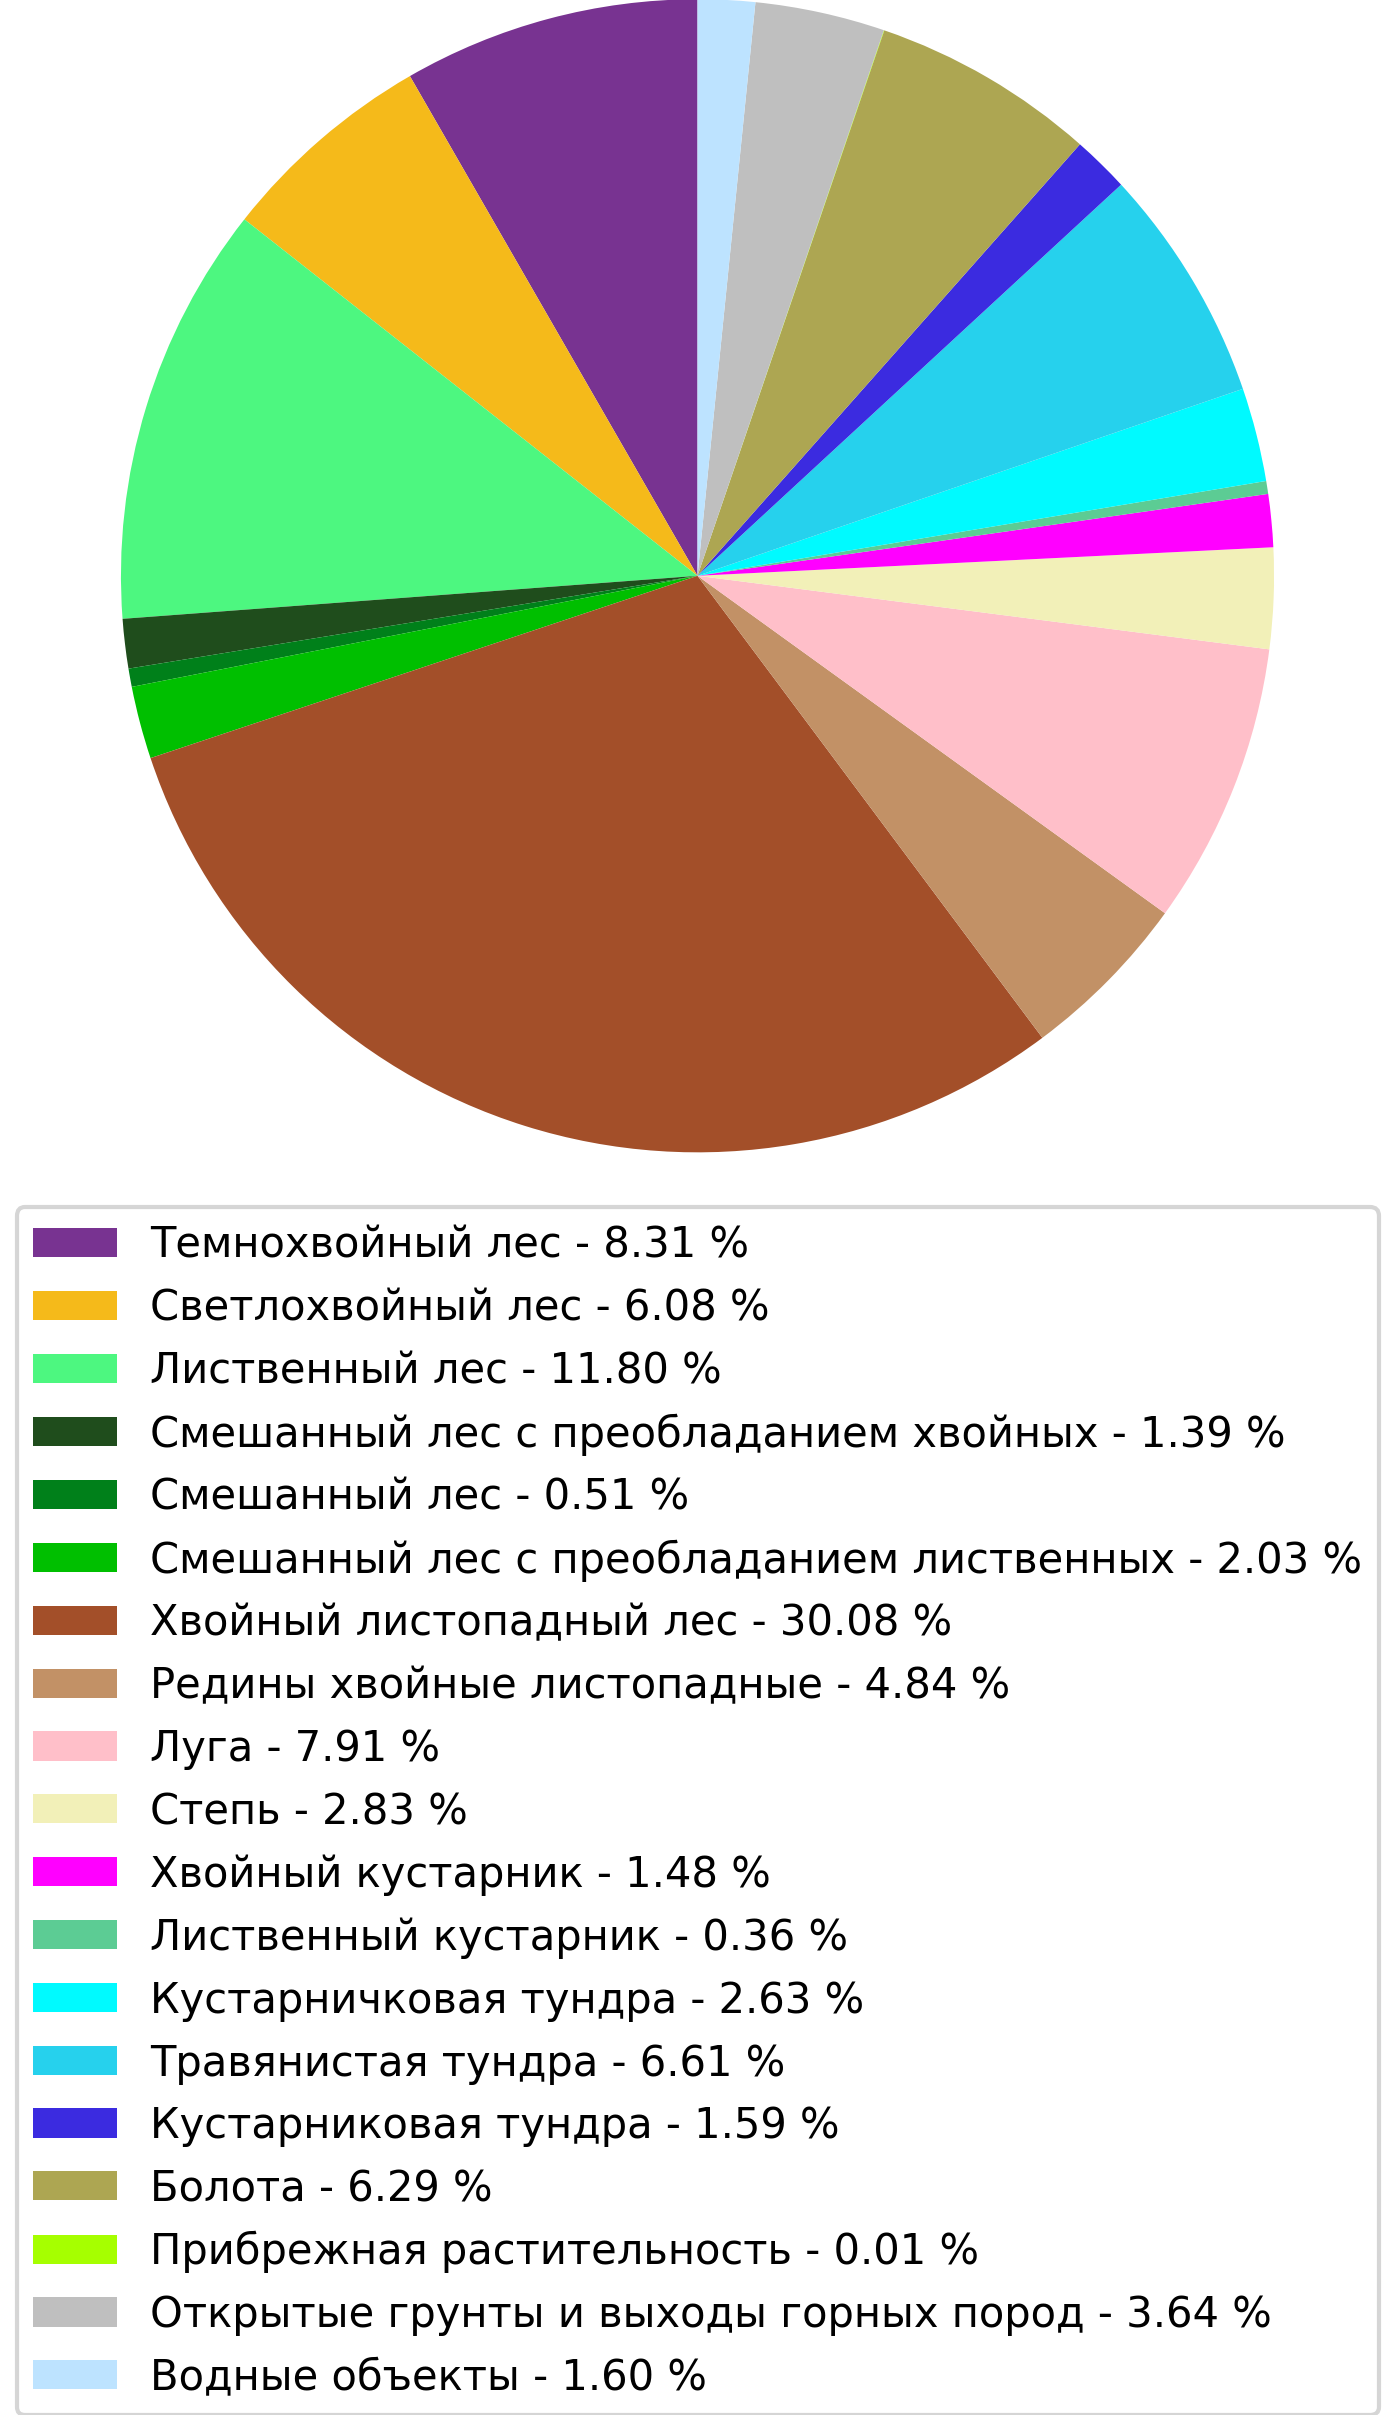
\includegraphics[scale=0.8]{classes-ratio}
\end{figure}

\subsubsection{Визуализация тематических классов земного покрова}
\begin{figure}[H]
    \caption{Визуализация тематических классов земного покрова, представленных в выборке. Для каждого класса на первом графике представлена диаграмма размаха, показывающая медиану, нижний и верхний квантили, минимальное и максимальное значение сезонной яркости в различных спектральных каналах; на втором графике представлена карта пространственного распределения элементов-представителей класса (синим).}
\end{figure}

\begin{figure}[H]
    \centering
    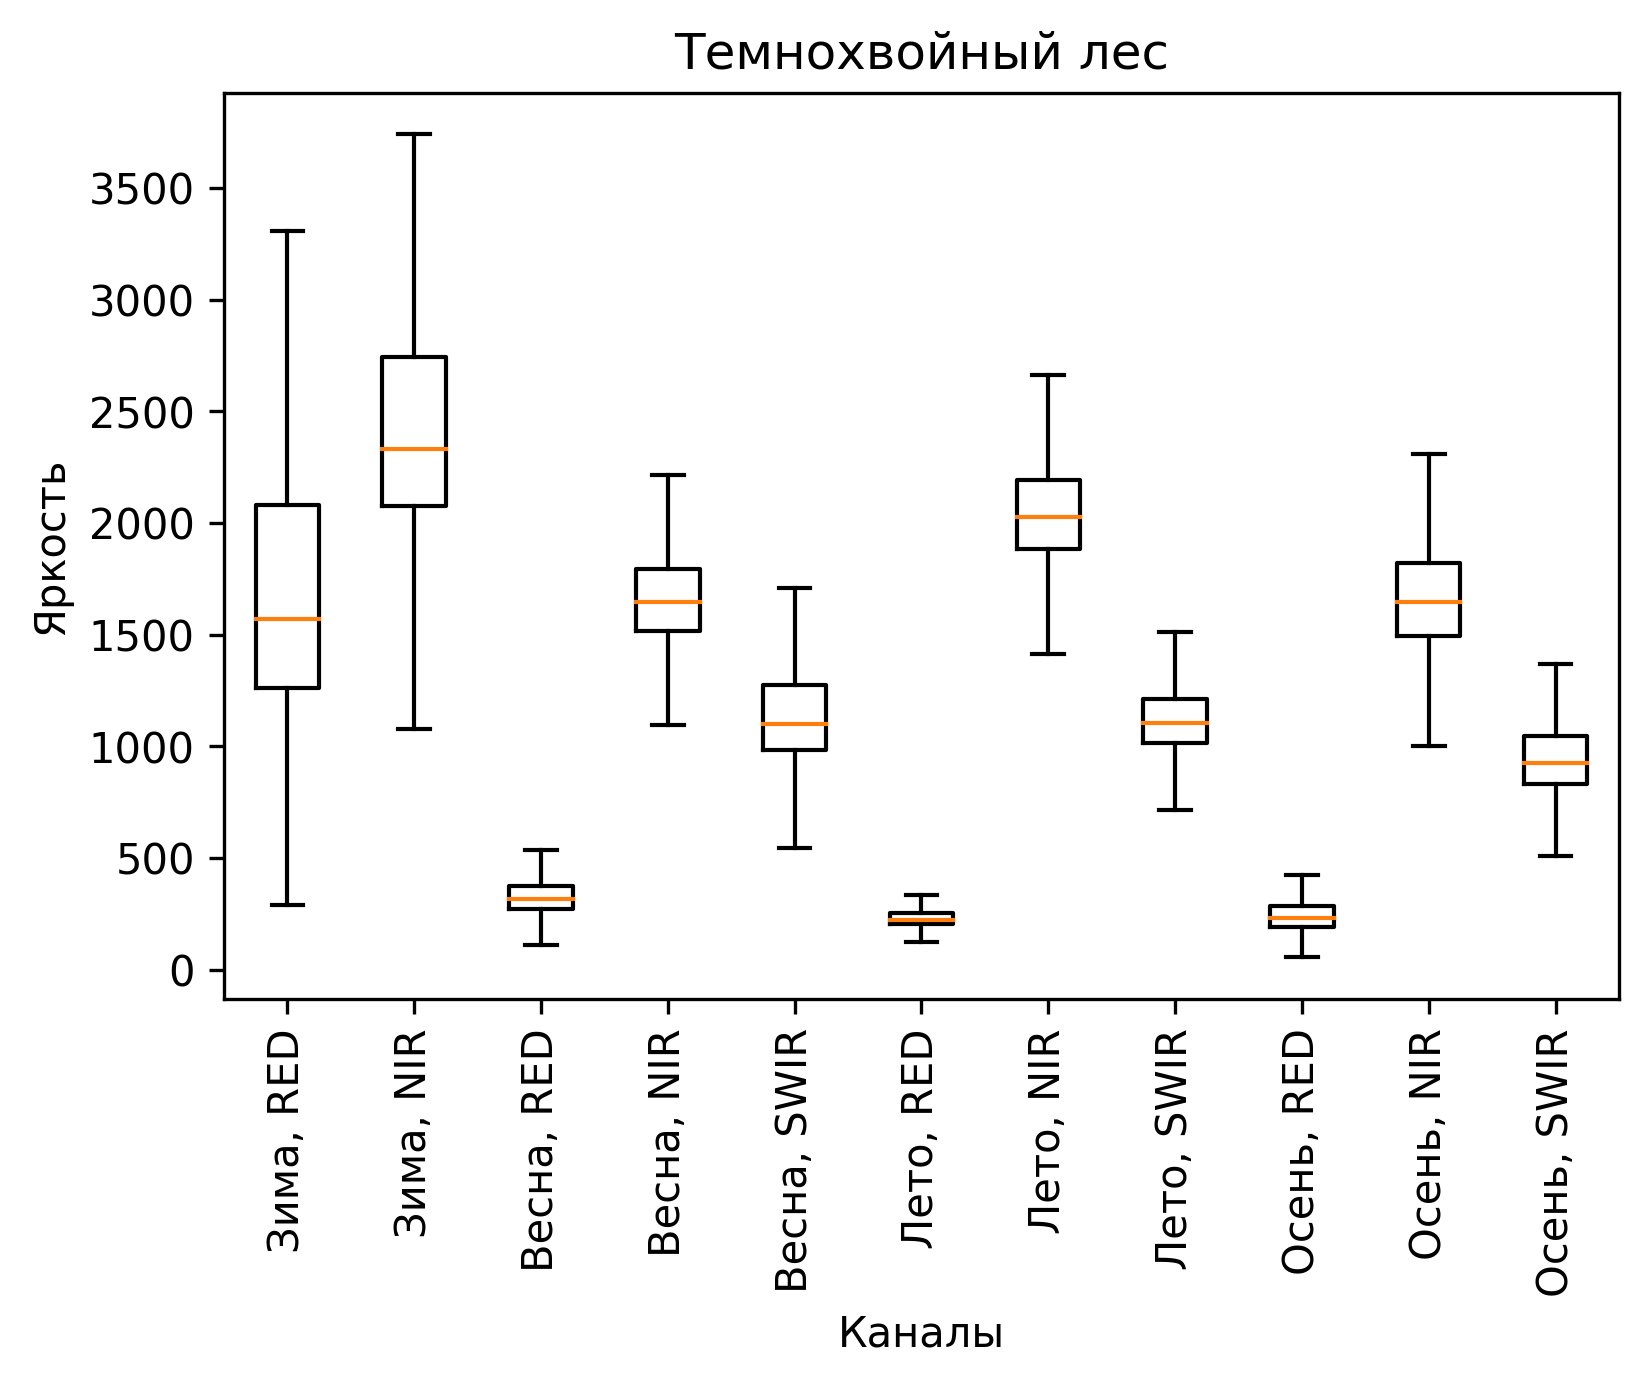
\includegraphics[]{class-1-boxplot}
    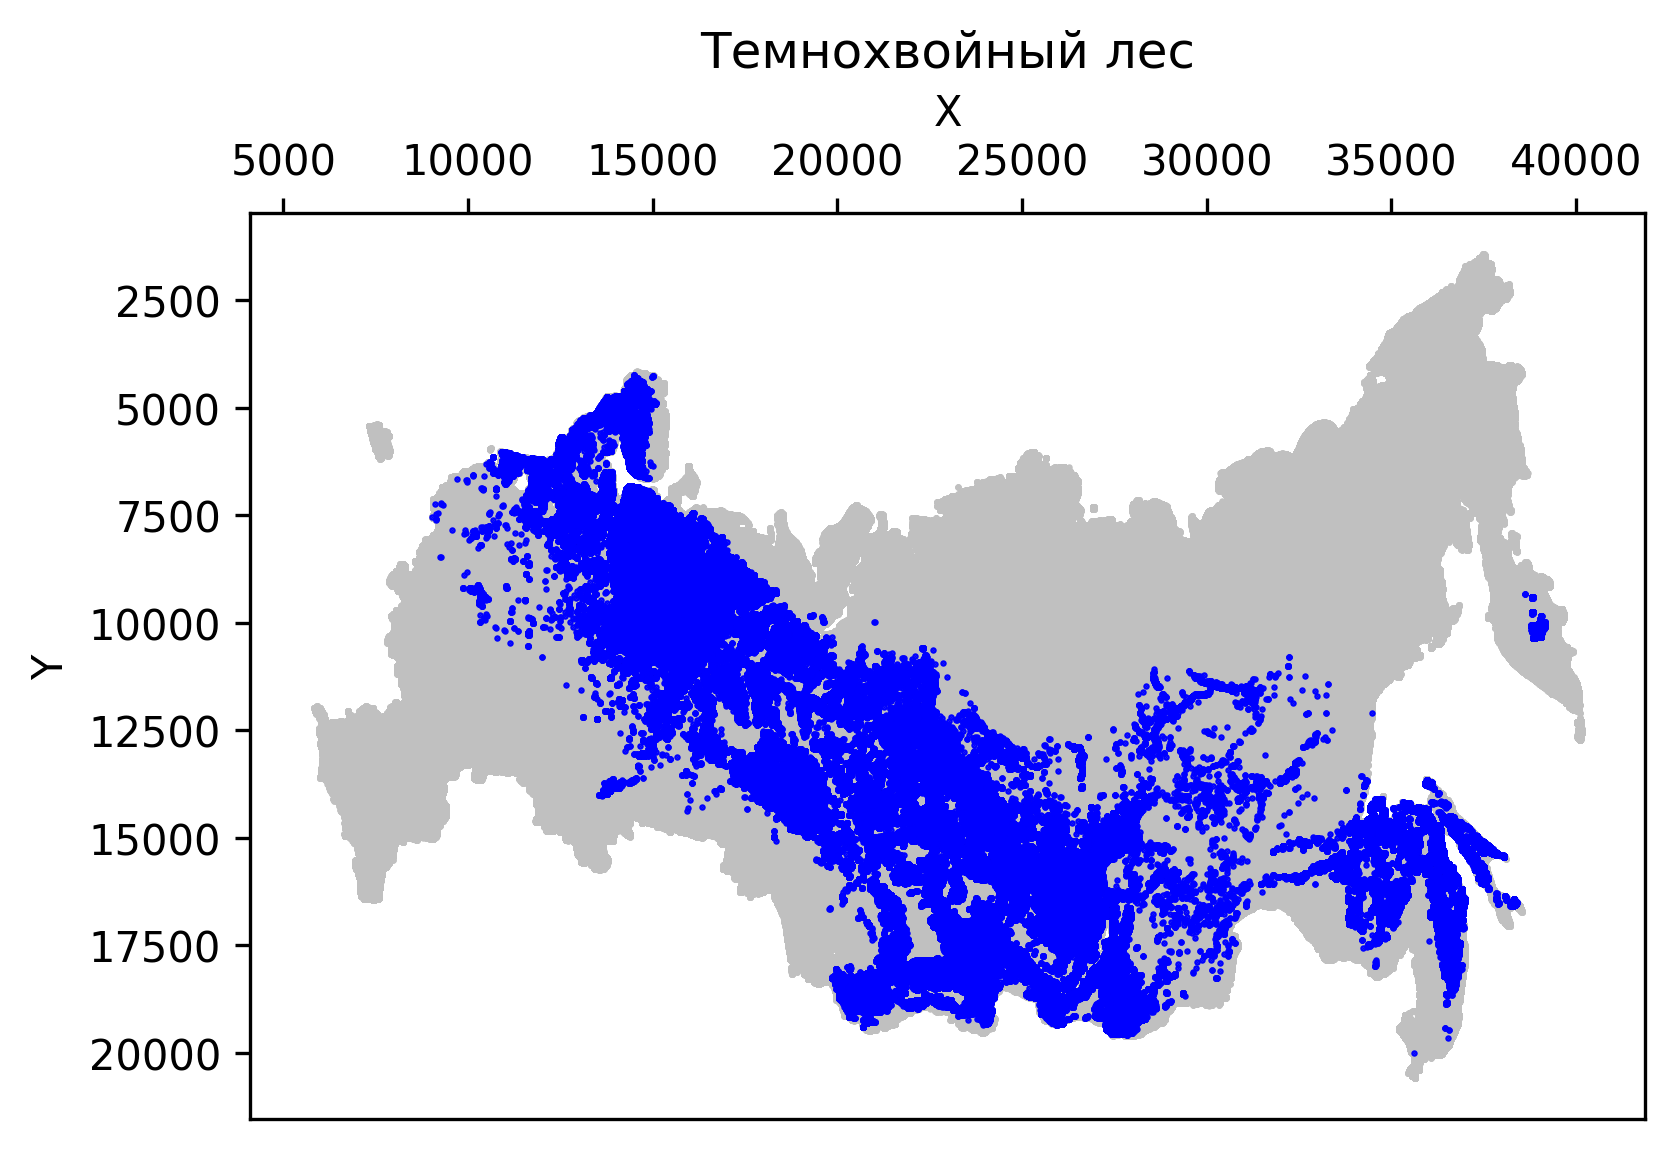
\includegraphics[]{class-1-map}
\end{figure}

\begin{figure}[H]
    \centering
    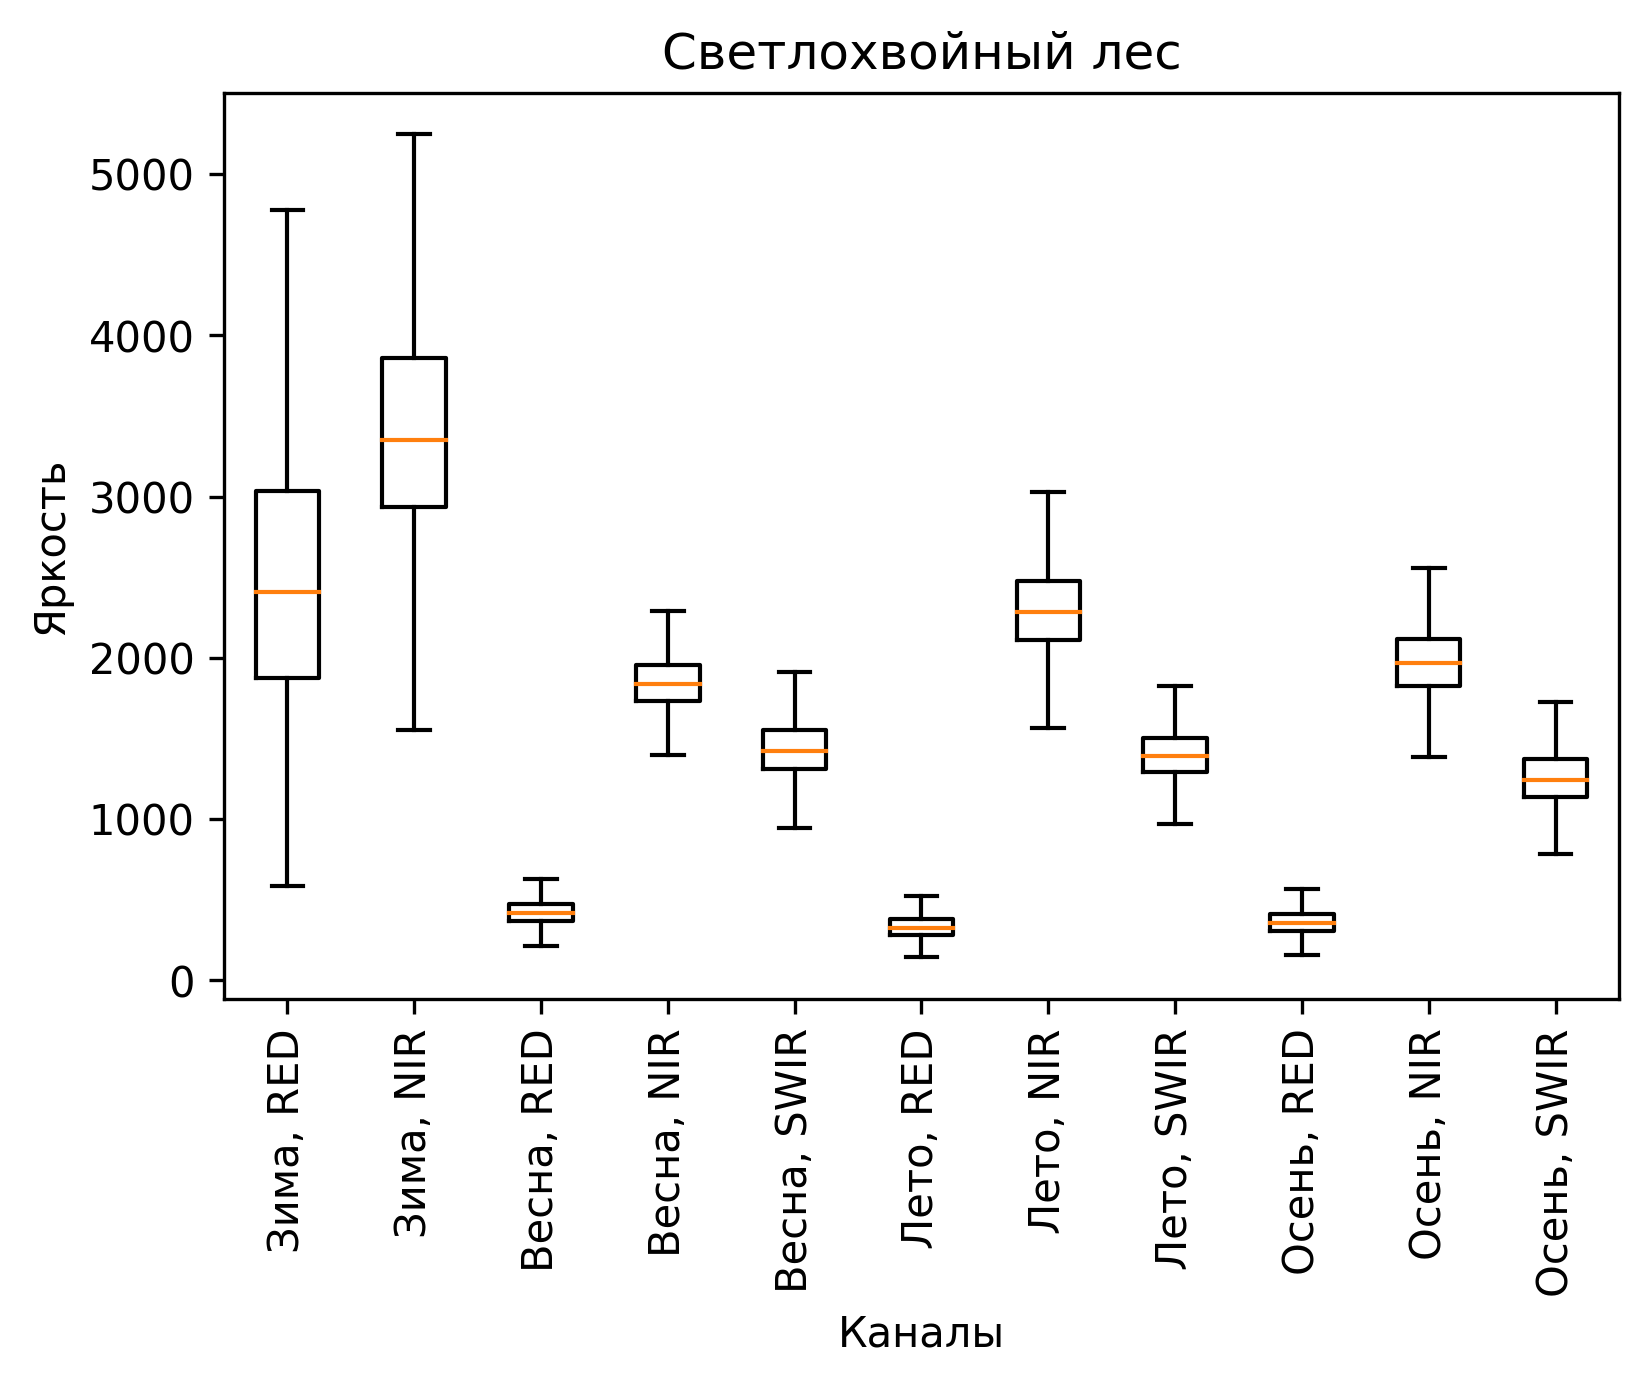
\includegraphics[]{class-2-boxplot}
    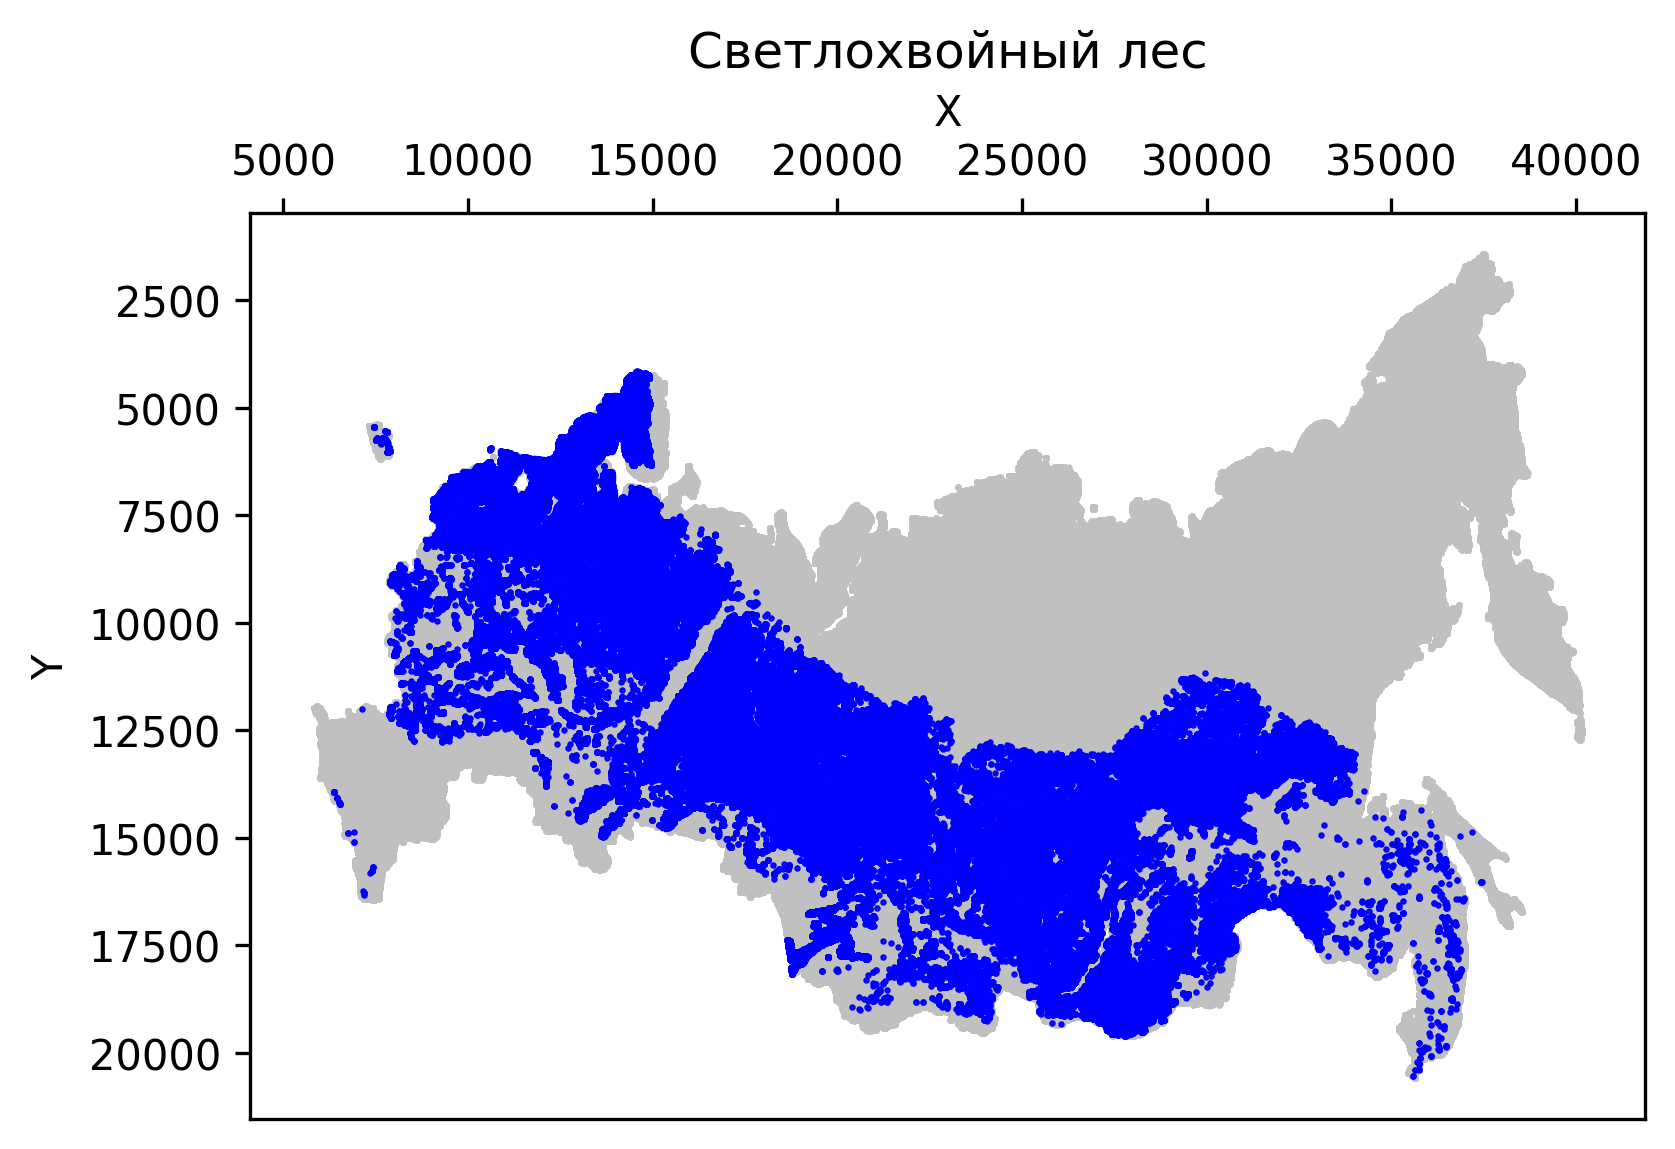
\includegraphics[]{class-2-map}
\end{figure}

\begin{figure}[H]
    \centering
    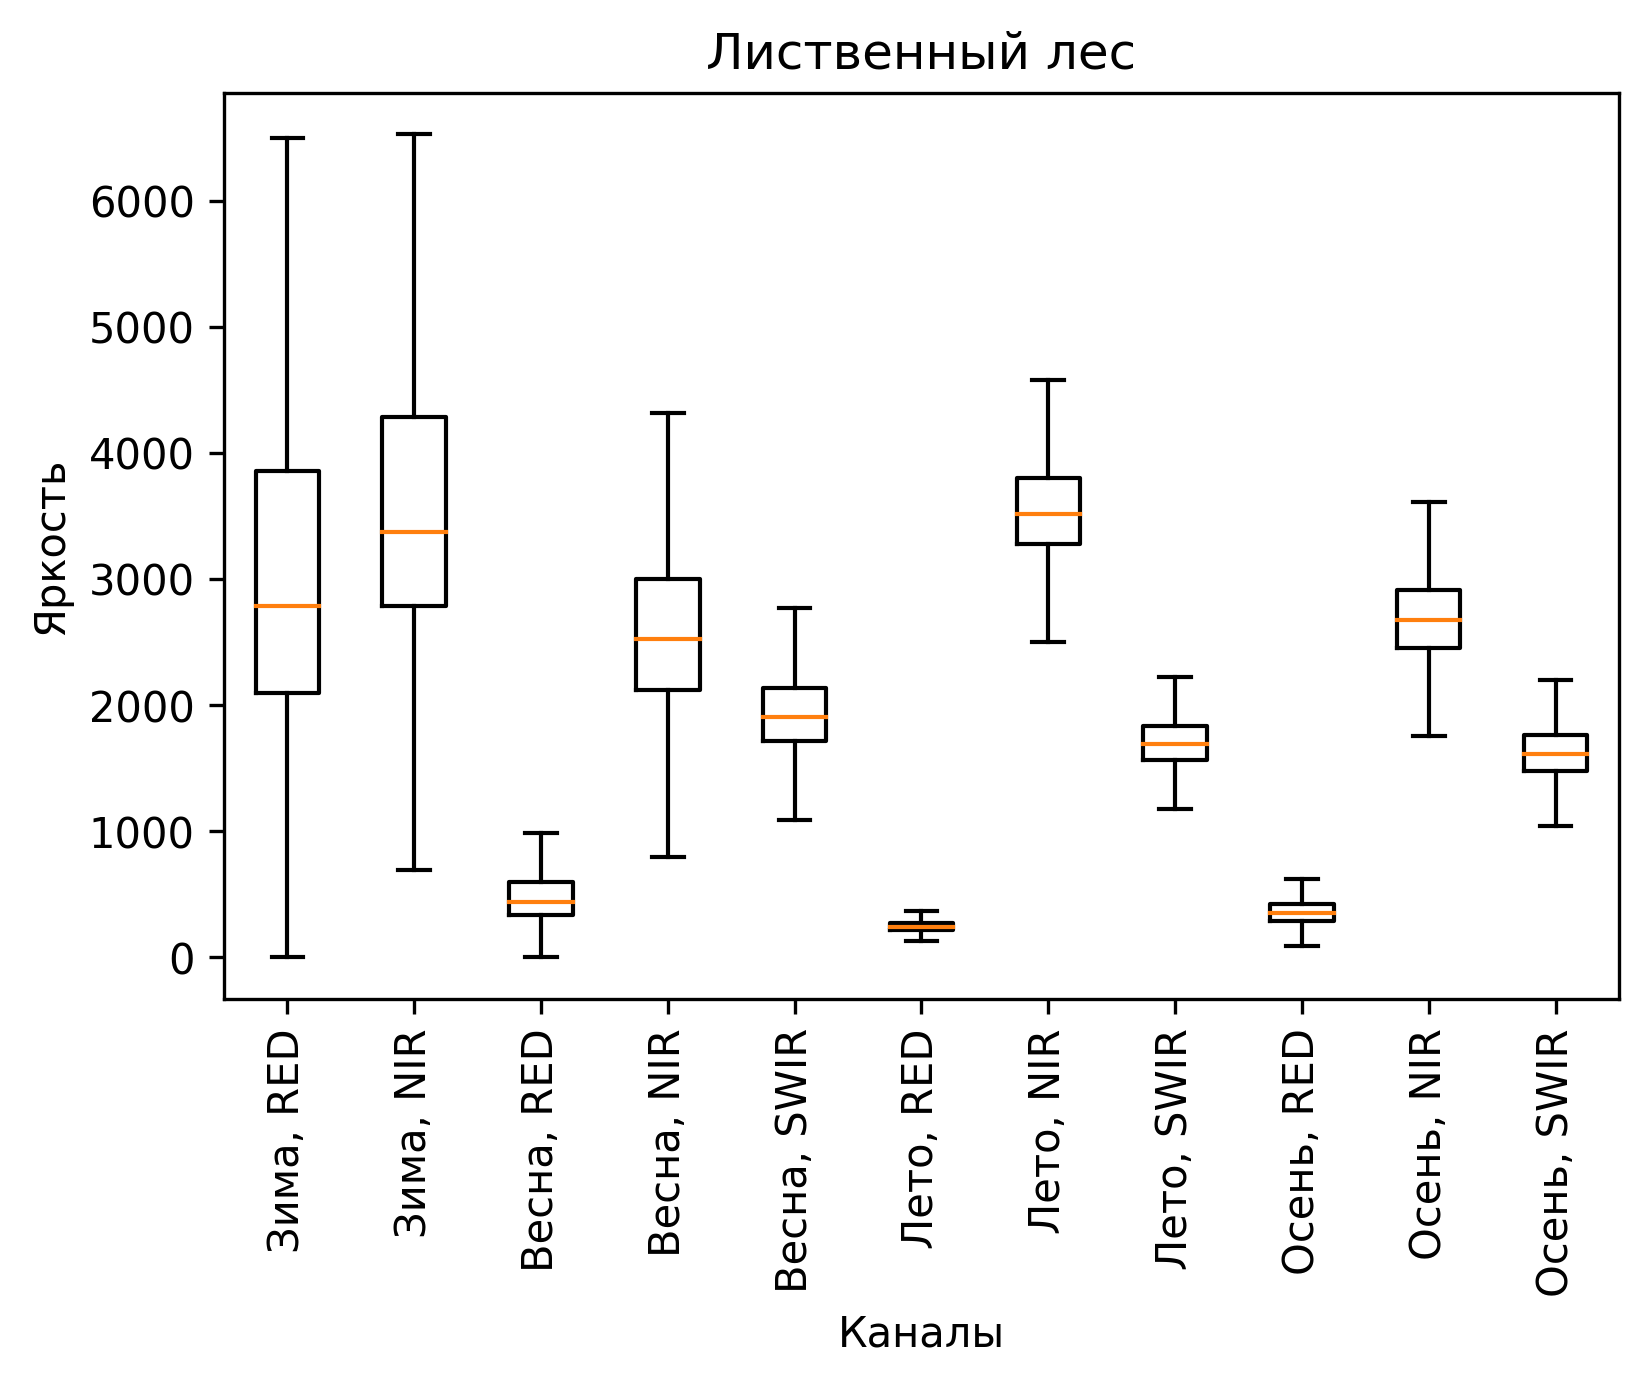
\includegraphics[]{class-3-boxplot}
    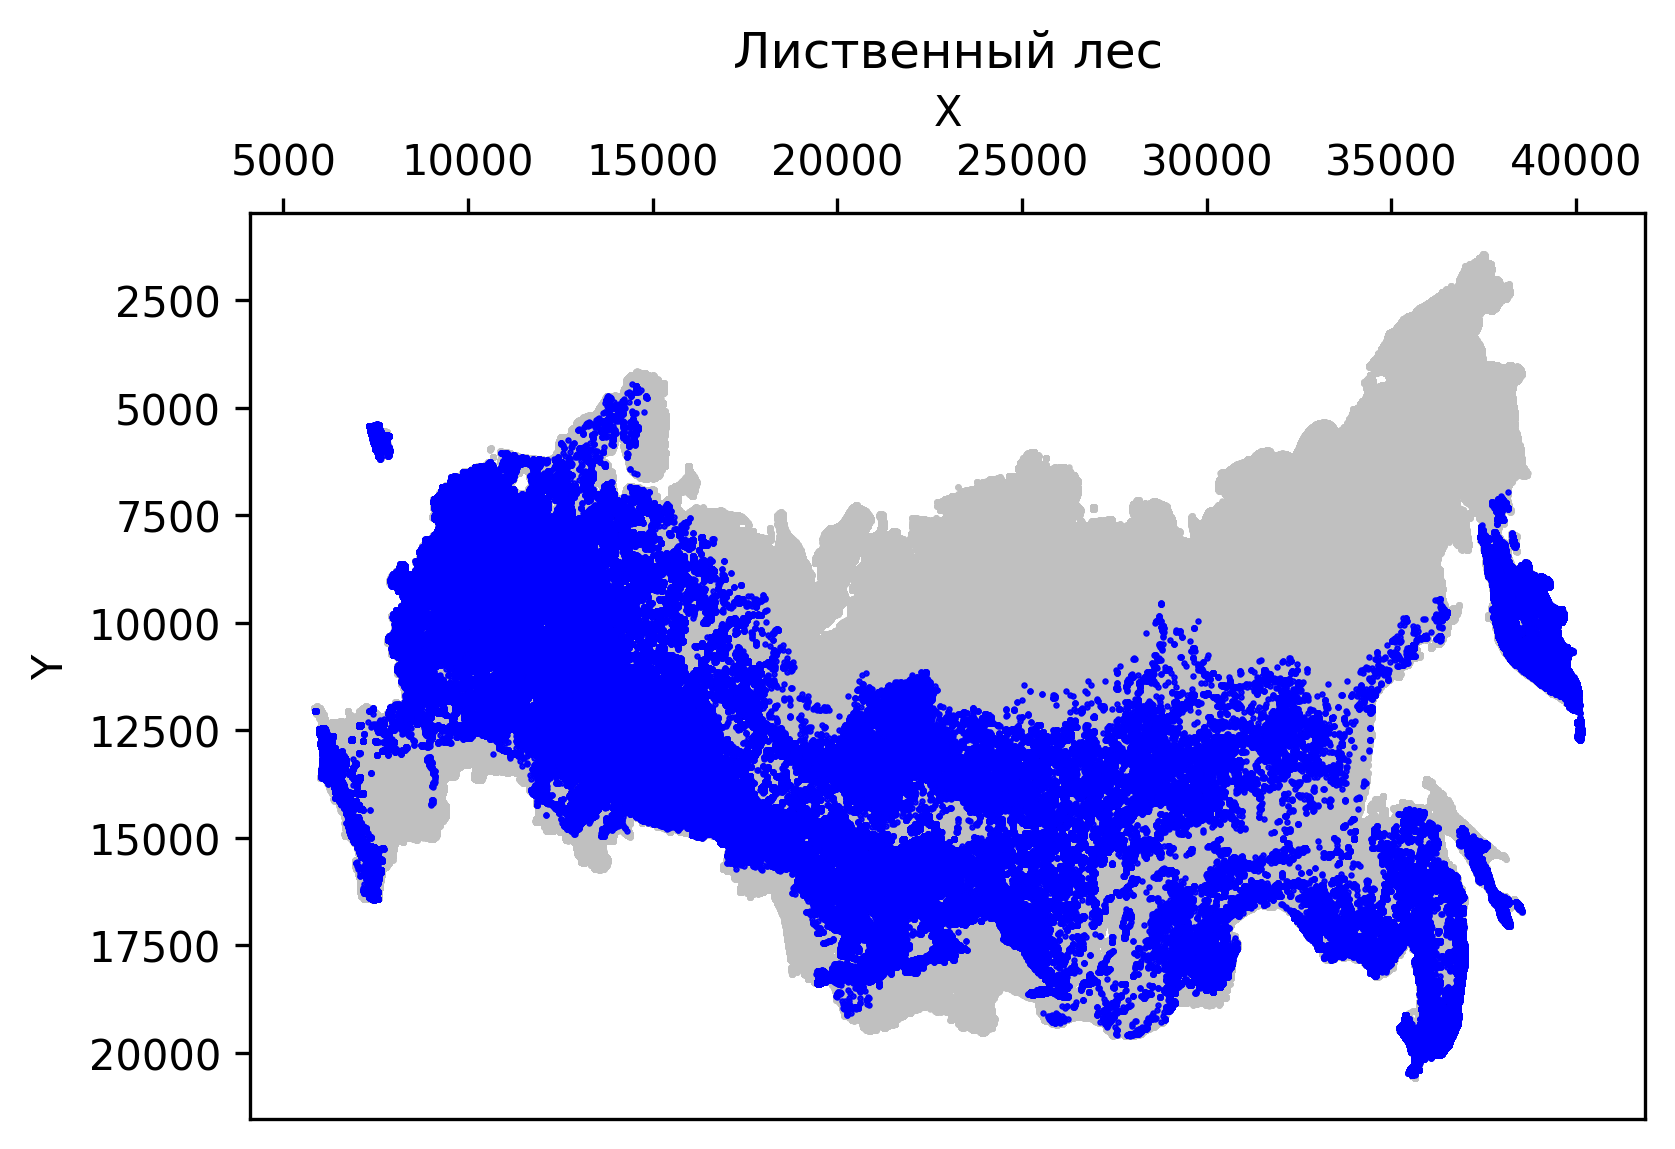
\includegraphics[]{class-3-map}
\end{figure}

\begin{figure}[H]
    \centering
    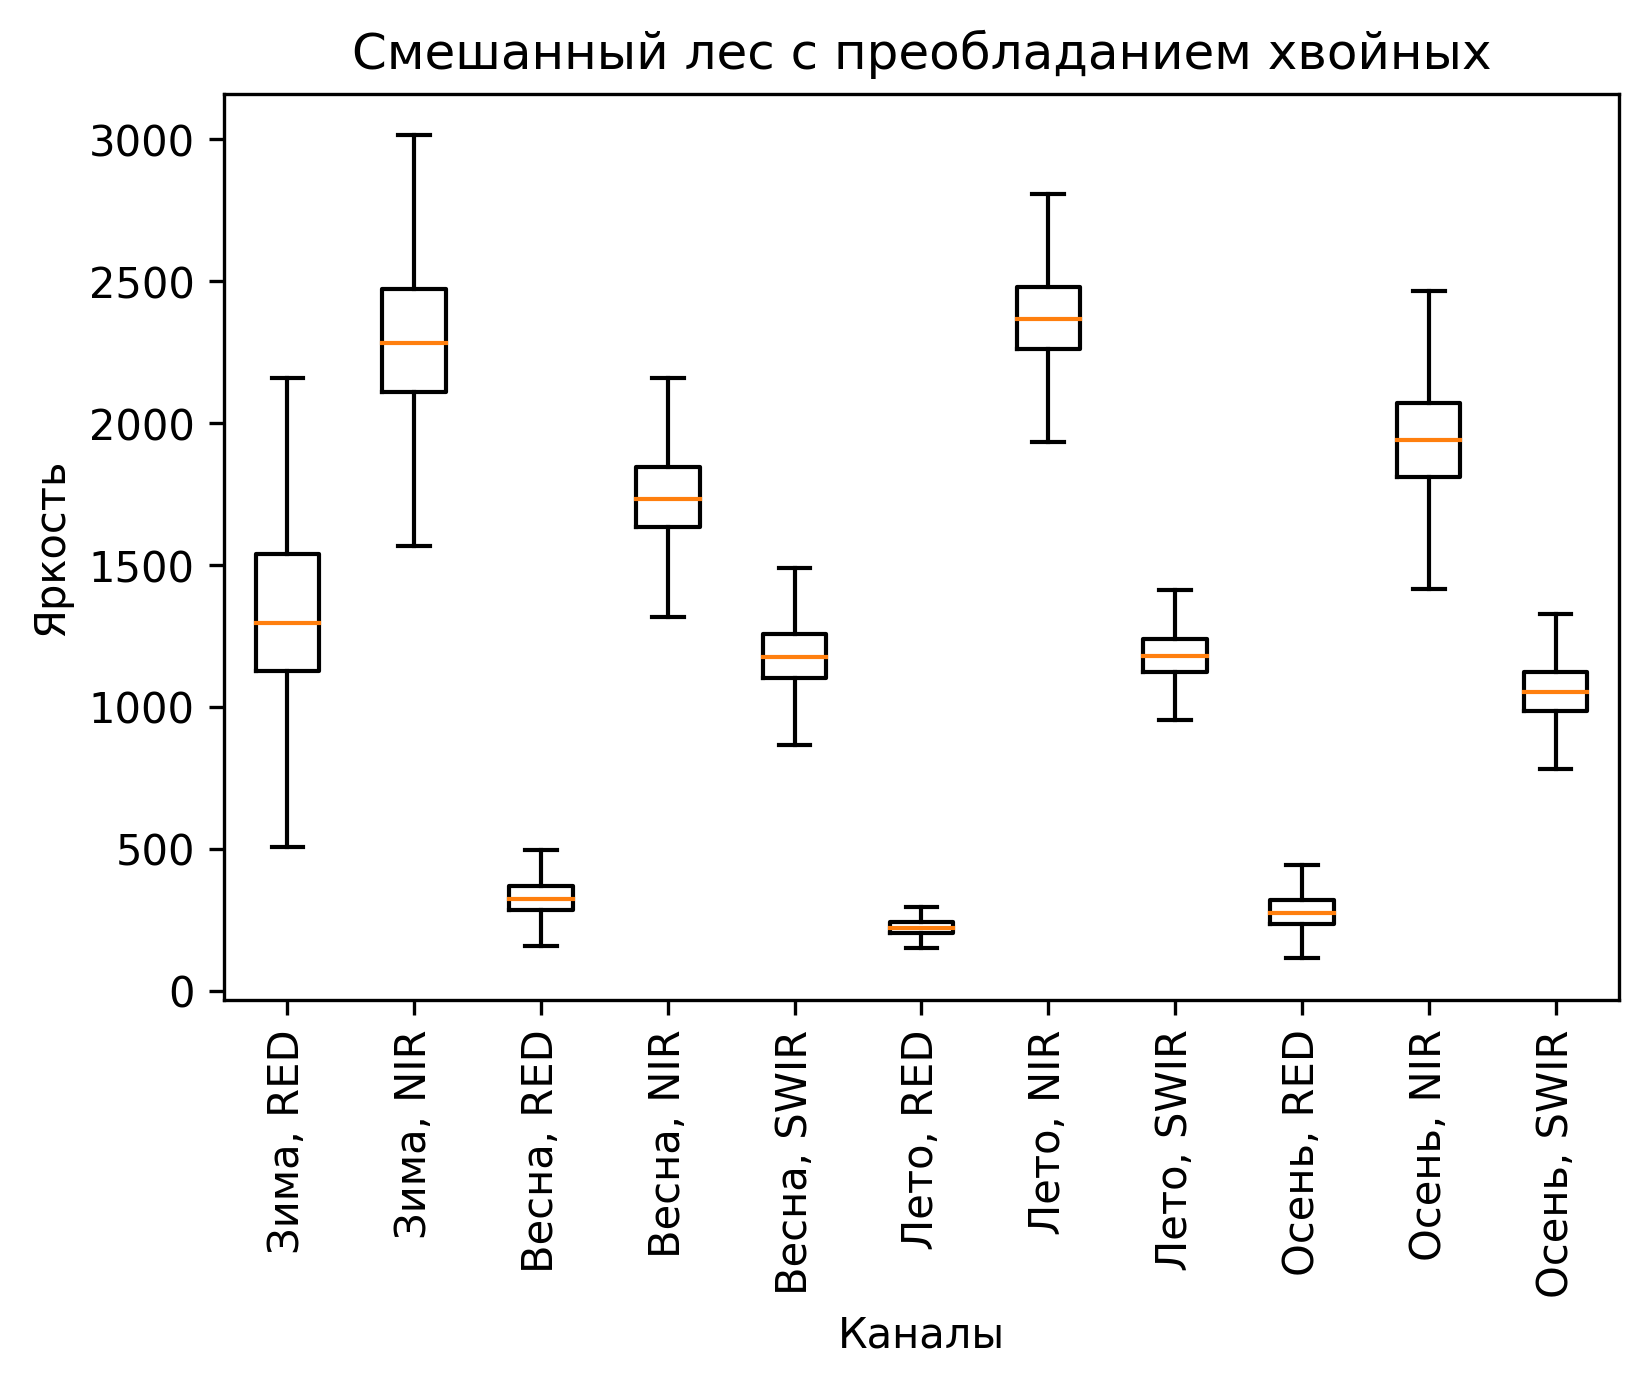
\includegraphics[]{class-10-boxplot}
    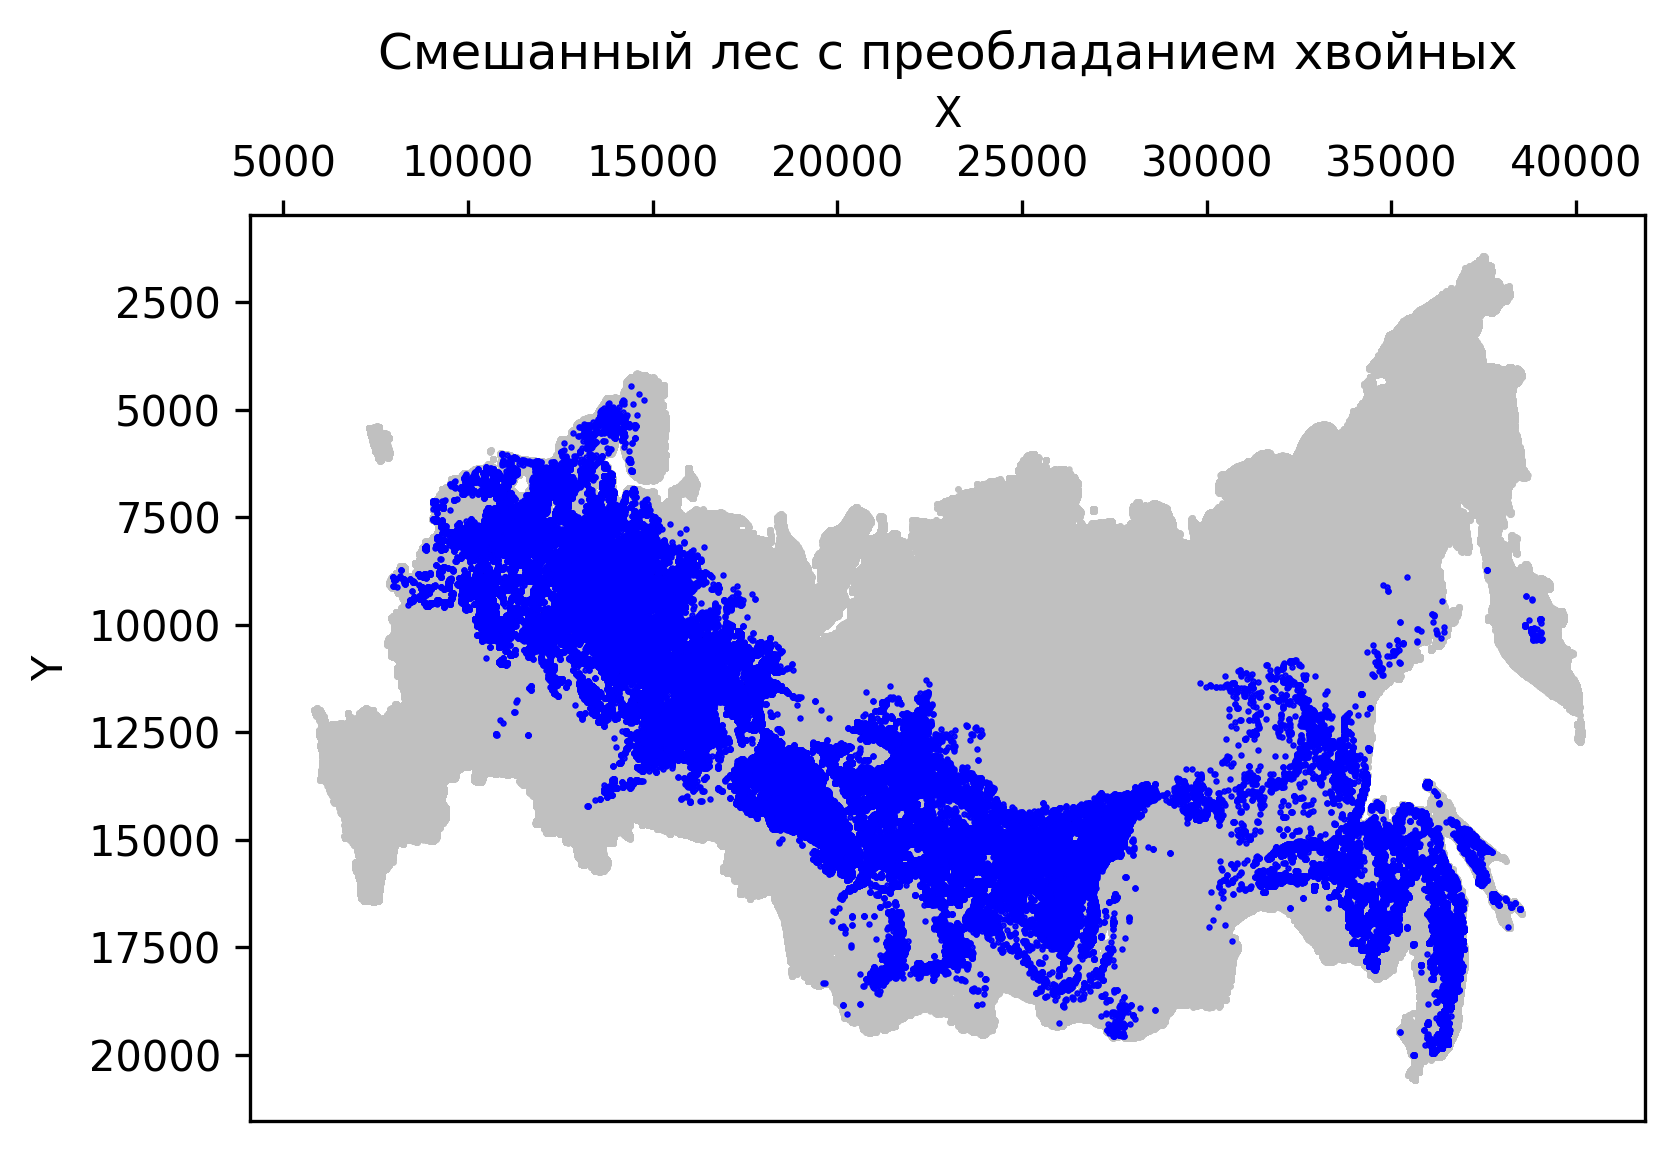
\includegraphics[]{class-10-map}
\end{figure}

\begin{figure}[H]
    \centering
    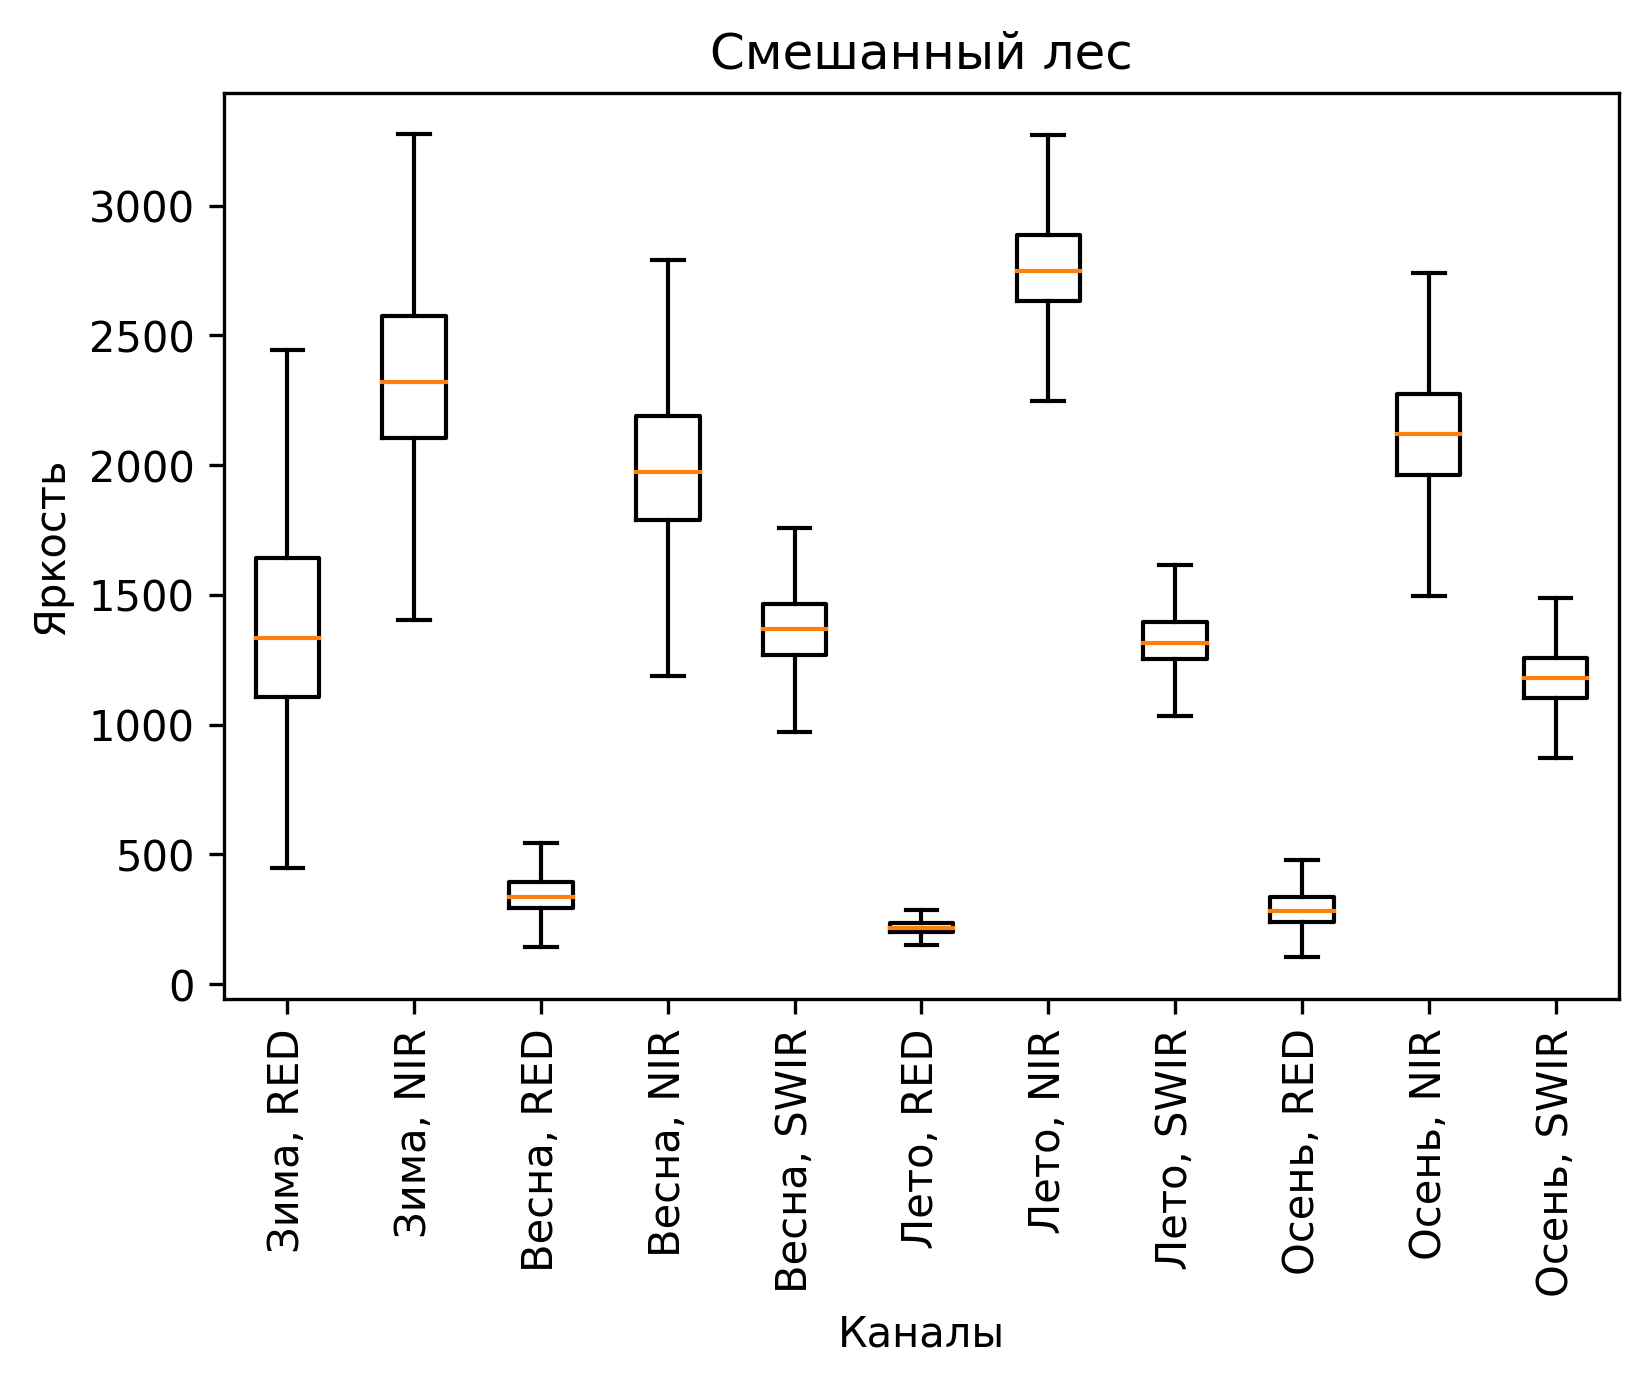
\includegraphics[]{class-11-boxplot}
    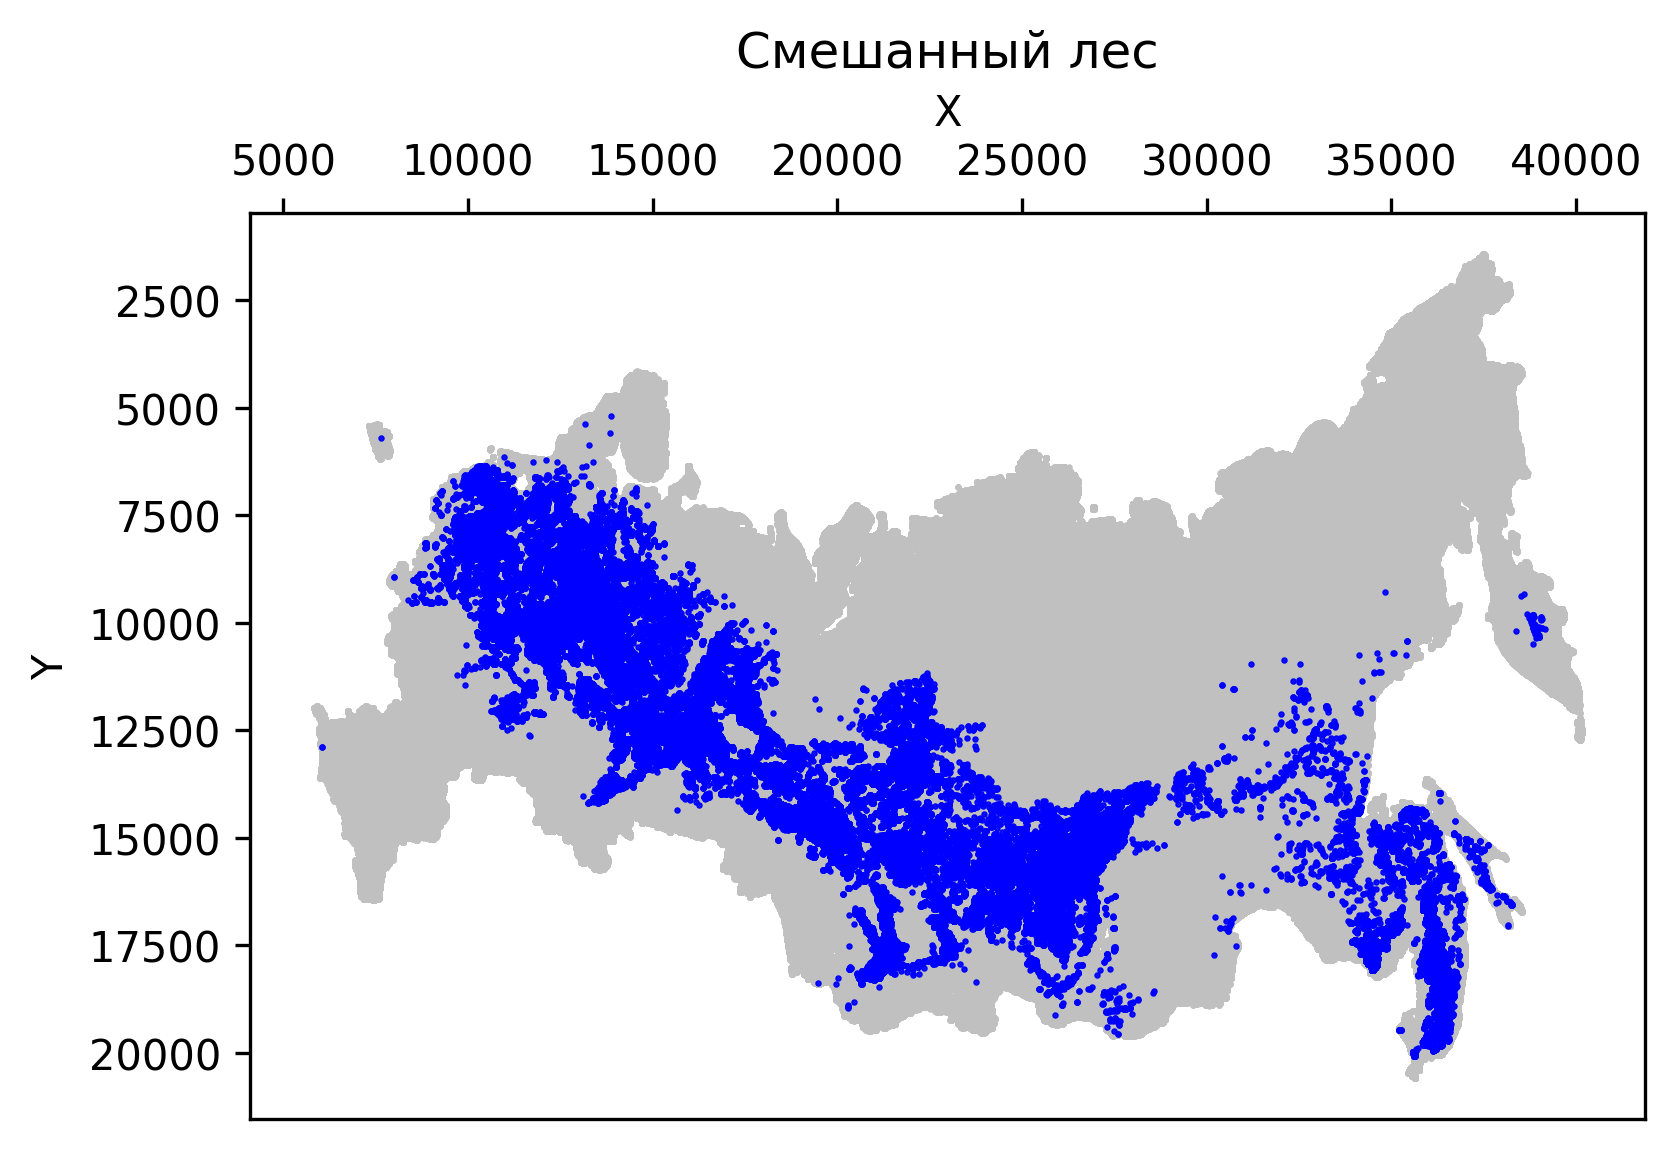
\includegraphics[]{class-11-map}
\end{figure}

\begin{figure}[H]
    \centering
    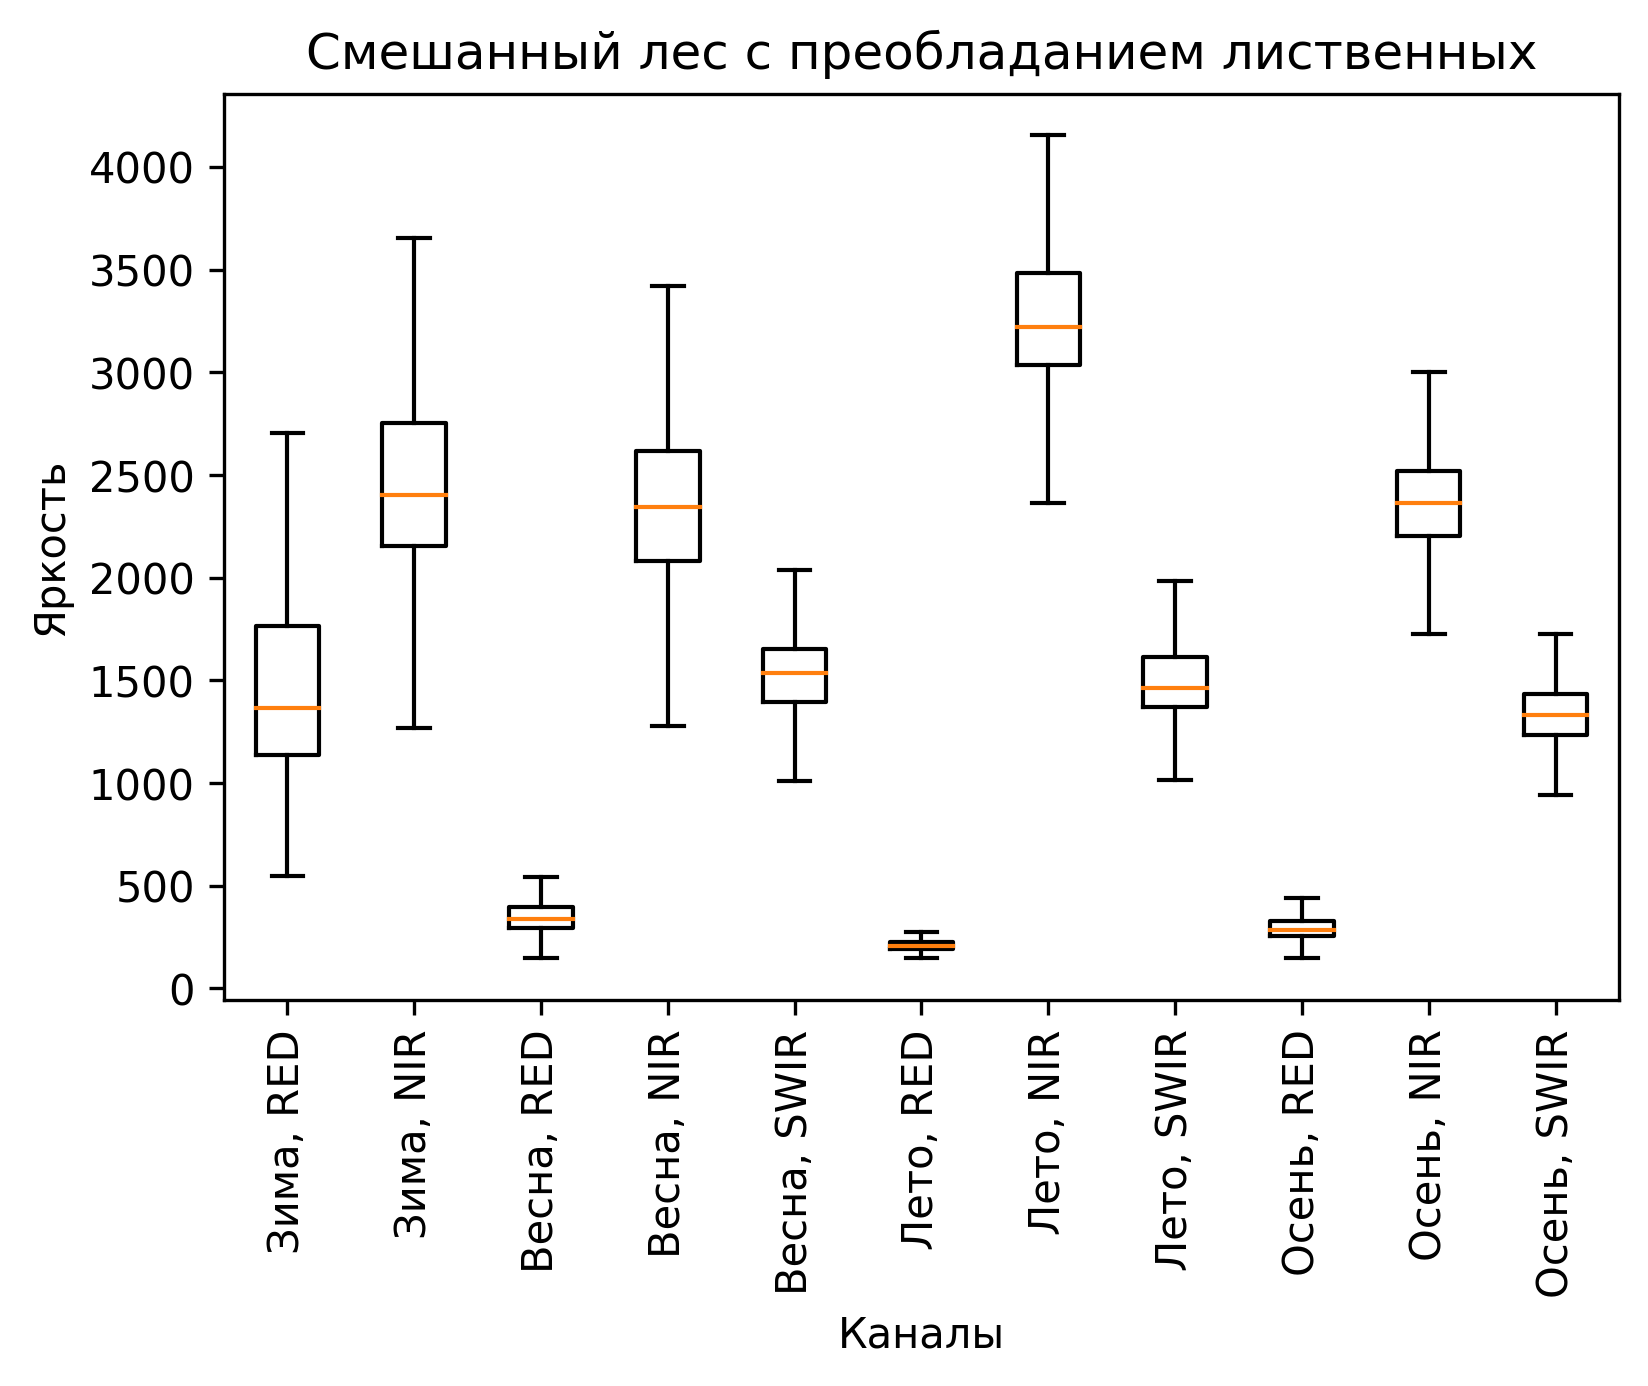
\includegraphics[]{class-12-boxplot}
    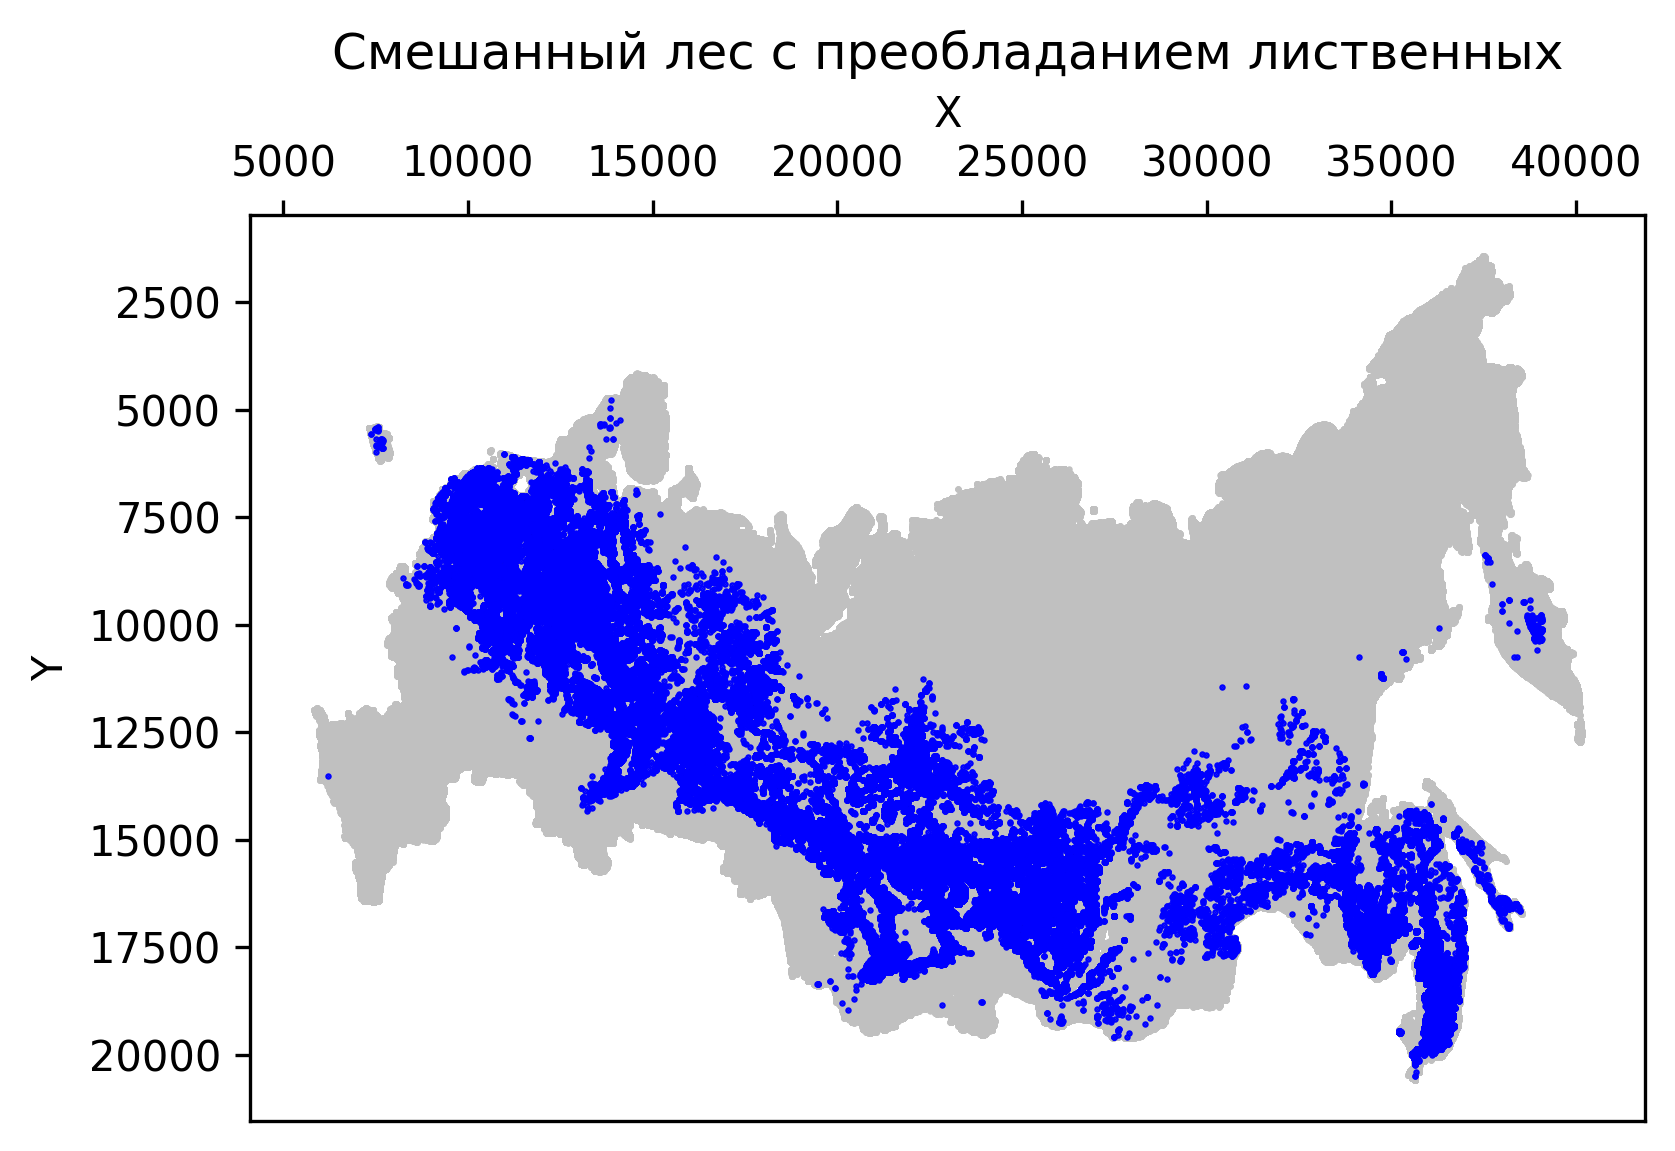
\includegraphics[]{class-12-map}
\end{figure}

\begin{figure}[H]
    \centering
    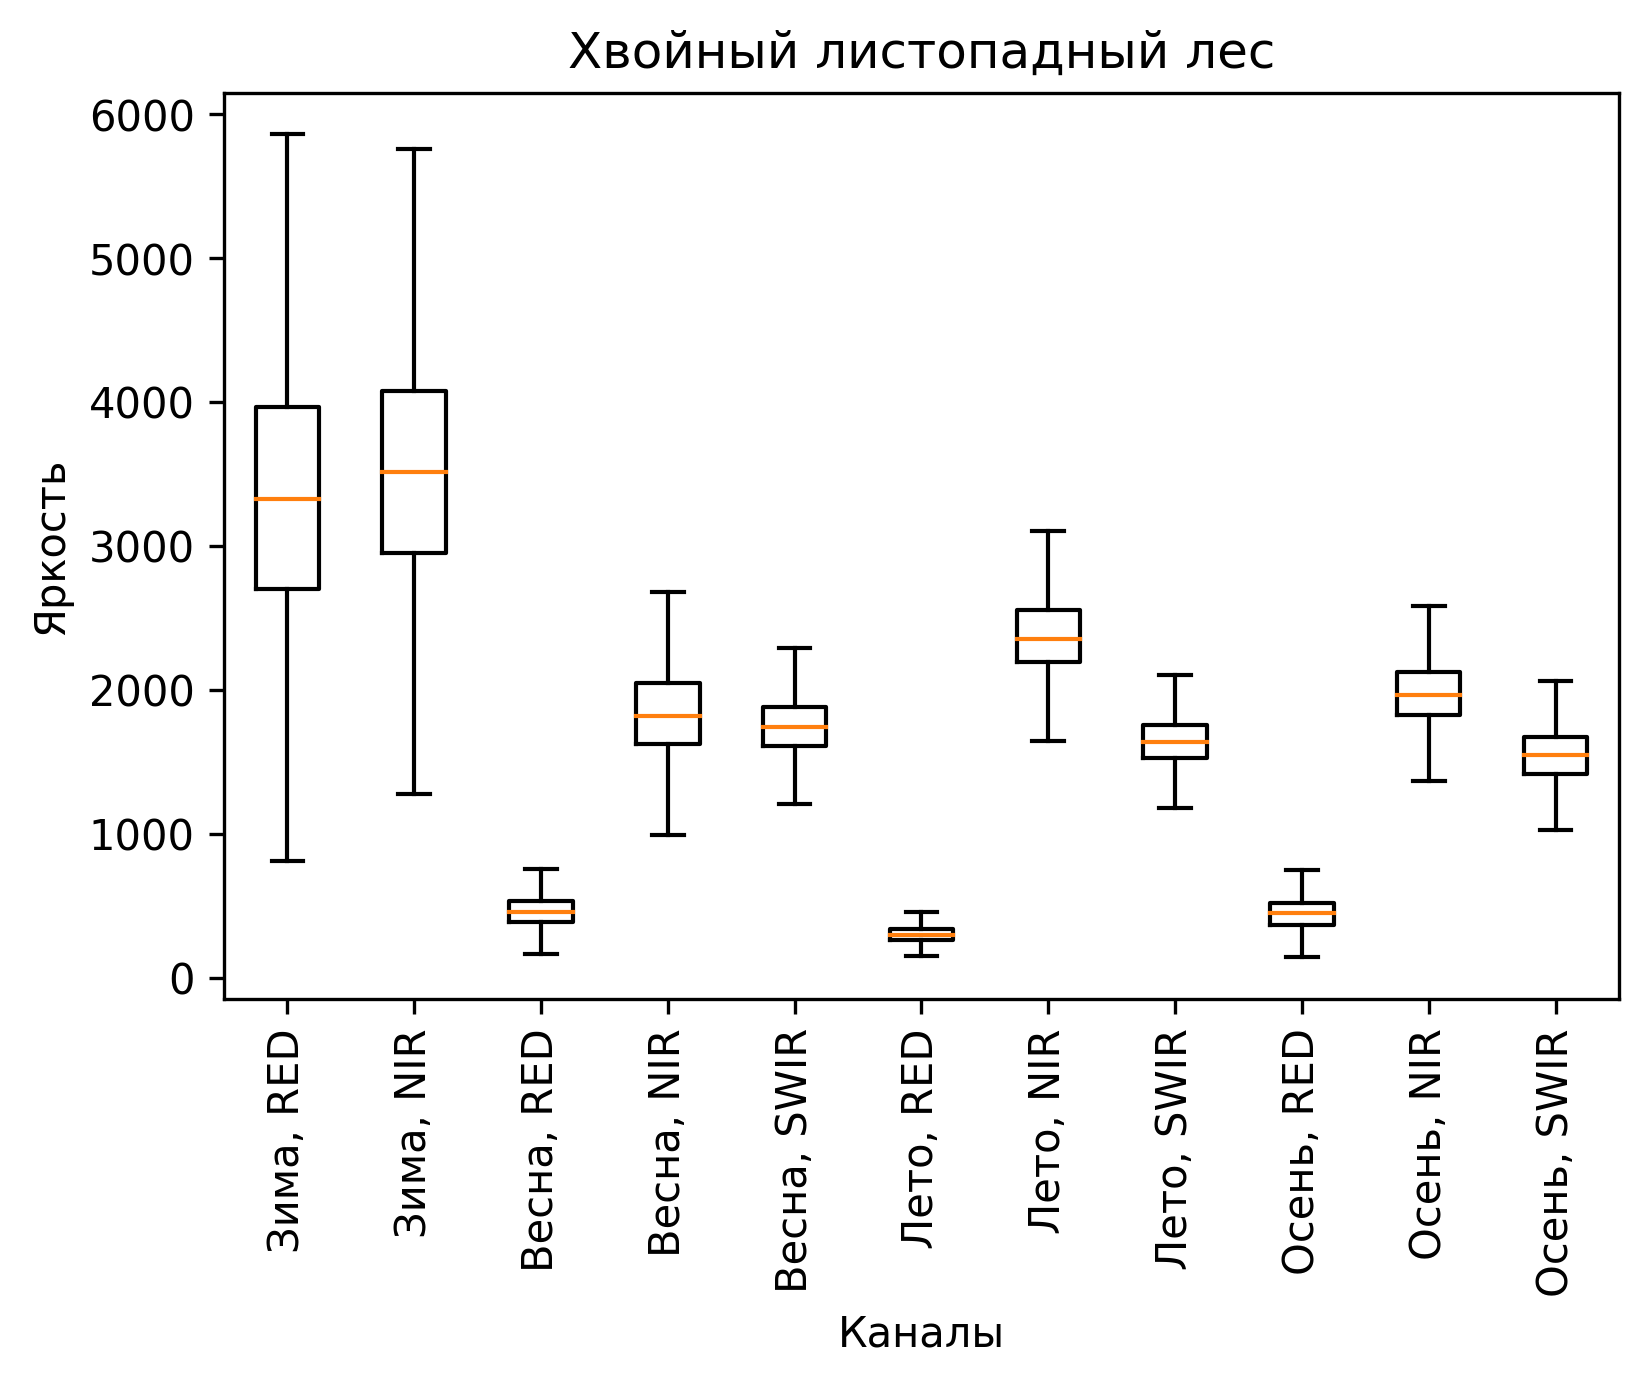
\includegraphics[]{class-4-boxplot}
    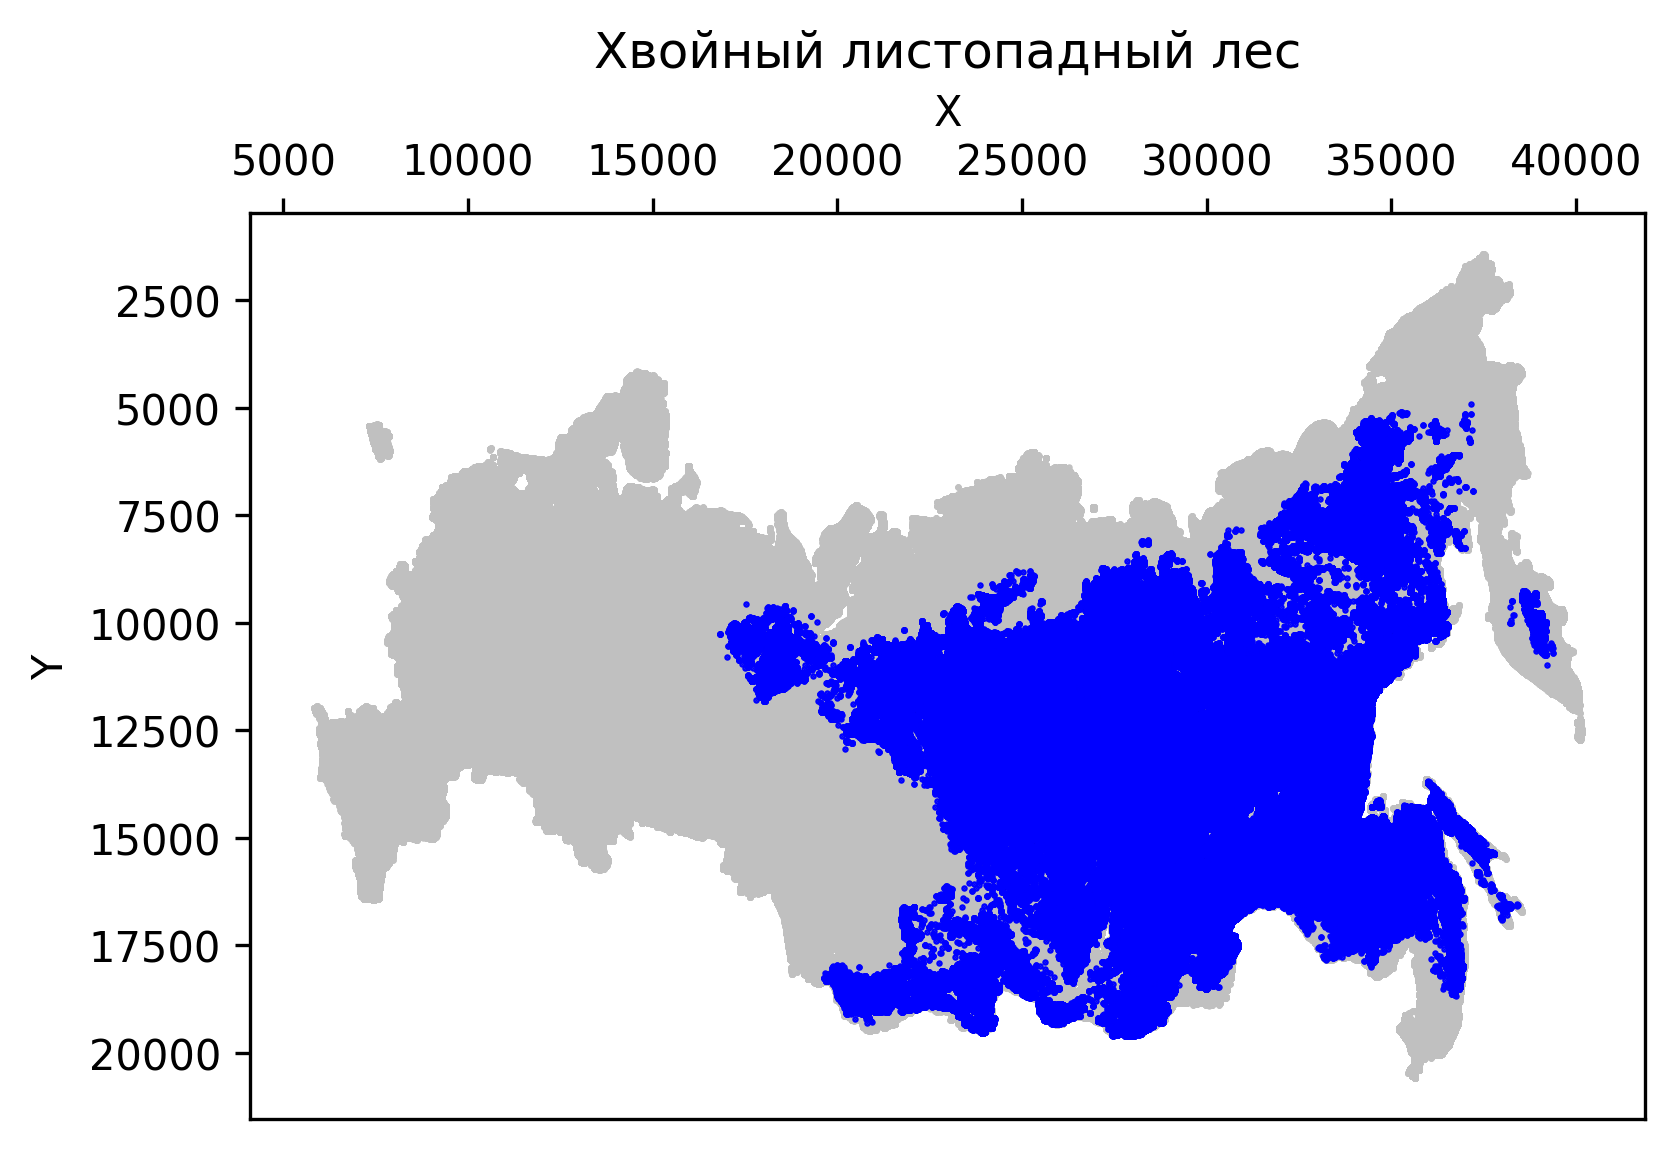
\includegraphics[]{class-4-map}
\end{figure}

\begin{figure}[H]
    \centering
    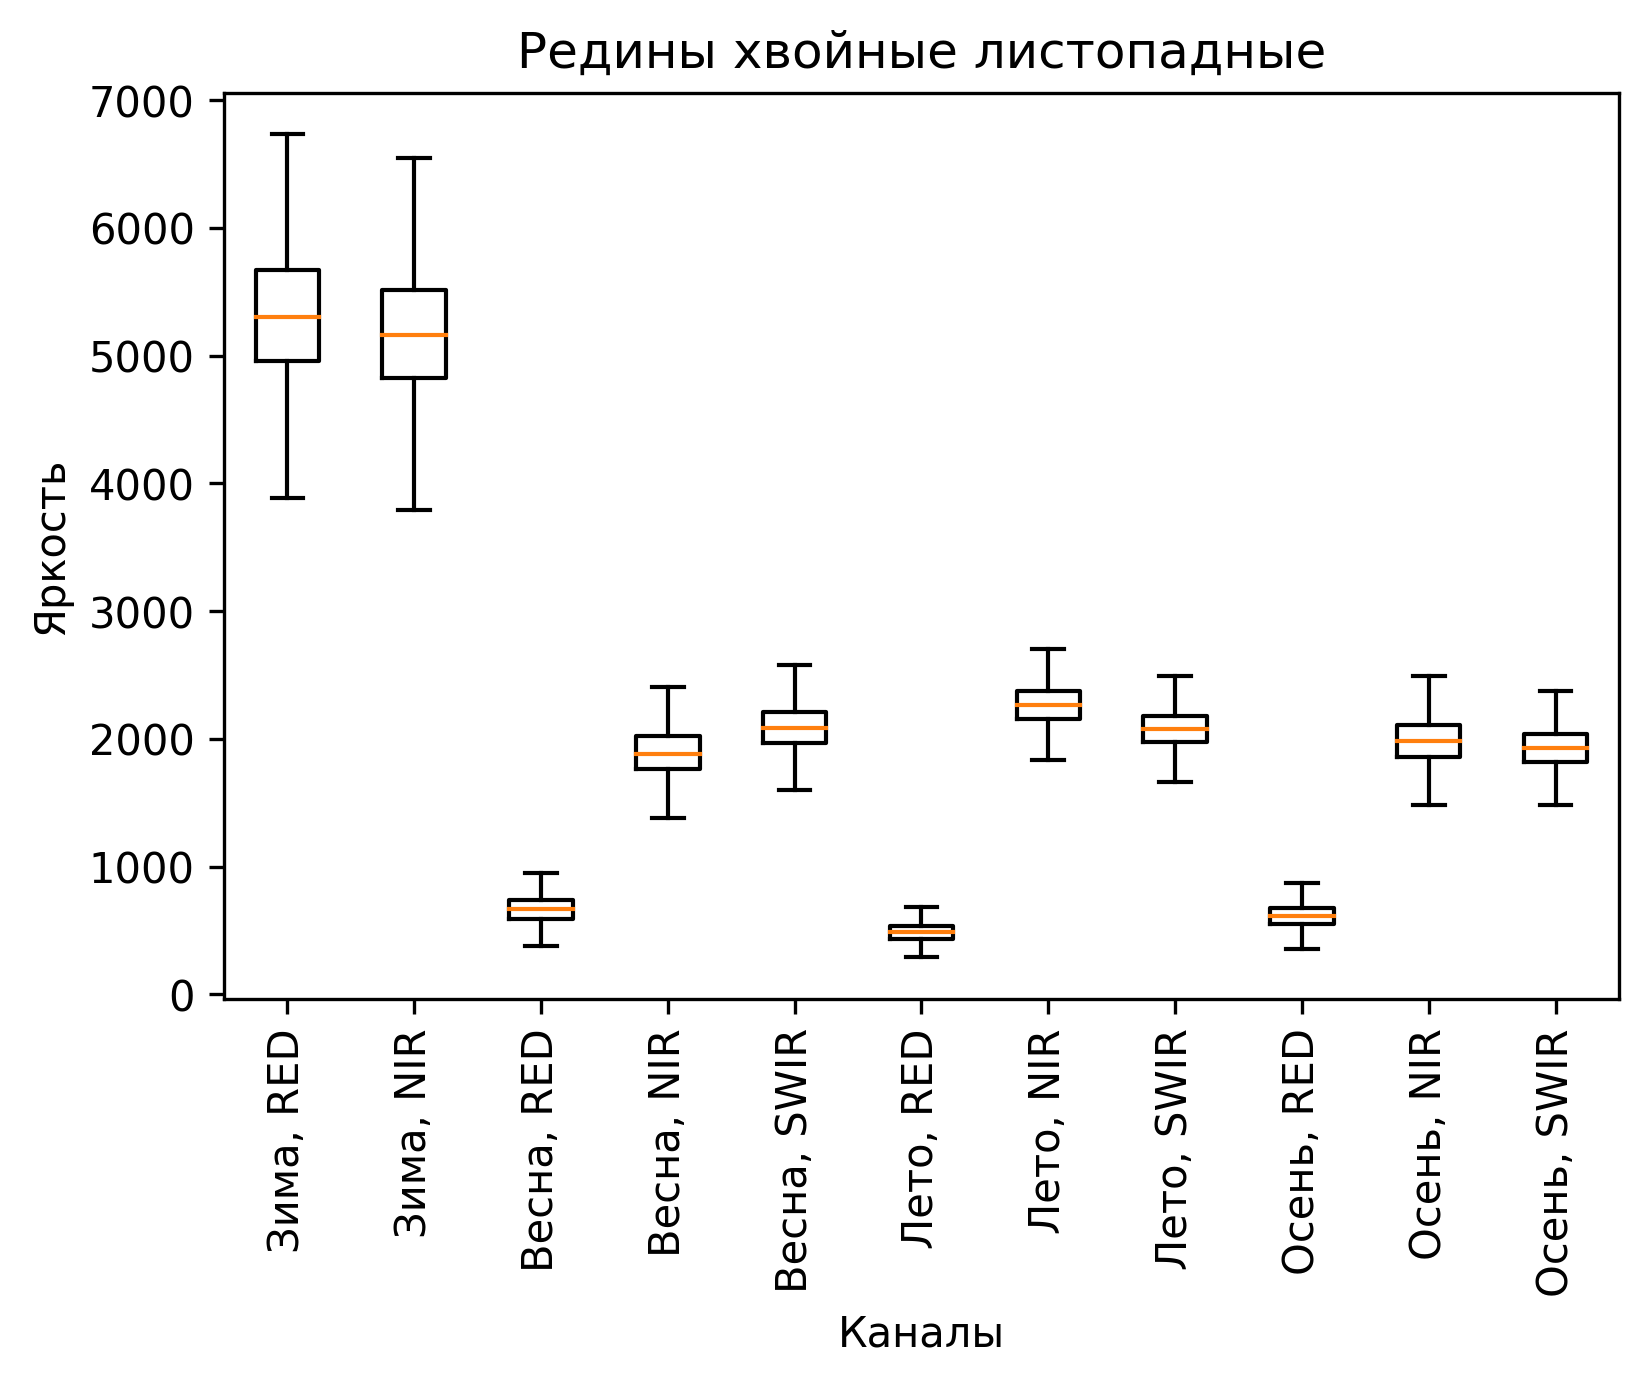
\includegraphics[]{class-23-boxplot}
    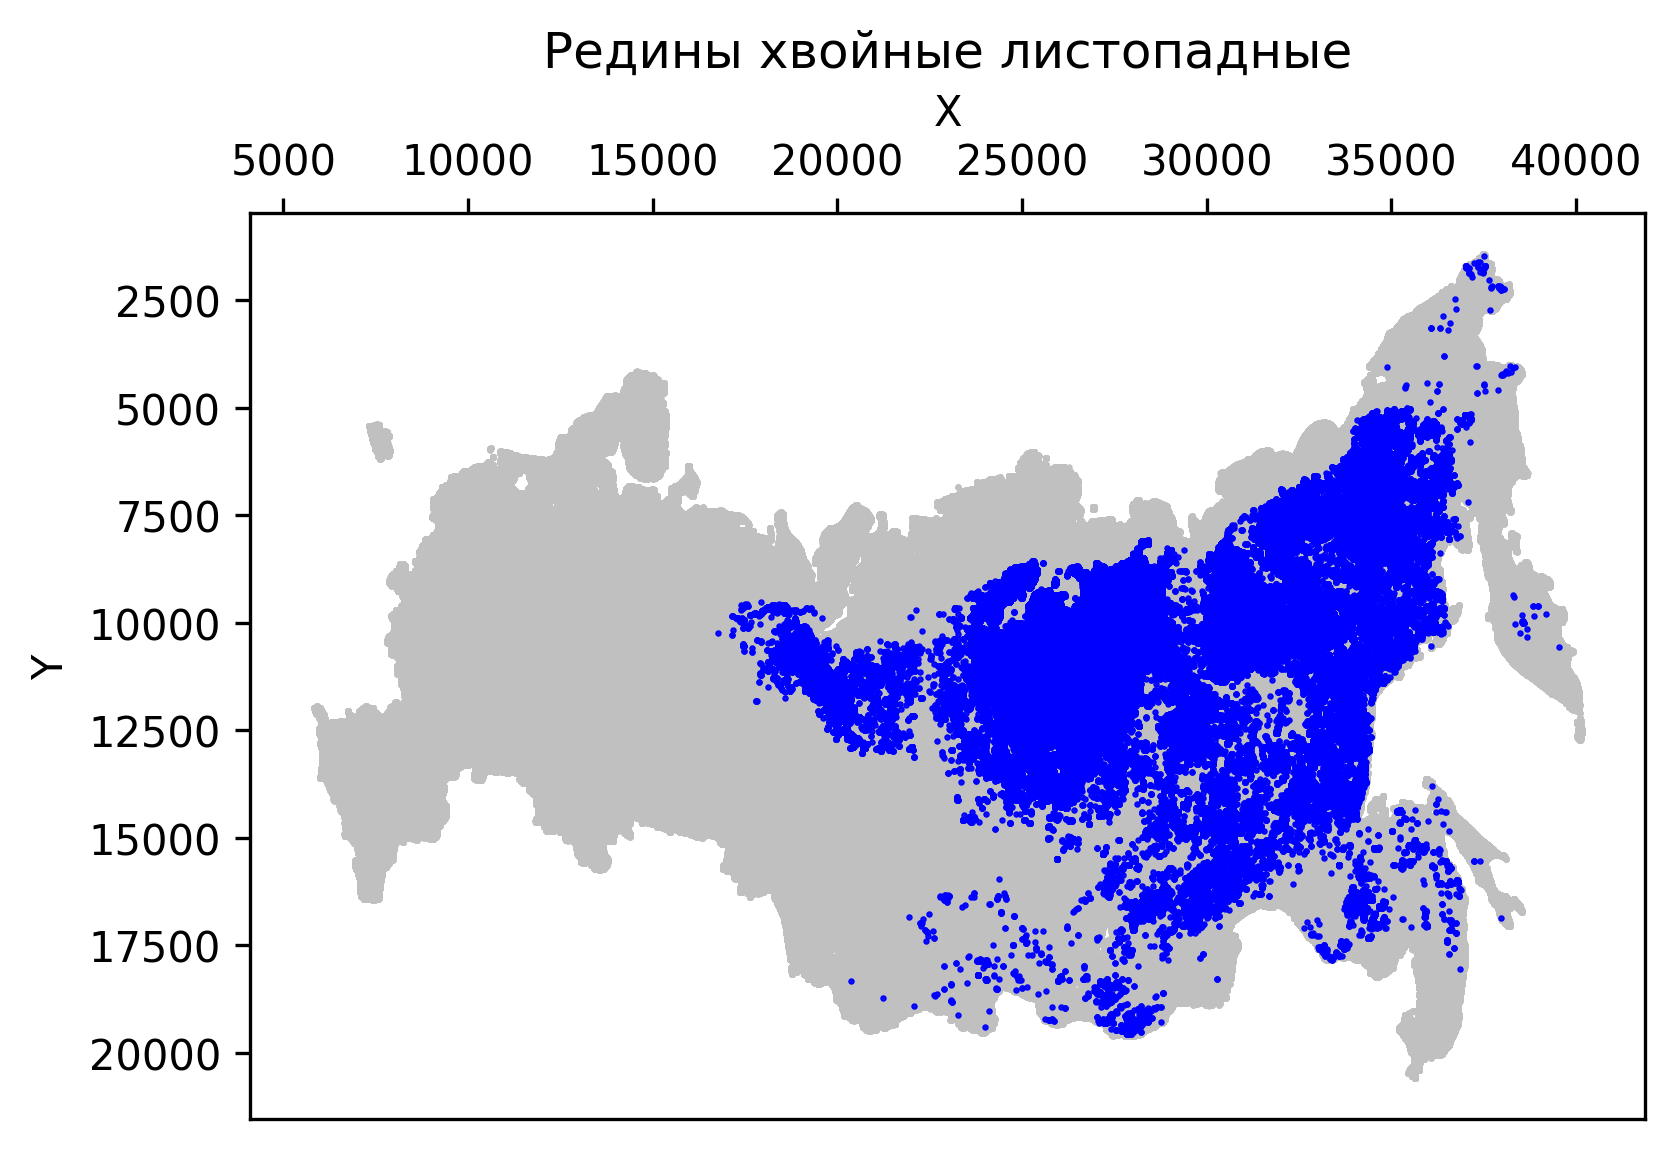
\includegraphics[]{class-23-map}
\end{figure}

\begin{figure}[H]
    \centering
    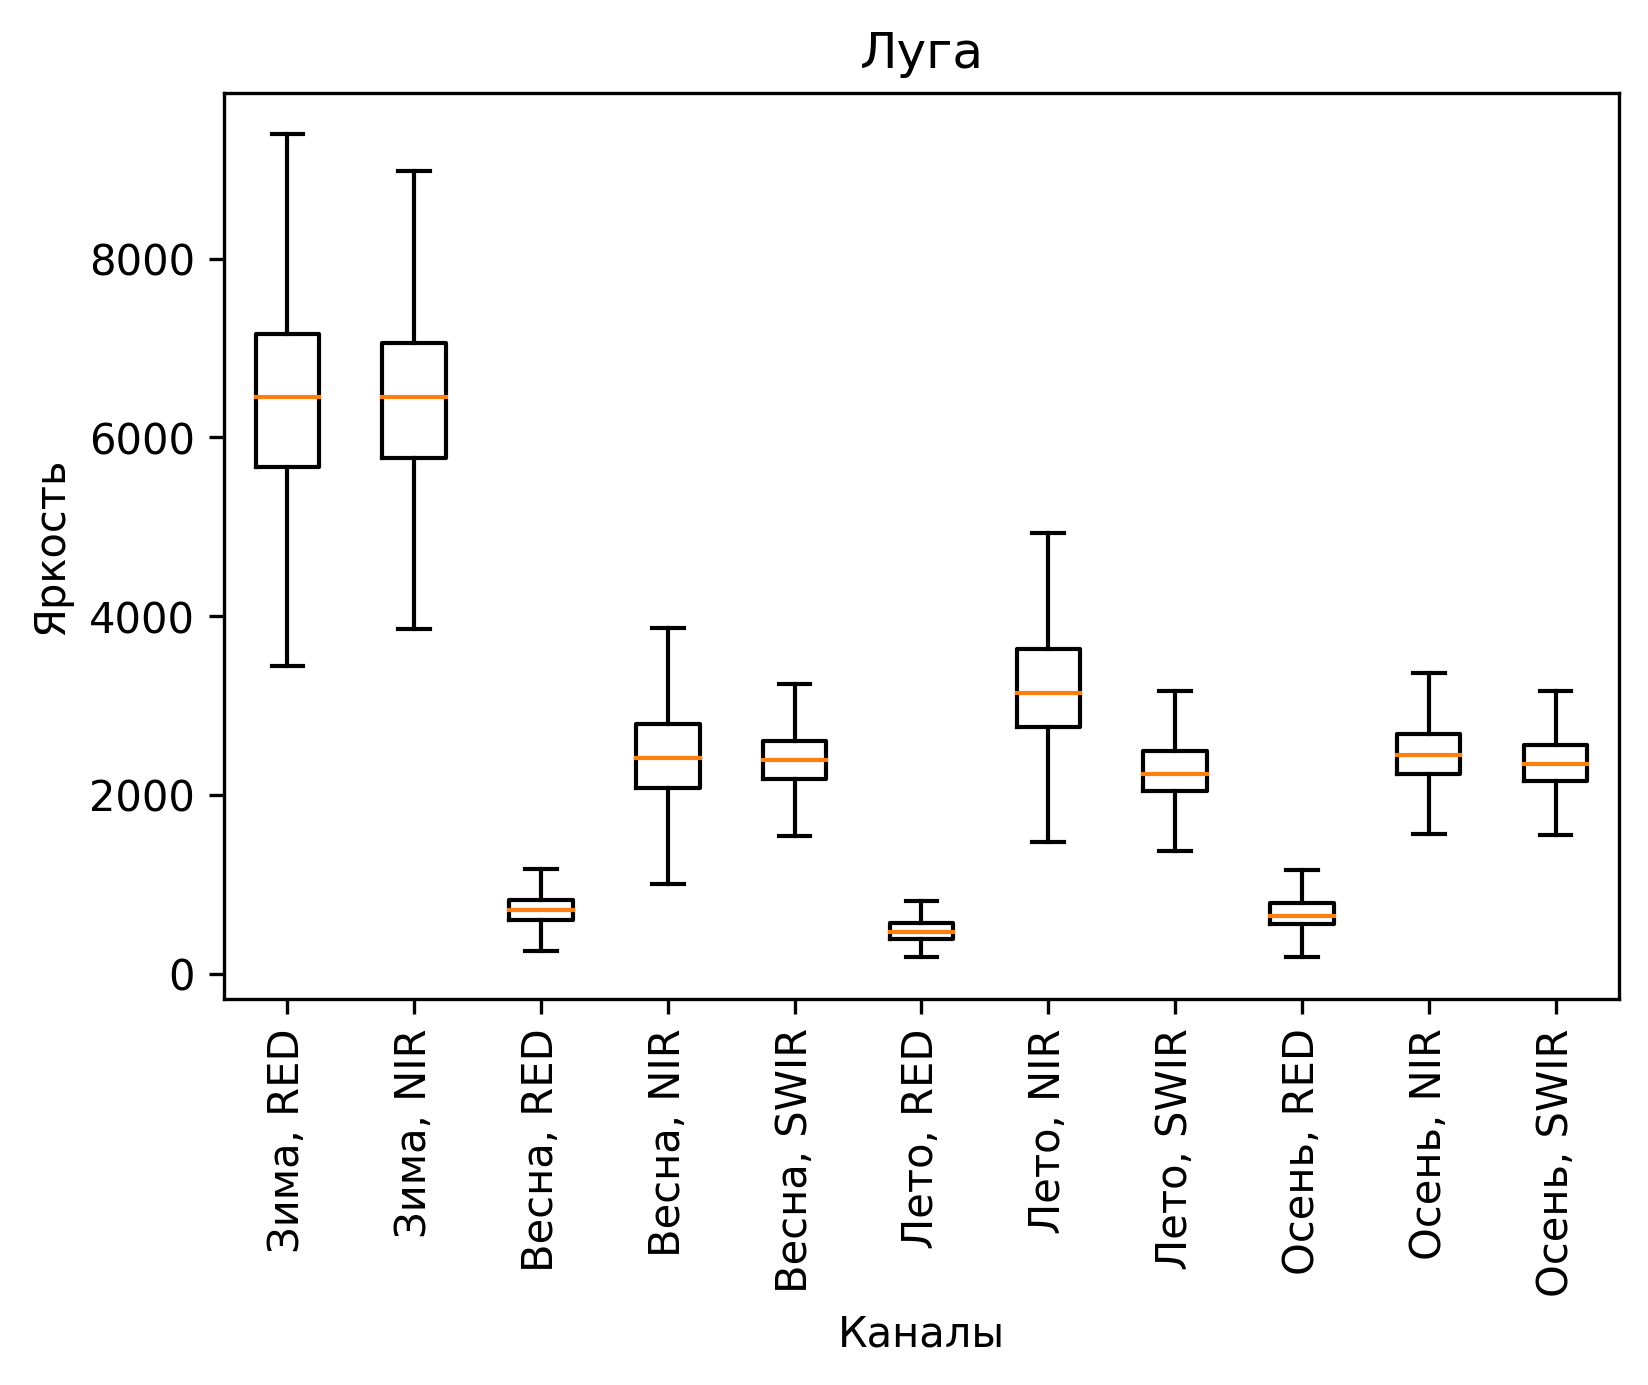
\includegraphics[]{class-8-boxplot}
    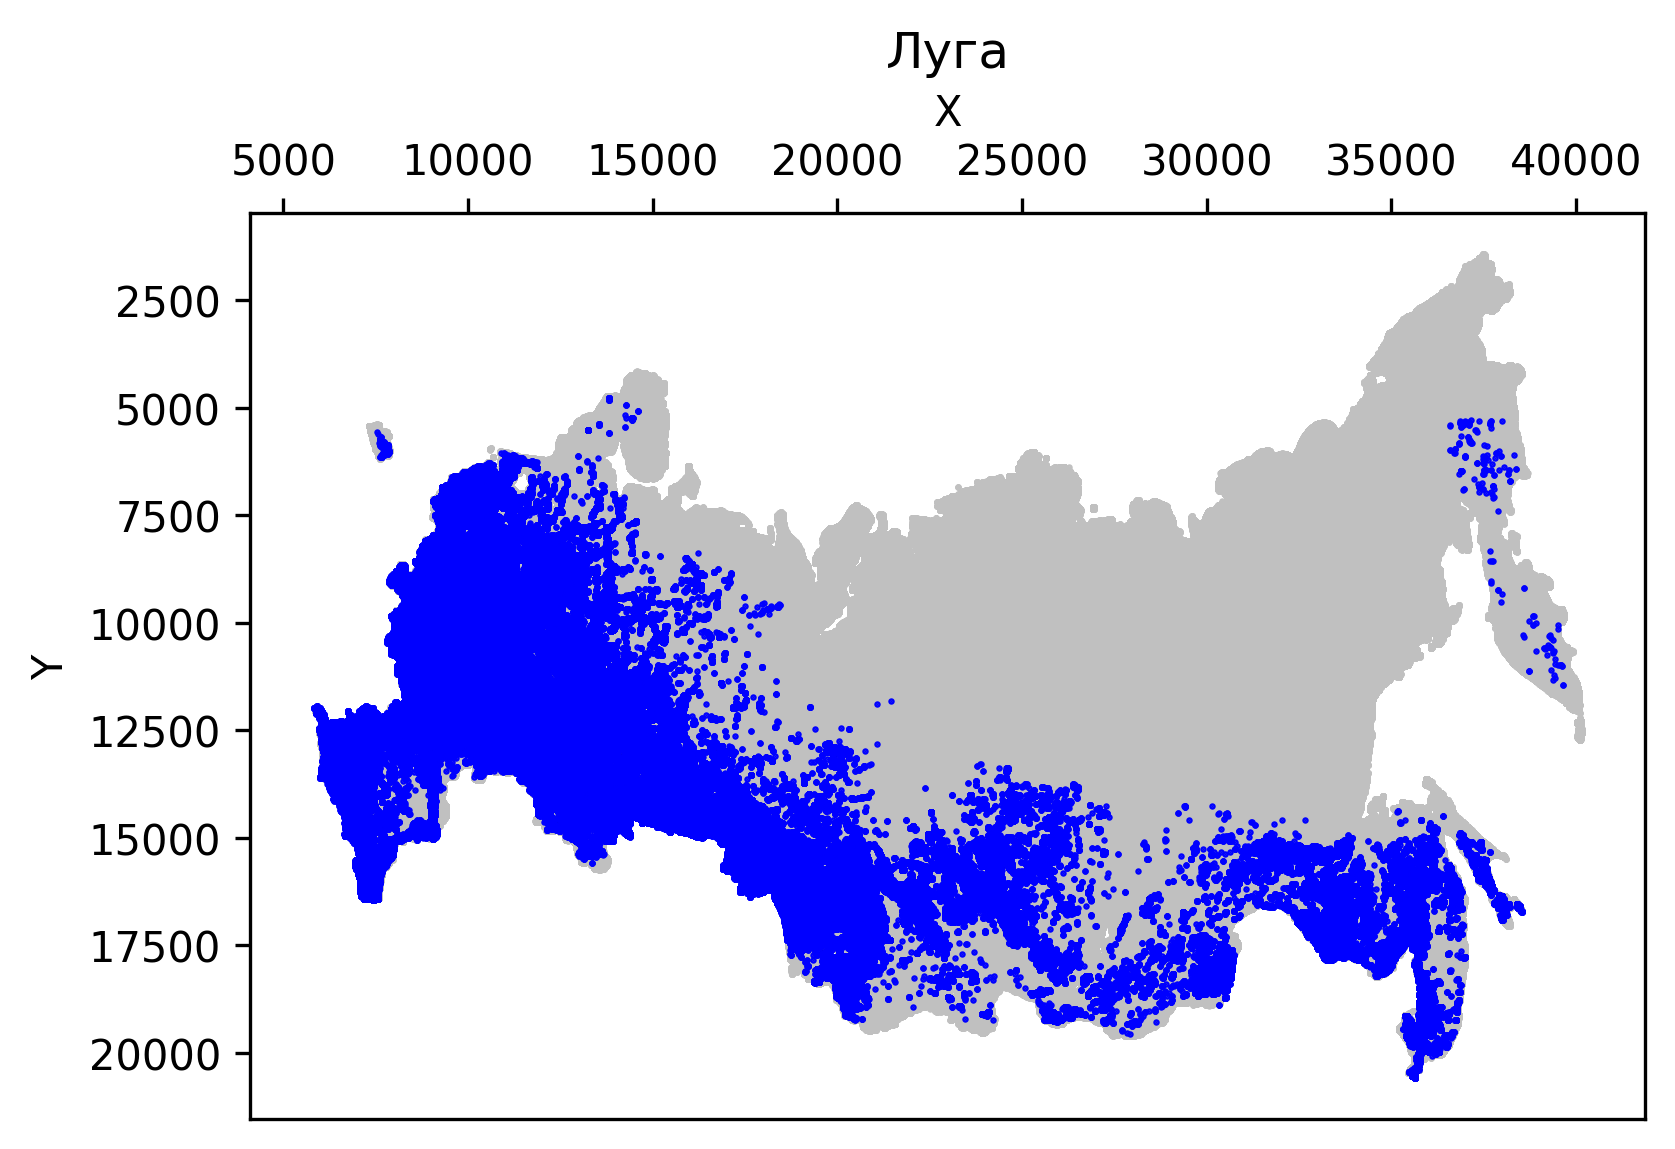
\includegraphics[]{class-8-map}
\end{figure}

\begin{figure}[H]
    \centering
    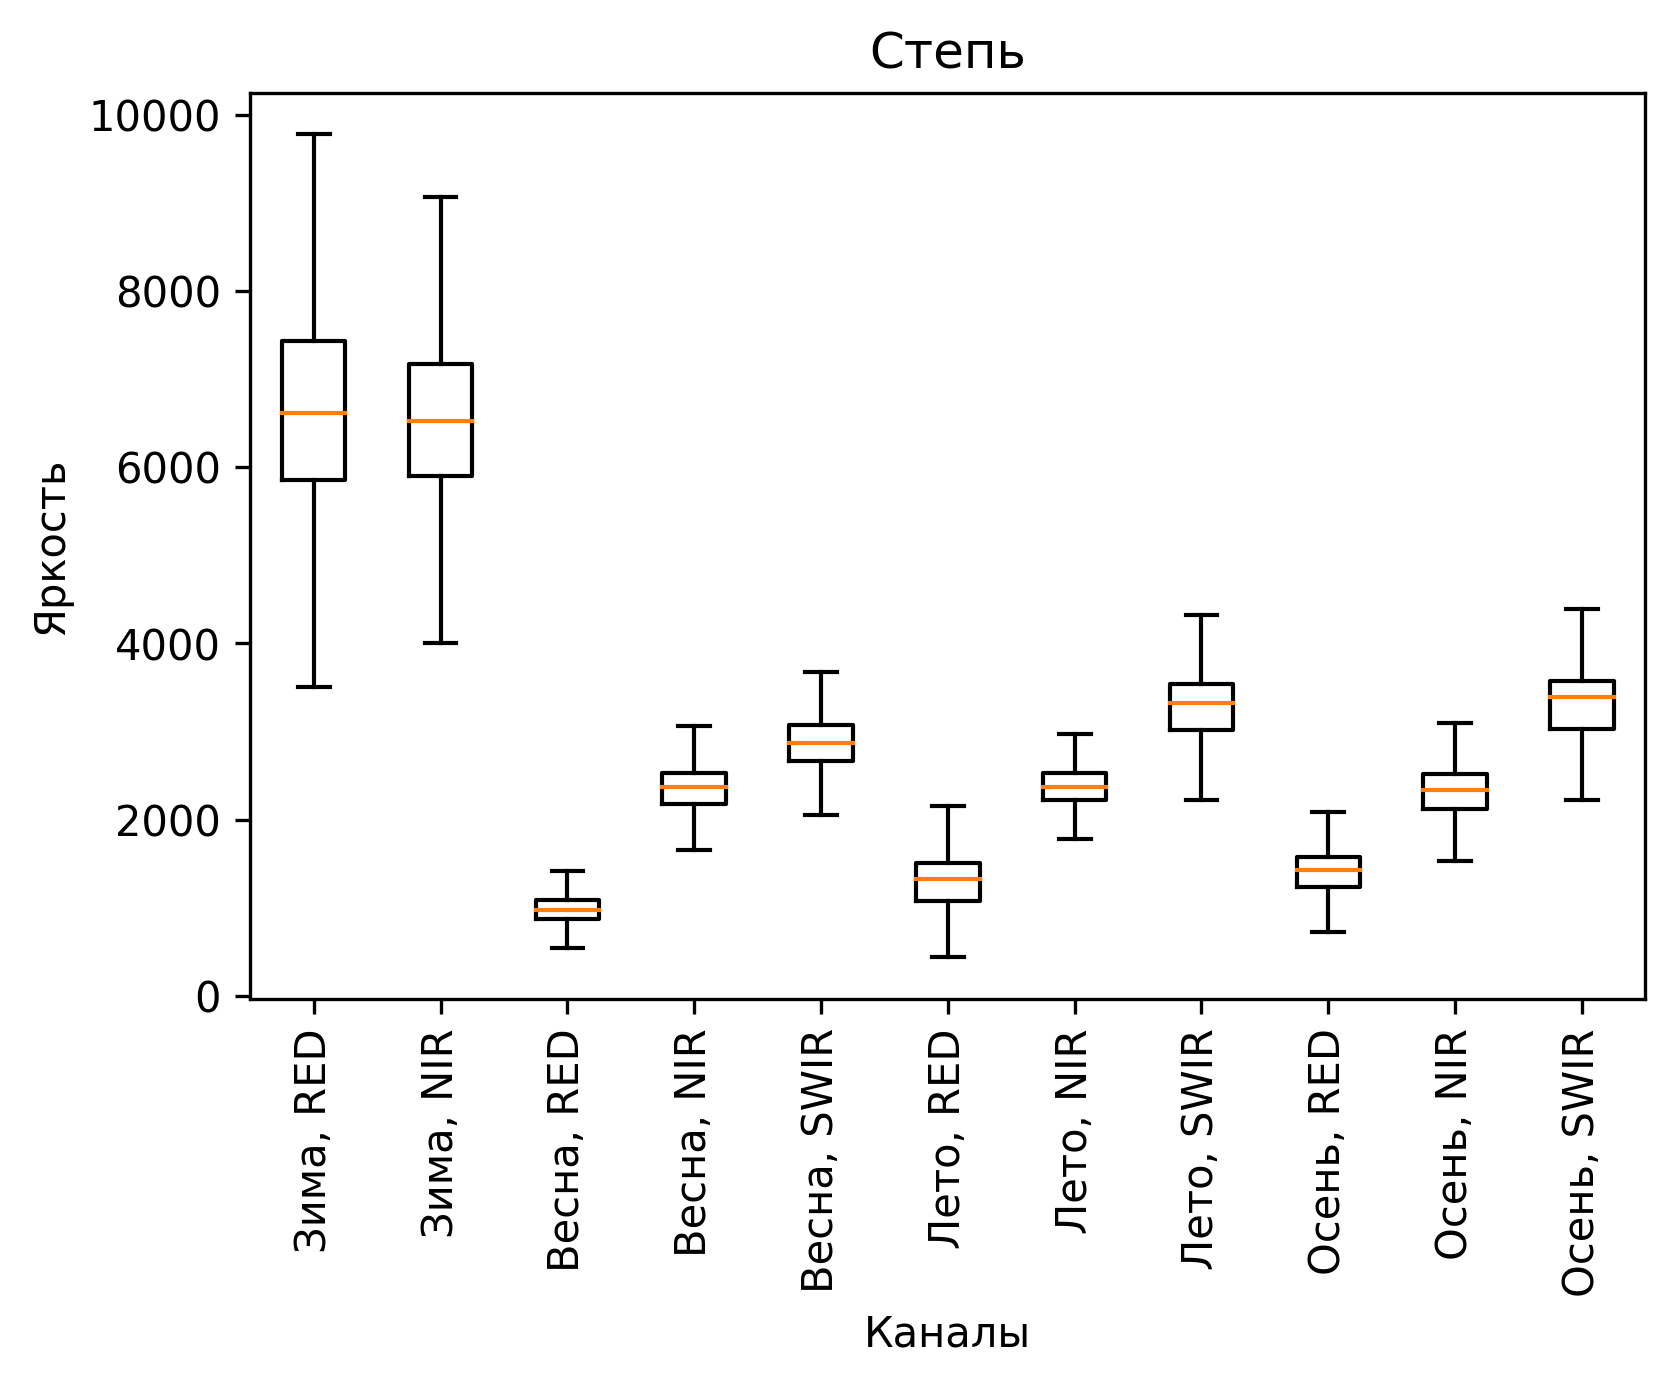
\includegraphics[]{class-14-boxplot}
    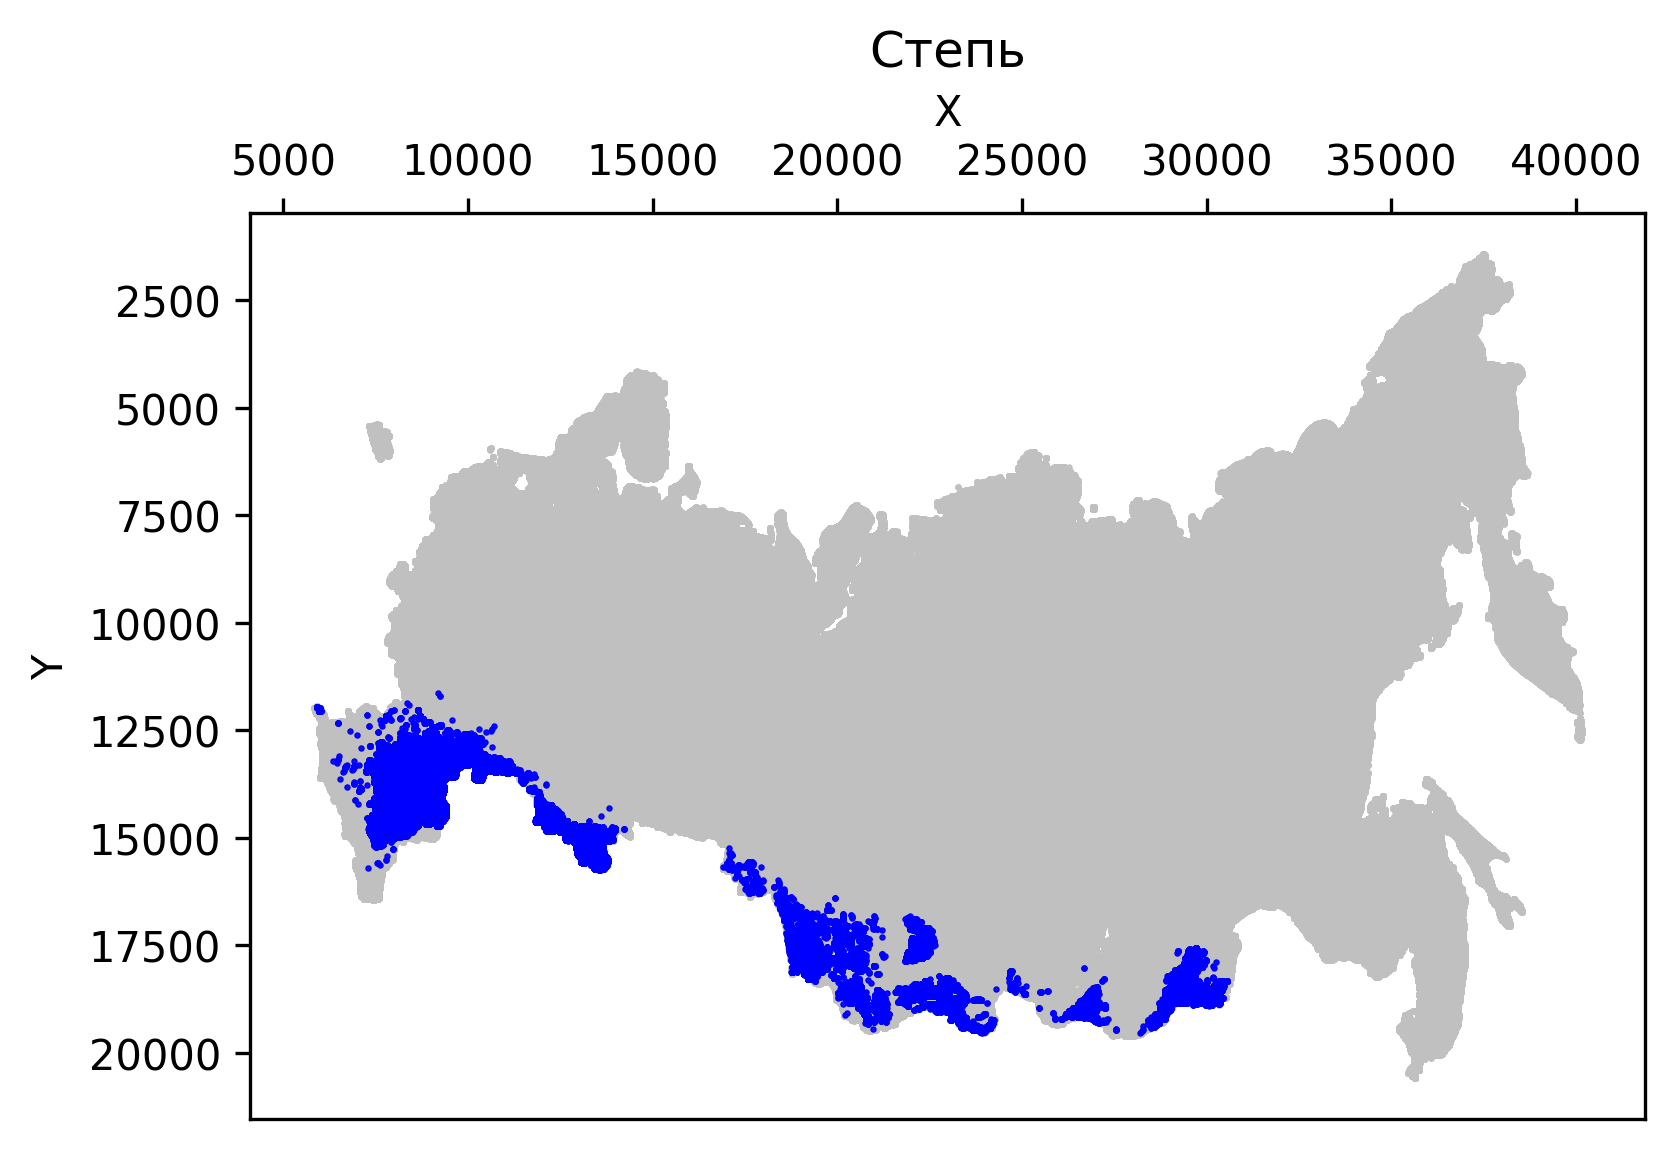
\includegraphics[]{class-14-map}
\end{figure}

\begin{figure}[H]
    \centering
    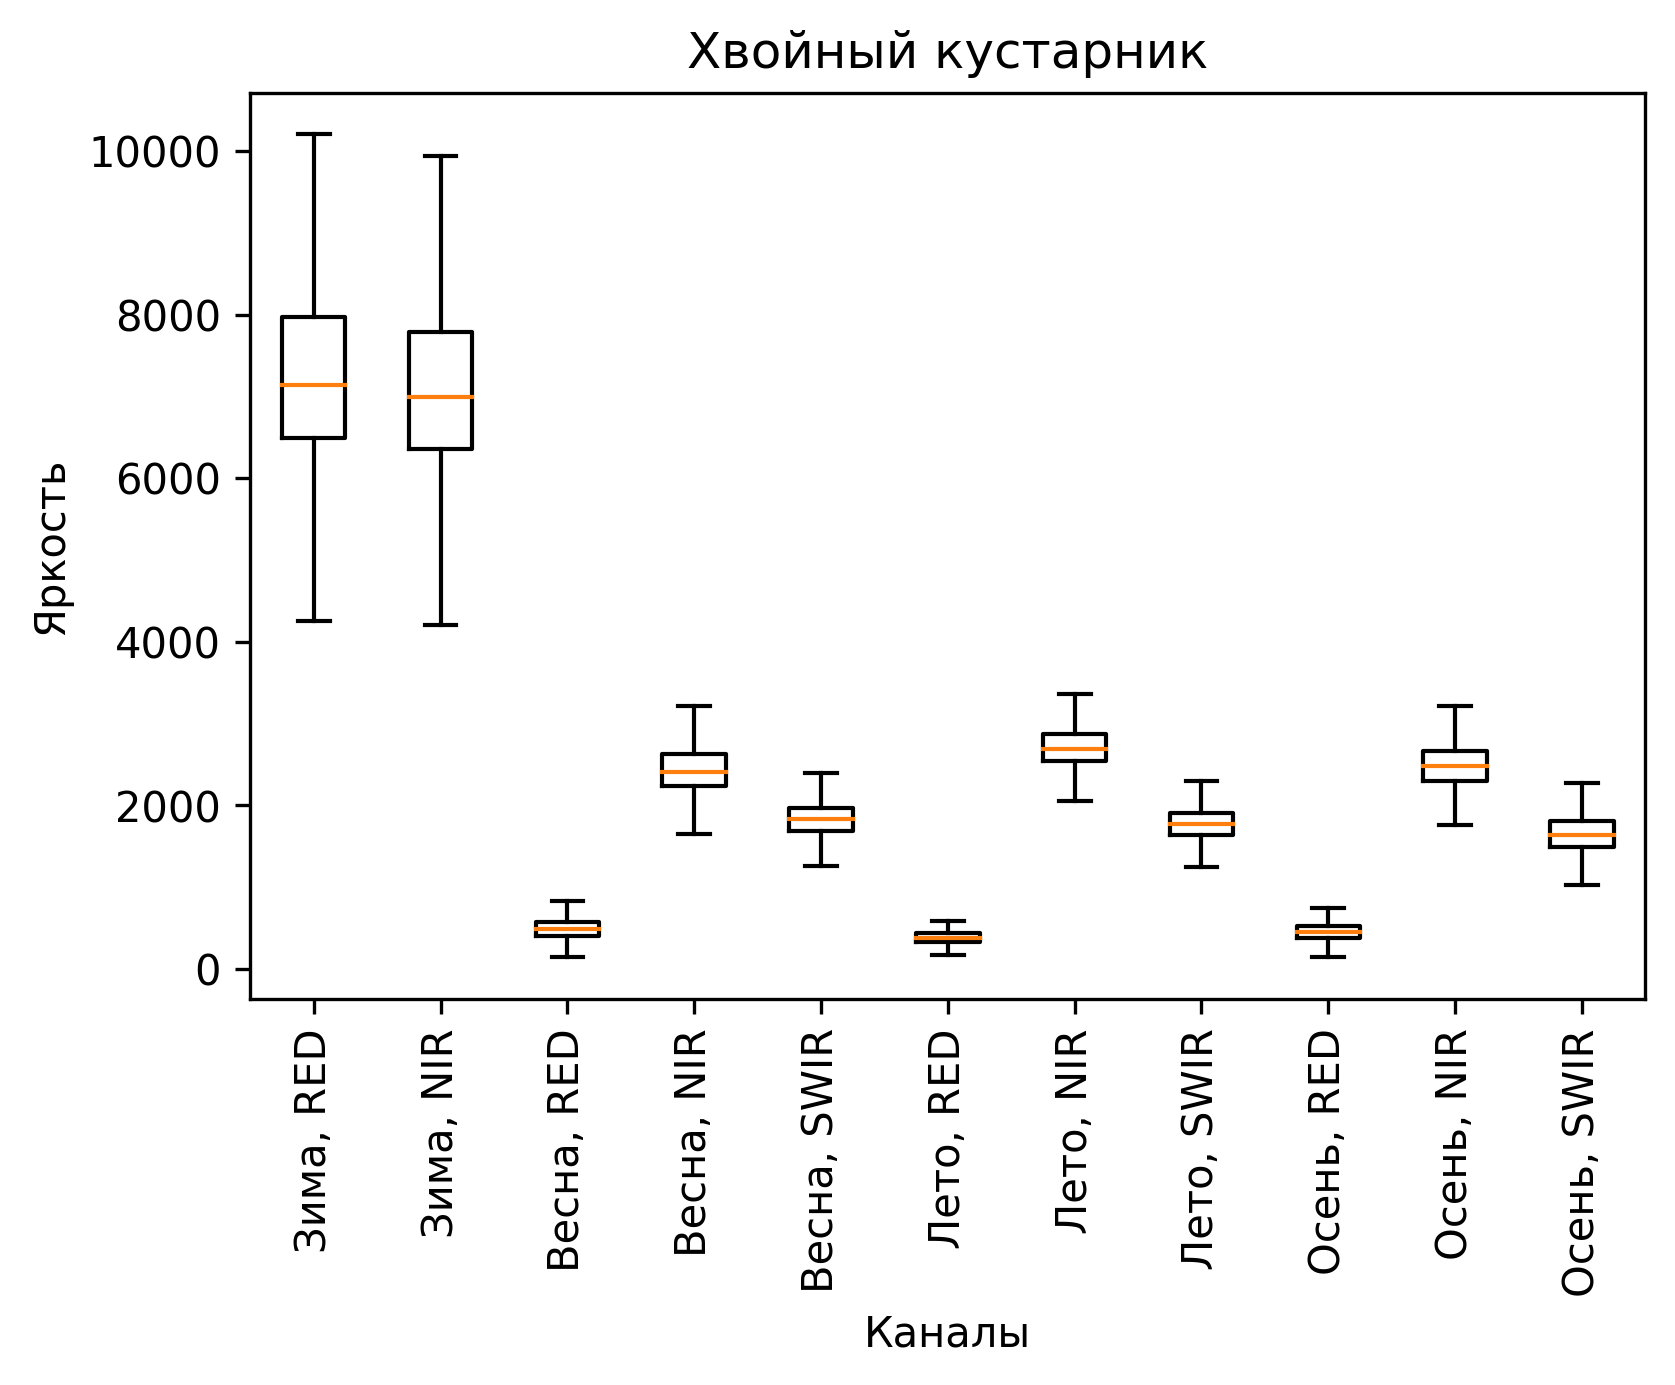
\includegraphics[]{class-5-boxplot}
    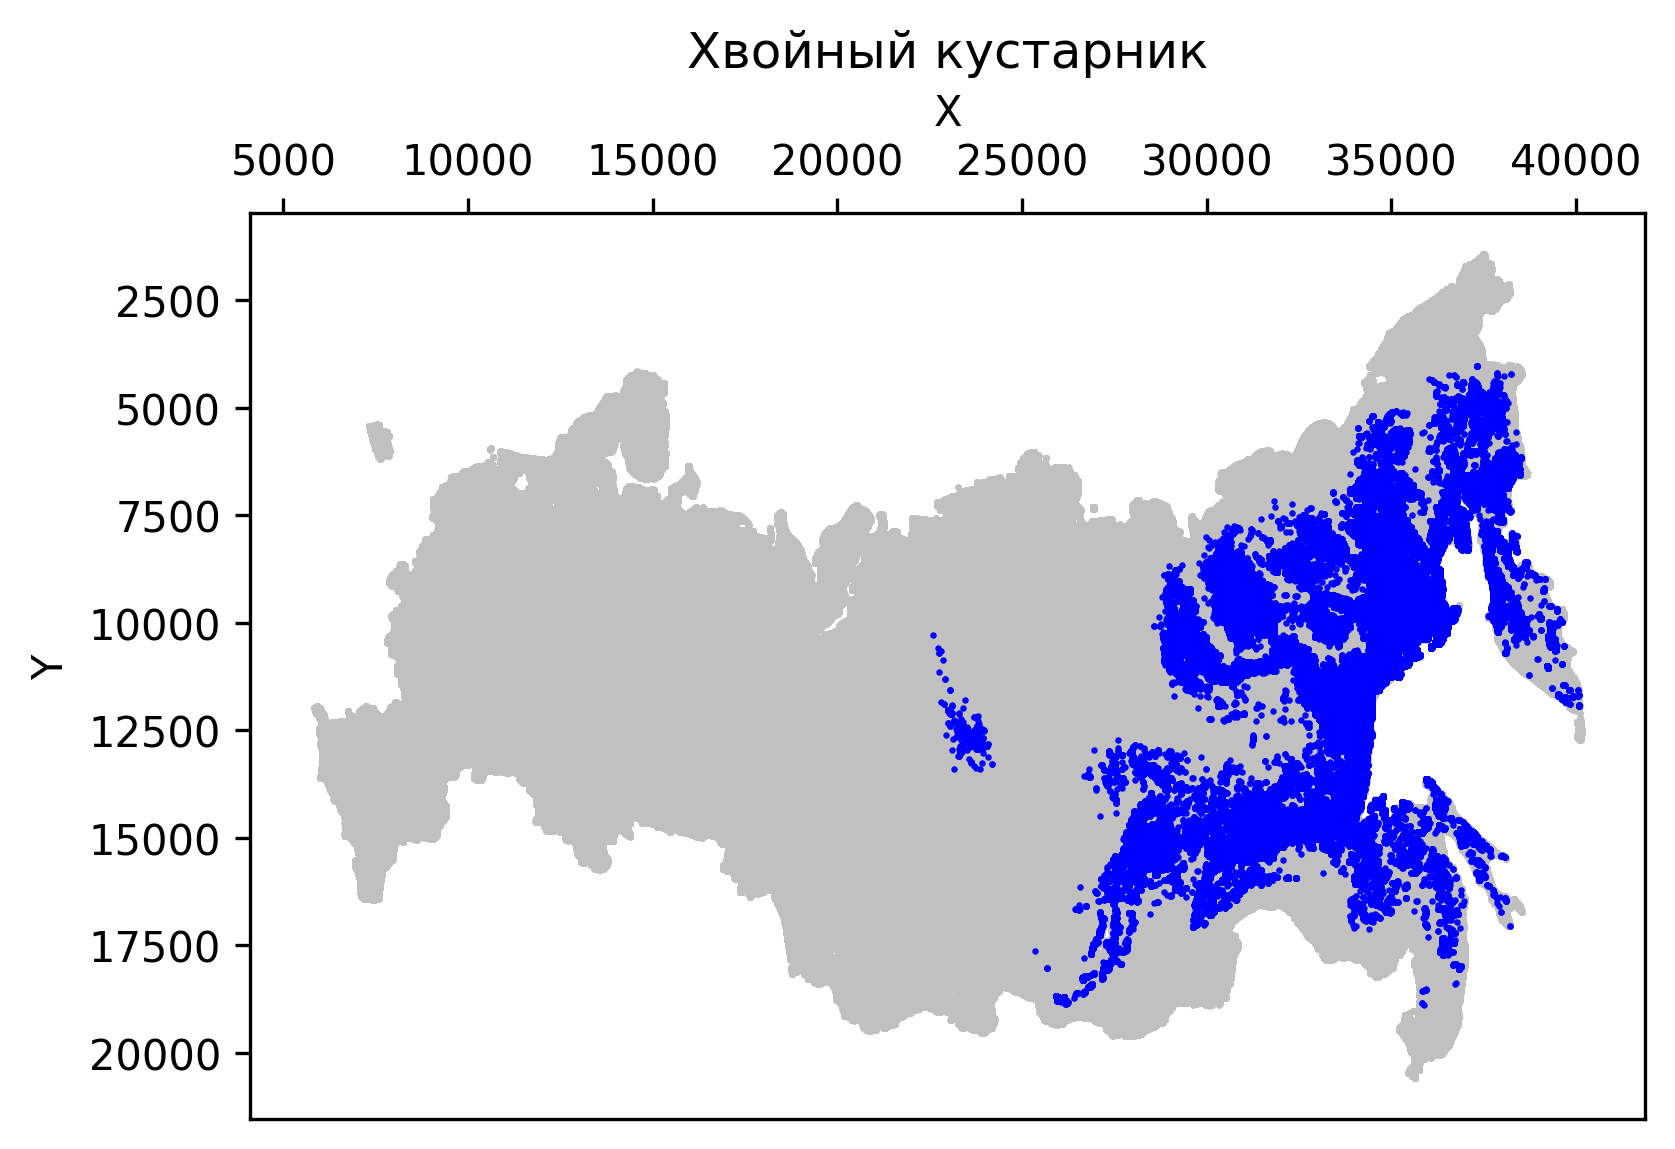
\includegraphics[]{class-5-map}
\end{figure}

\begin{figure}[H]
    \centering
    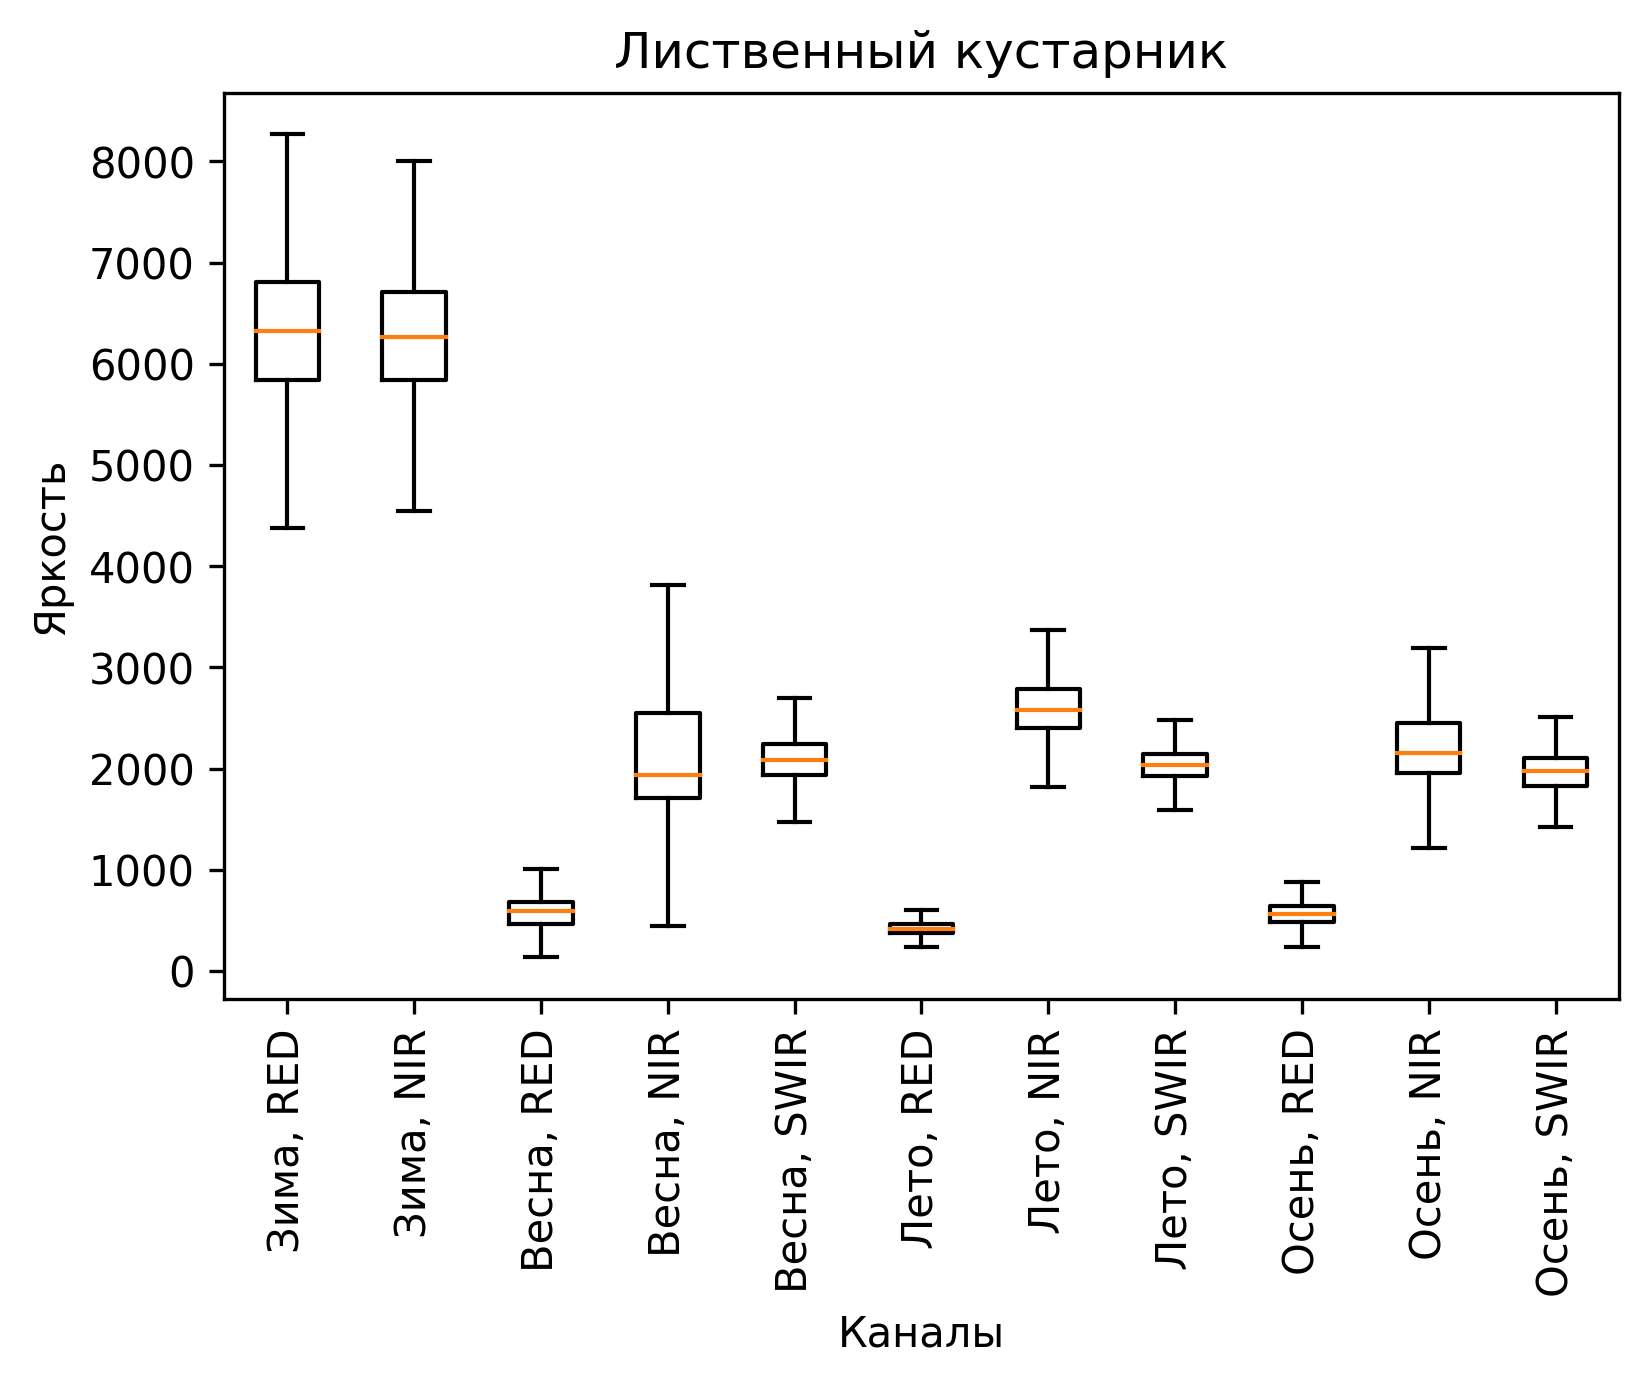
\includegraphics[]{class-9-boxplot}
    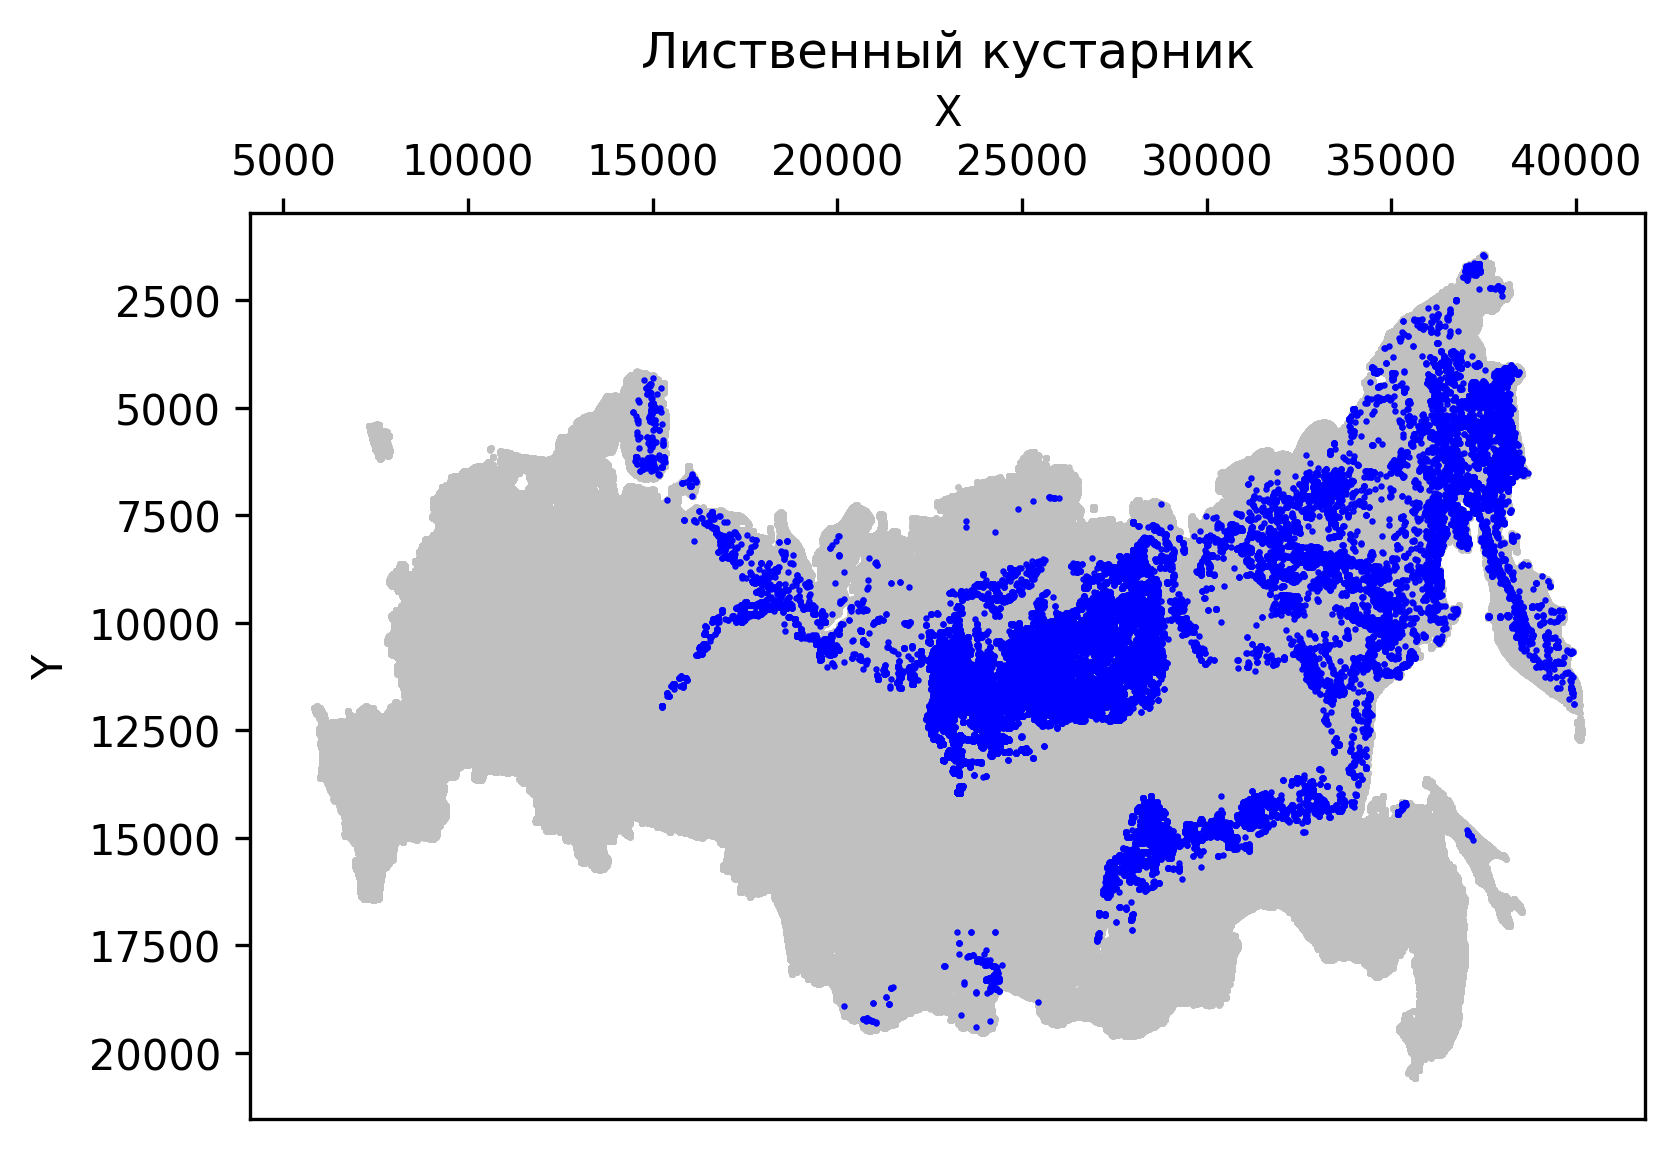
\includegraphics[]{class-9-map}
\end{figure}

\begin{figure}[H]
    \centering
    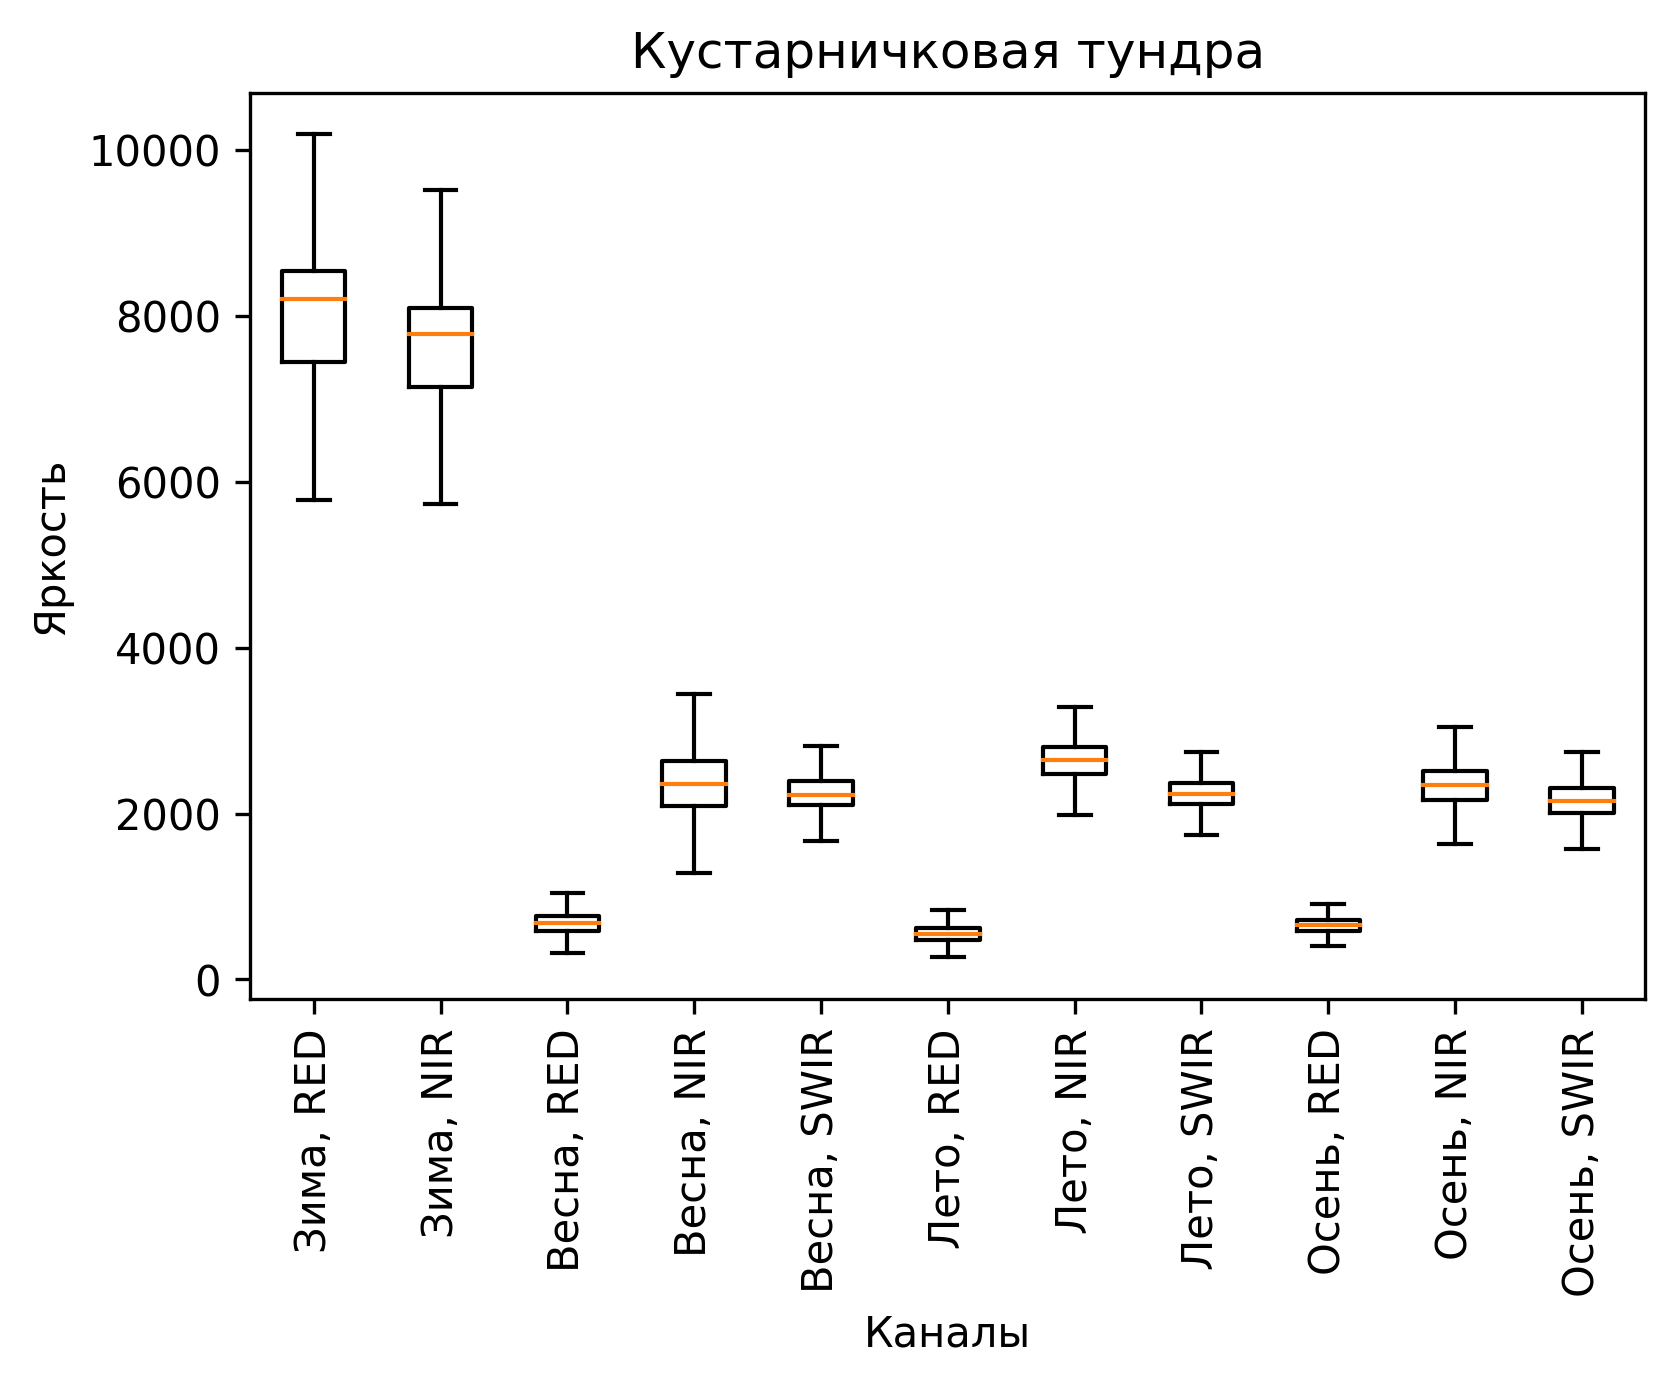
\includegraphics[]{class-18-boxplot}
    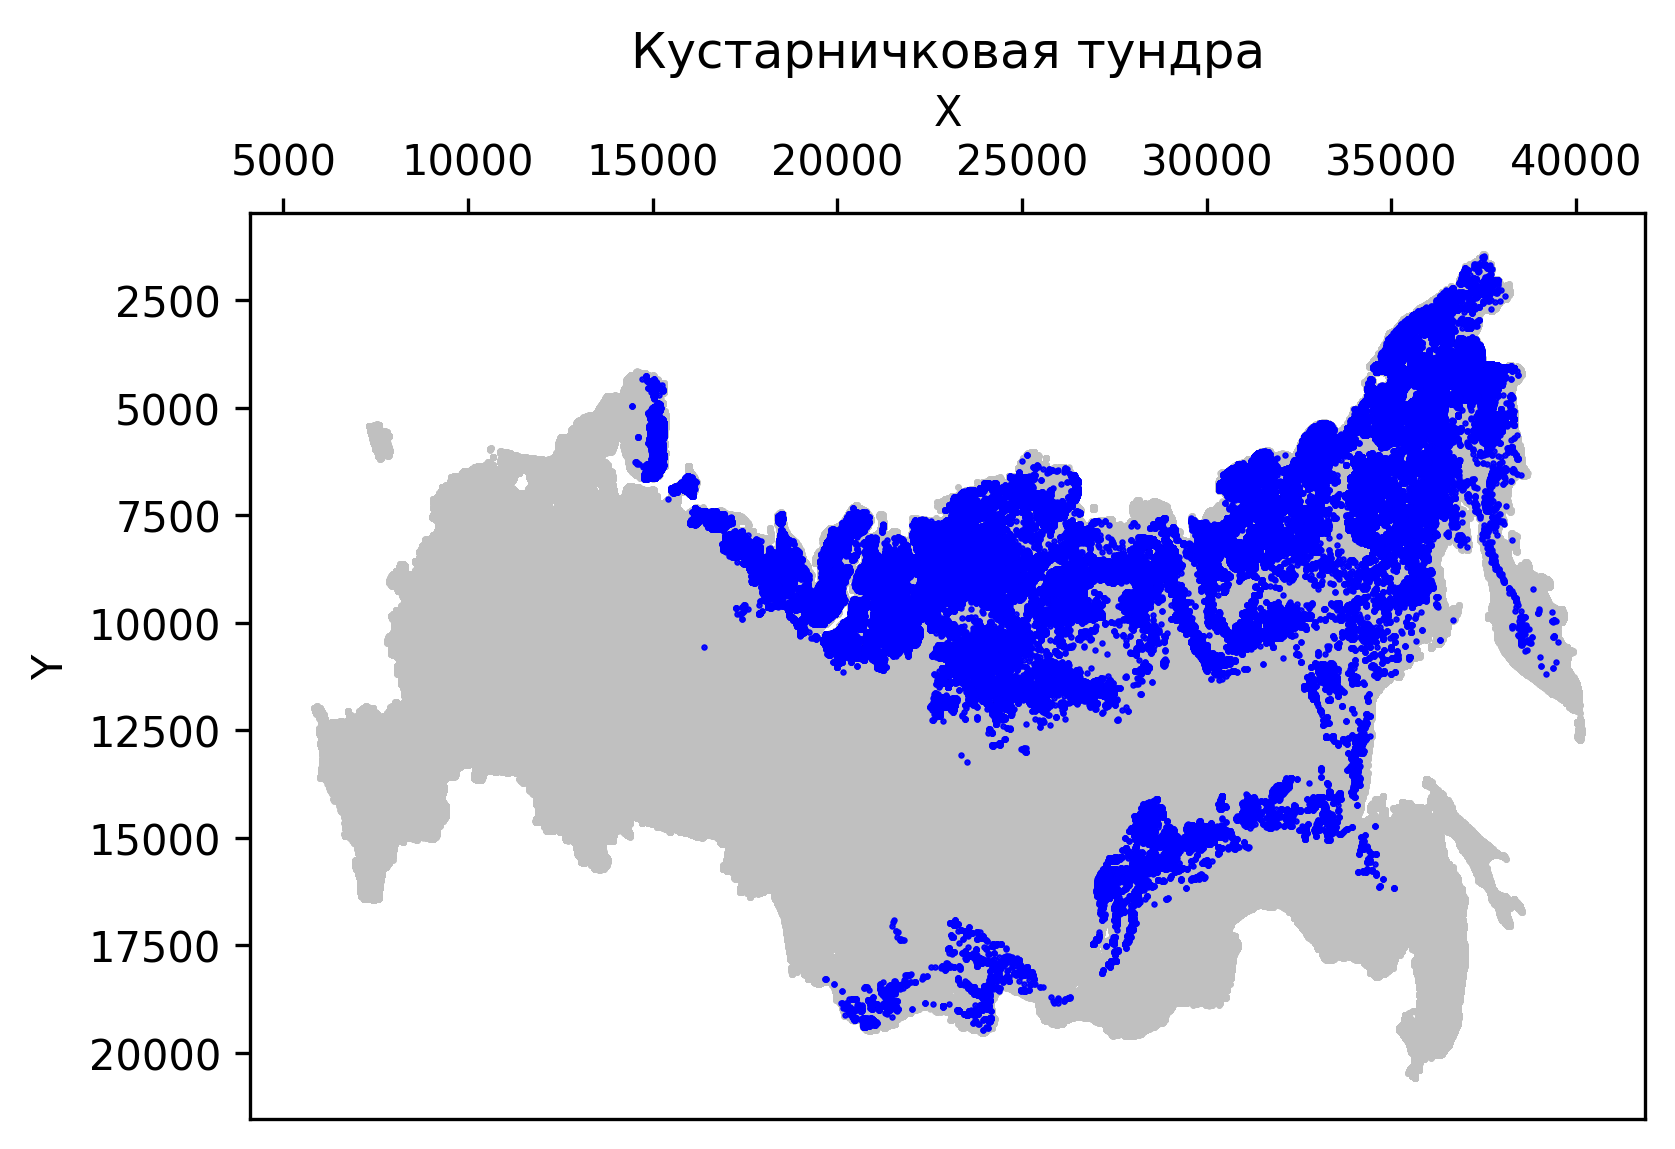
\includegraphics[]{class-18-map}
\end{figure}

\begin{figure}[H]
    \centering
    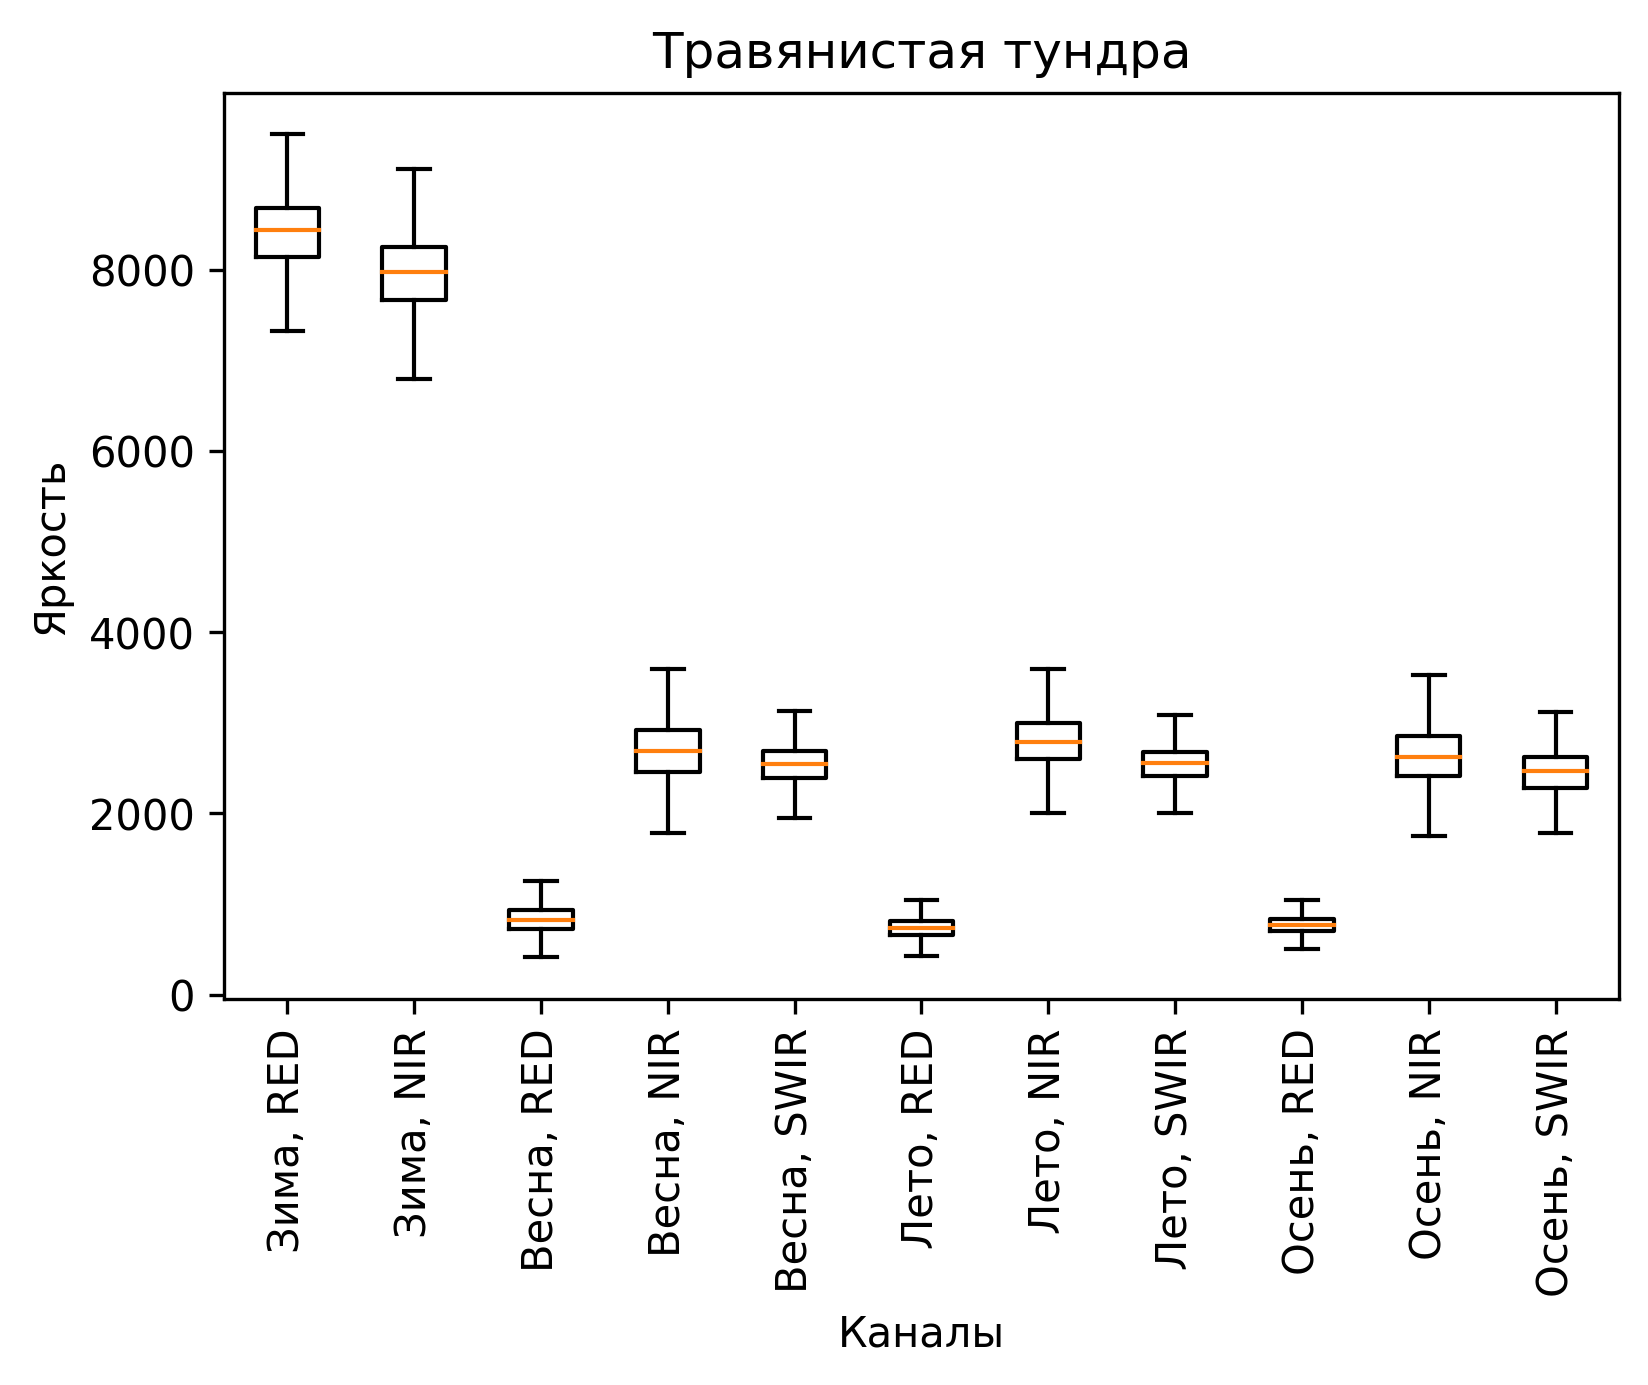
\includegraphics[]{class-17-boxplot}
    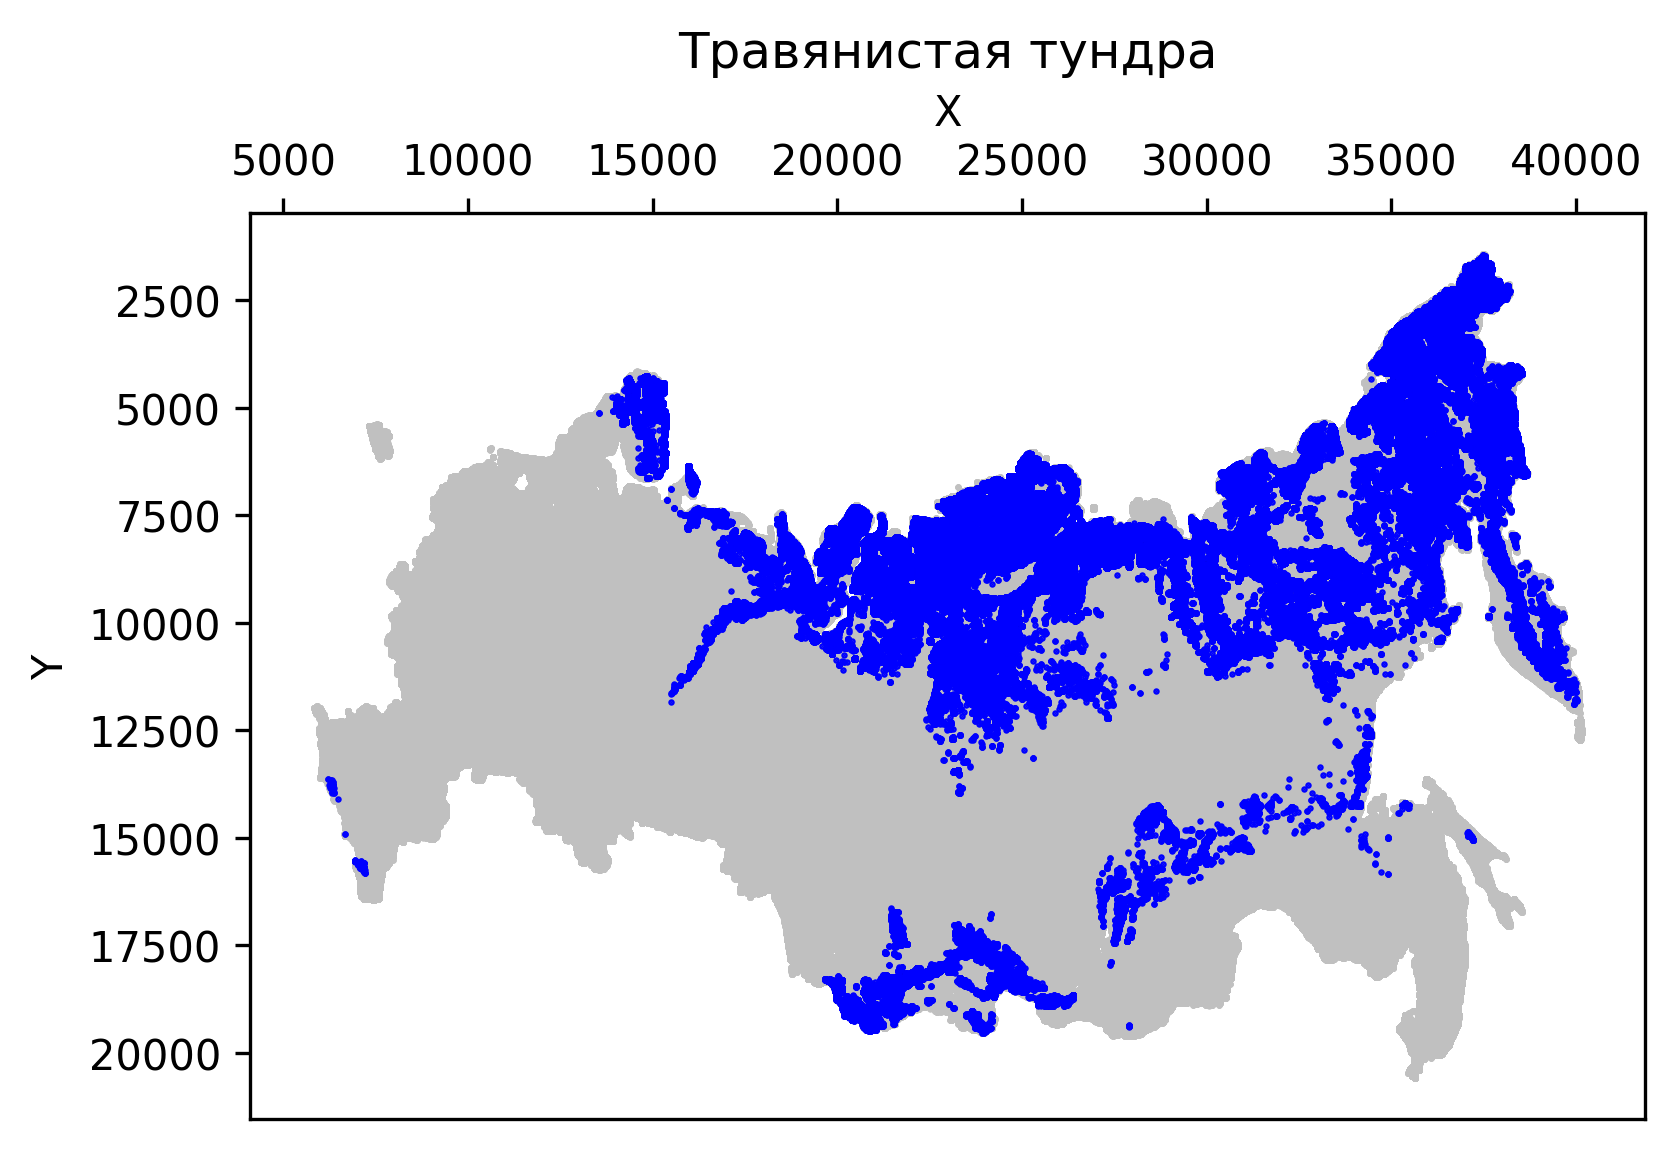
\includegraphics[]{class-17-map}
\end{figure}

\begin{figure}[H]
    \centering
    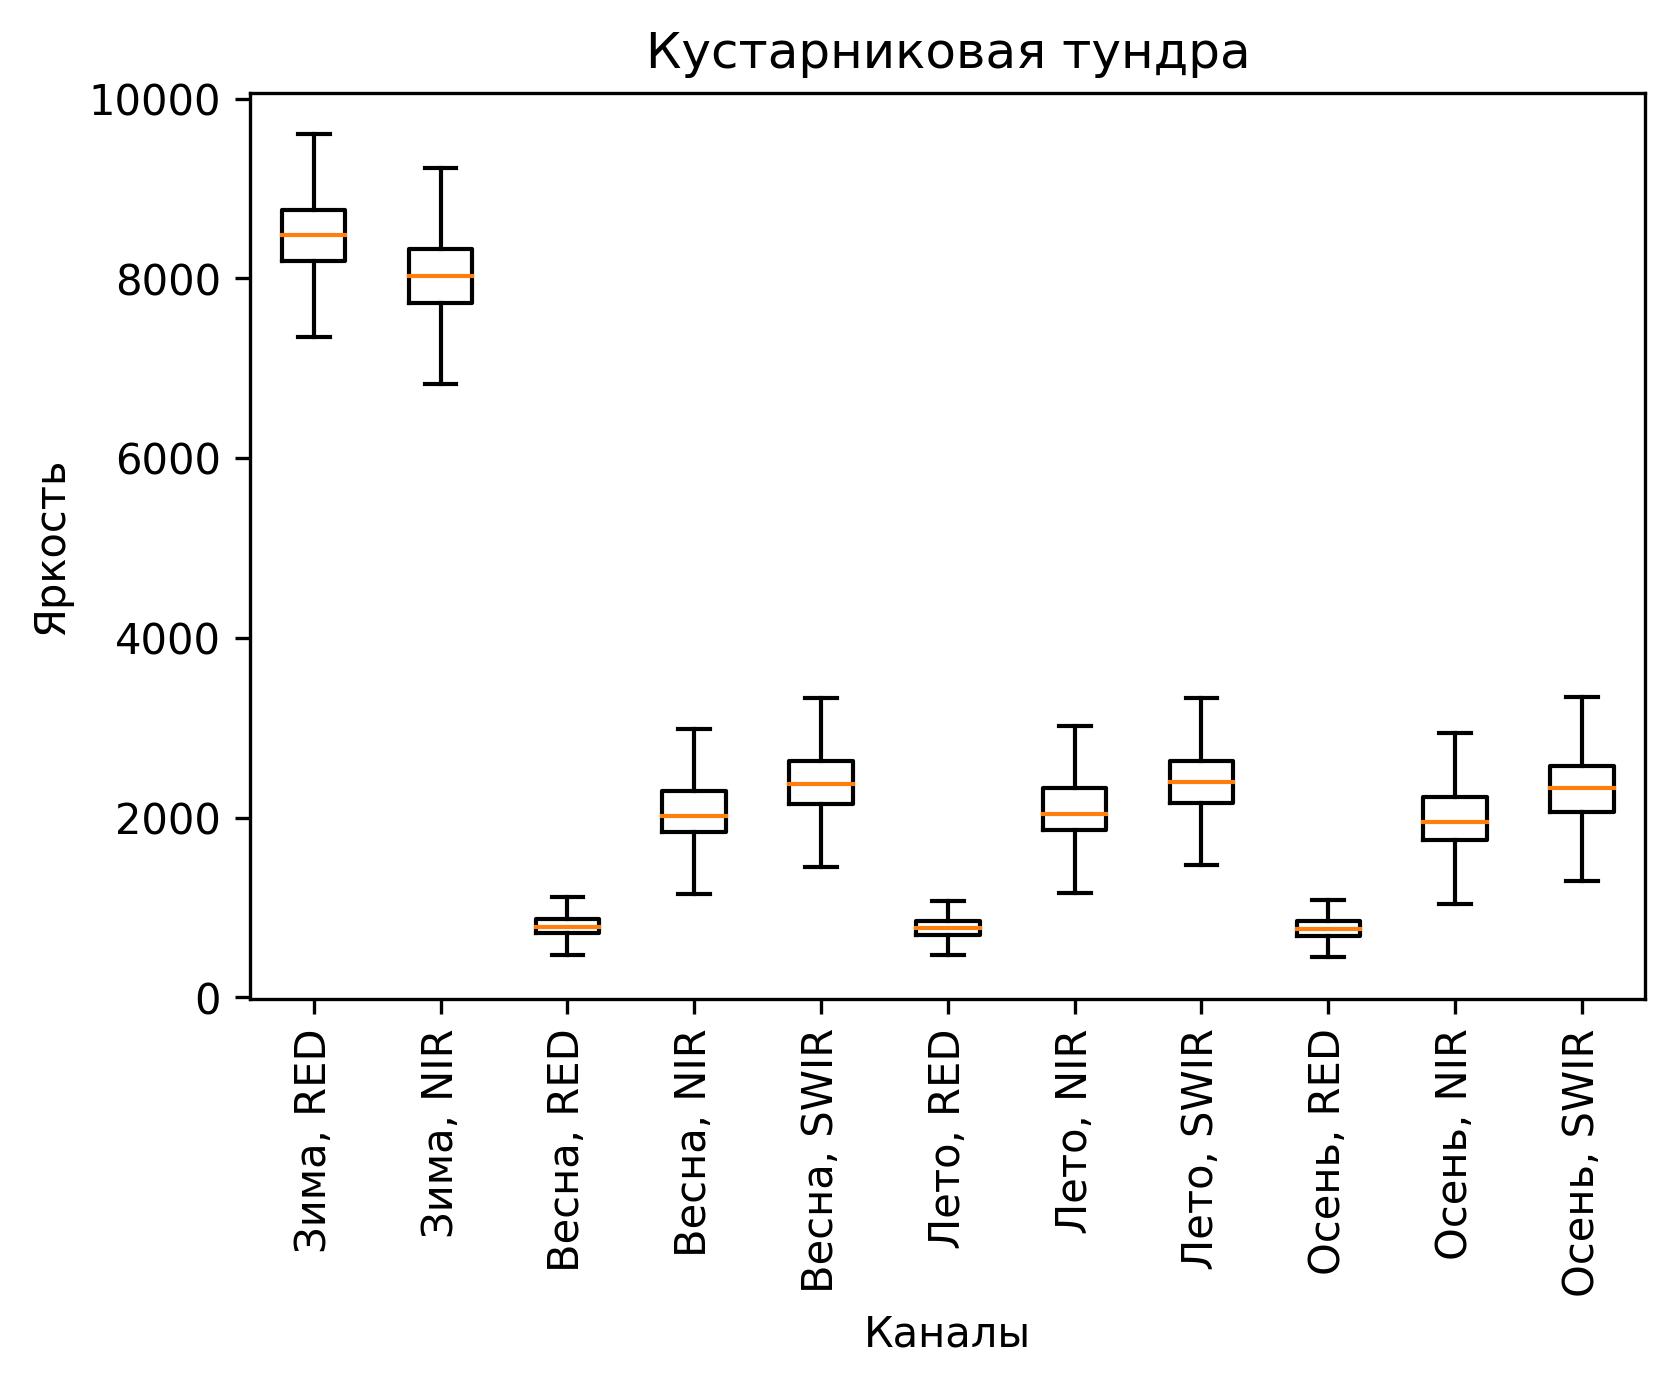
\includegraphics[]{class-16-boxplot}
    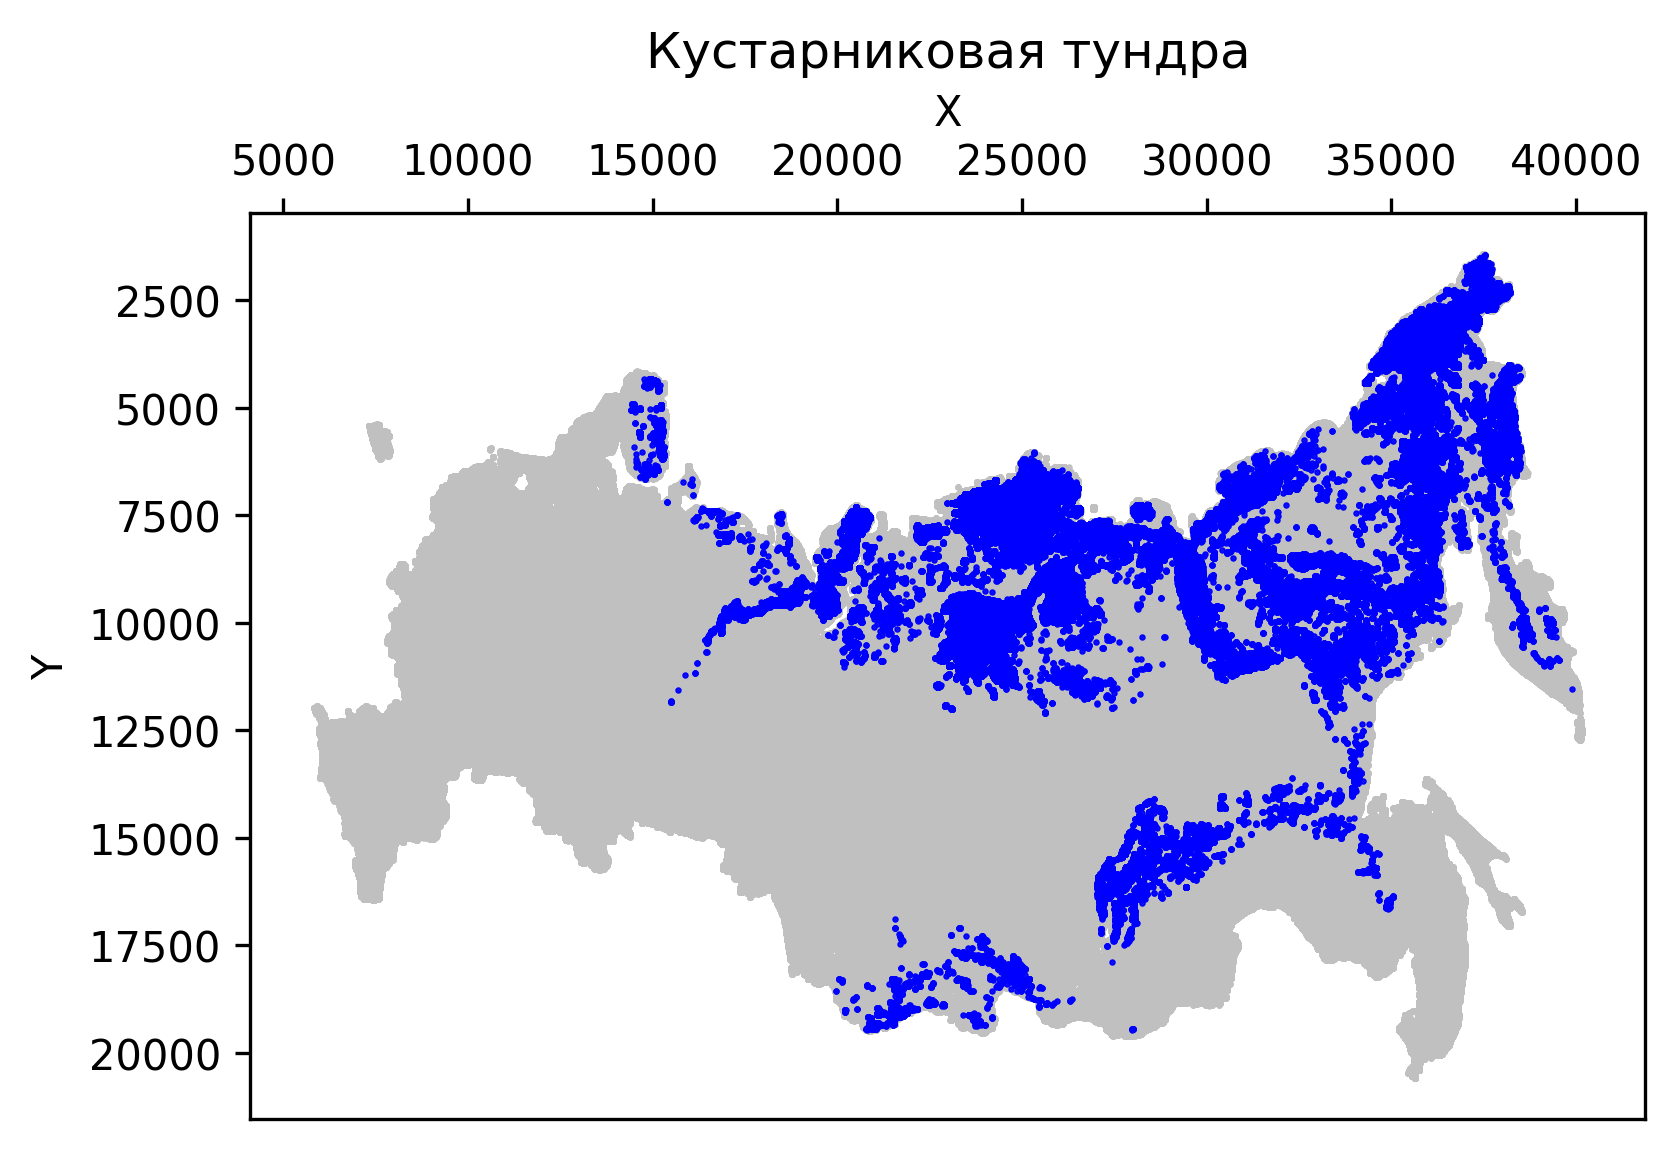
\includegraphics[]{class-16-map}
\end{figure}

\begin{figure}[H]
    \centering
    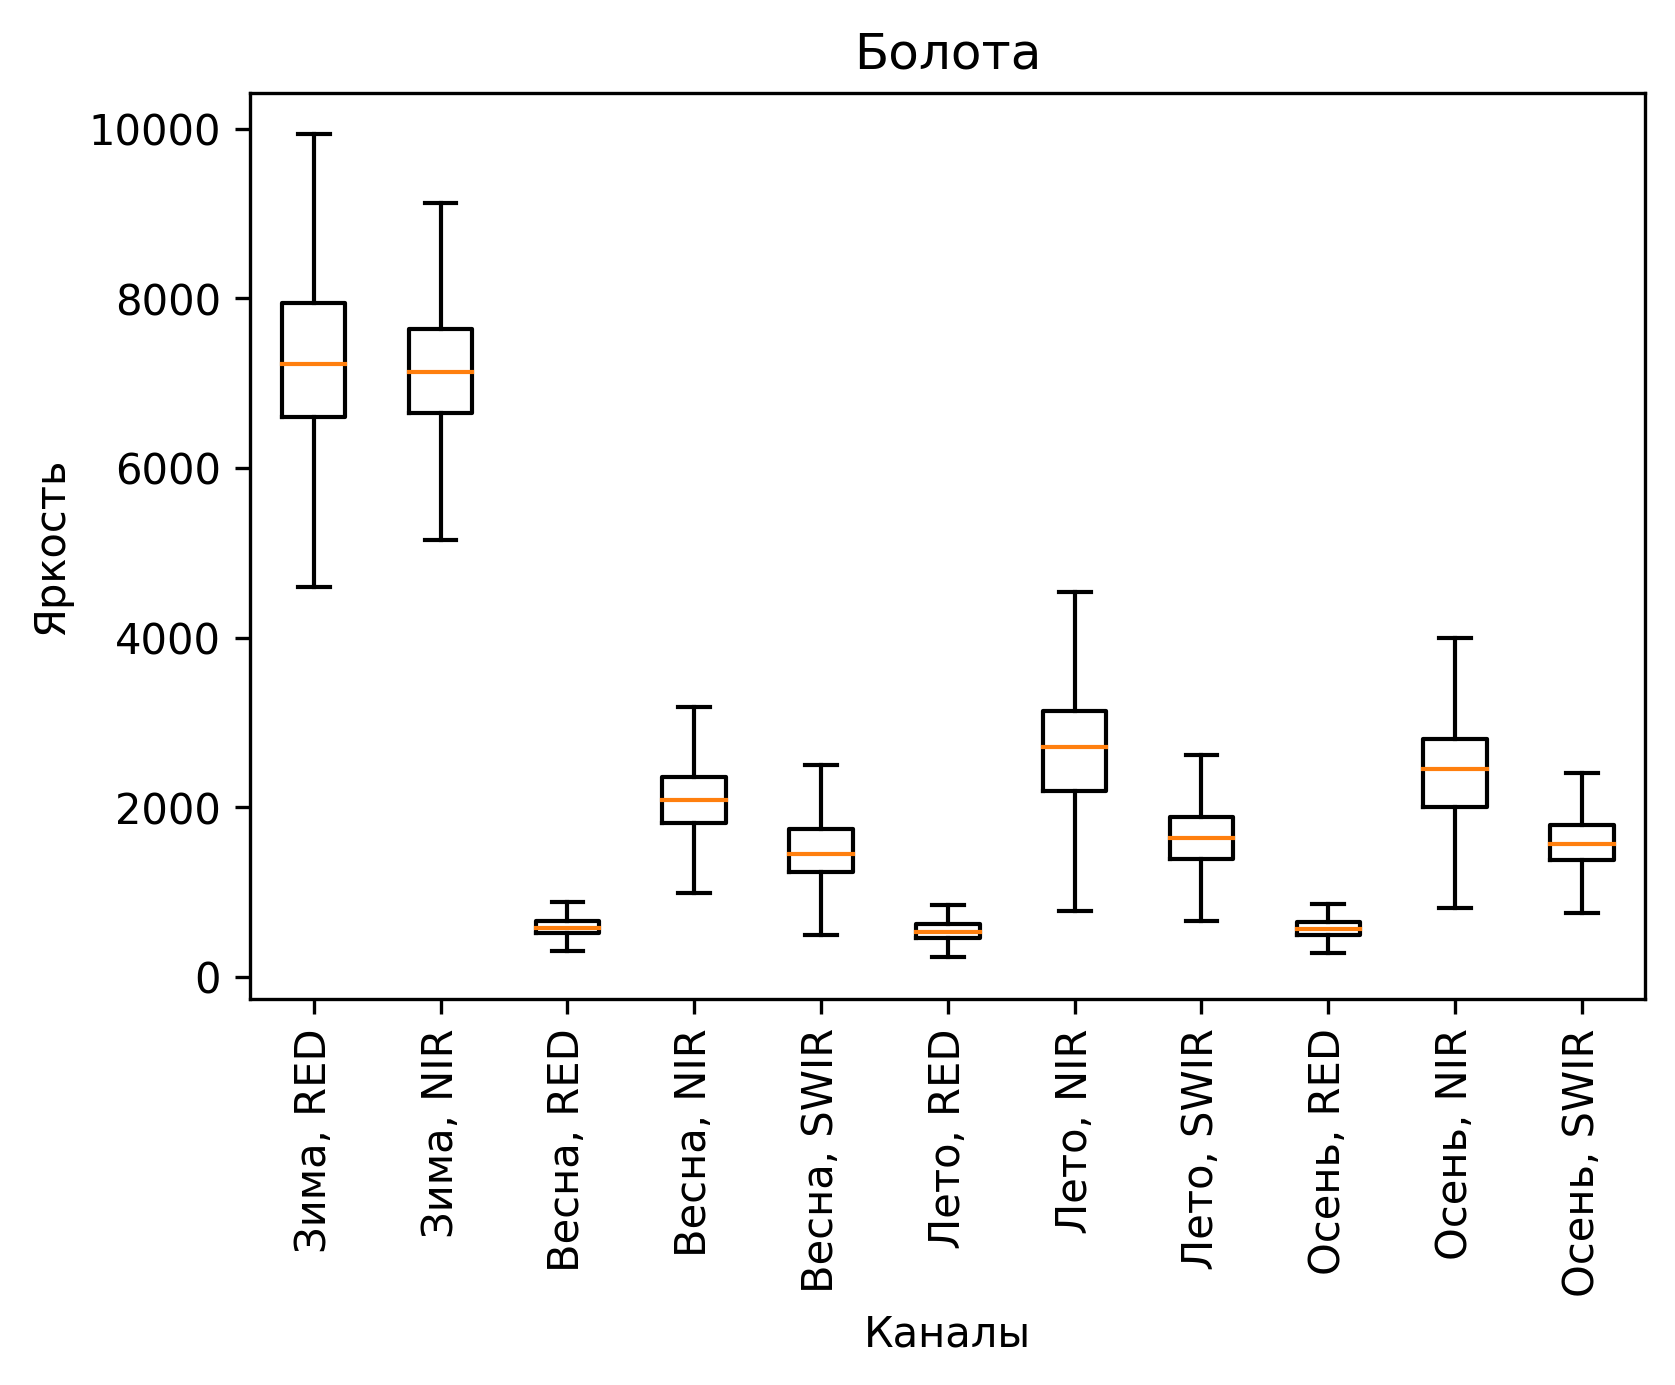
\includegraphics[]{class-6-boxplot}
    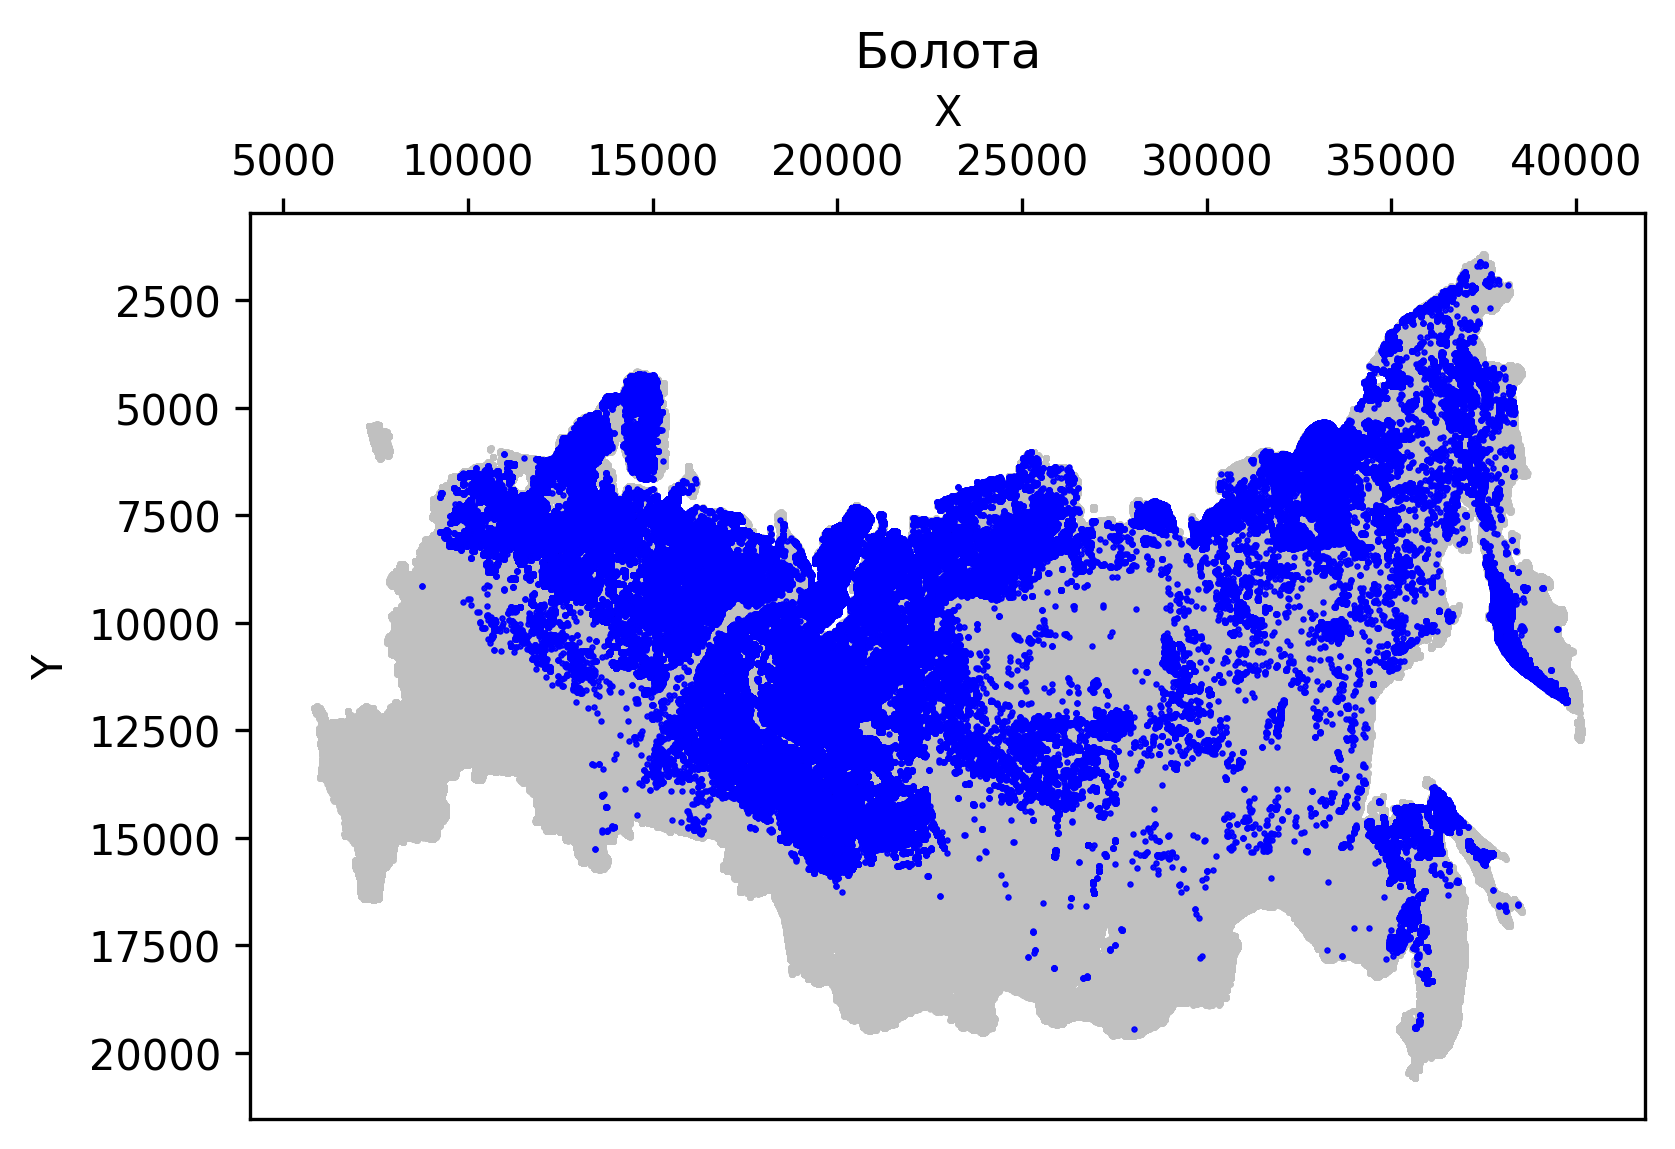
\includegraphics[]{class-6-map}
\end{figure}

\begin{figure}[H]
    \centering
    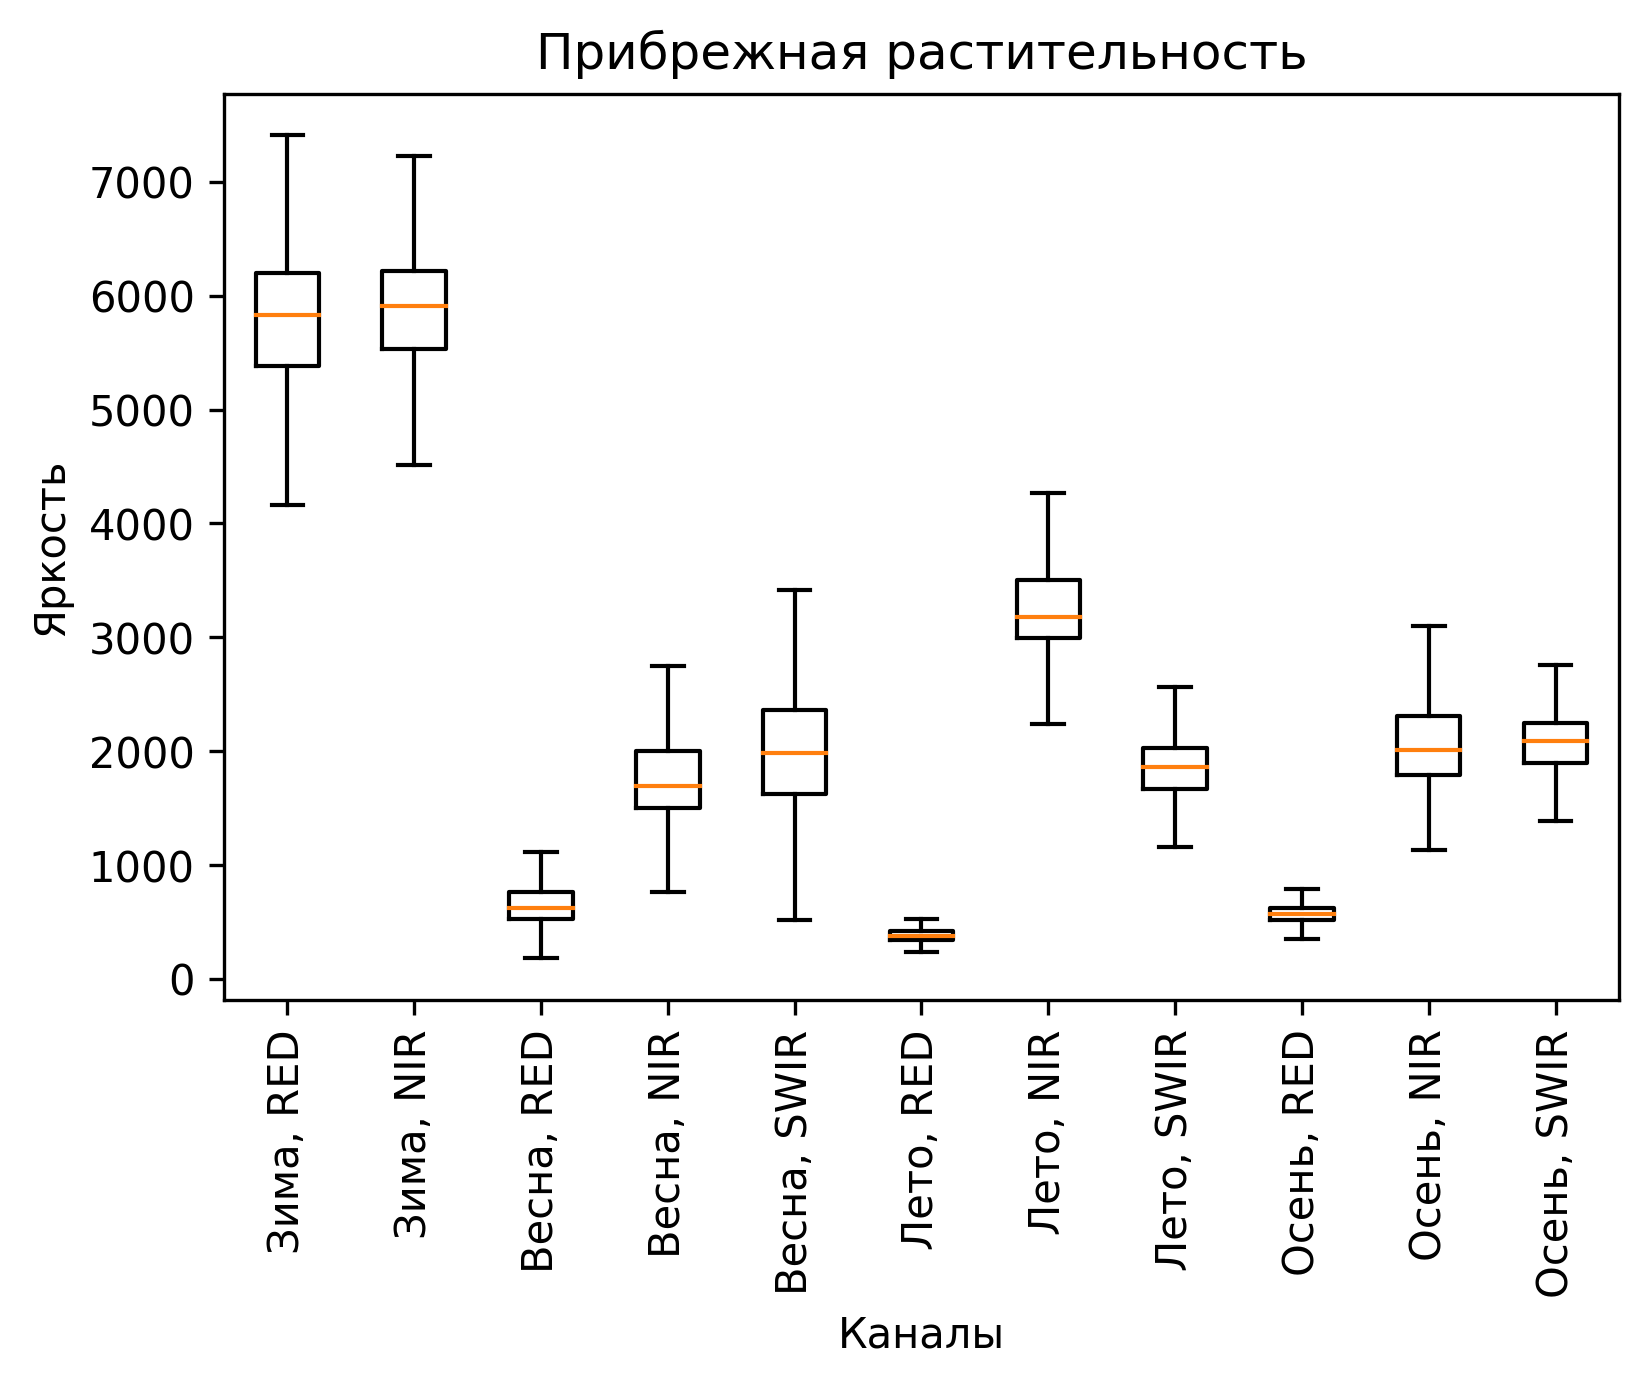
\includegraphics[]{class-15-boxplot}
    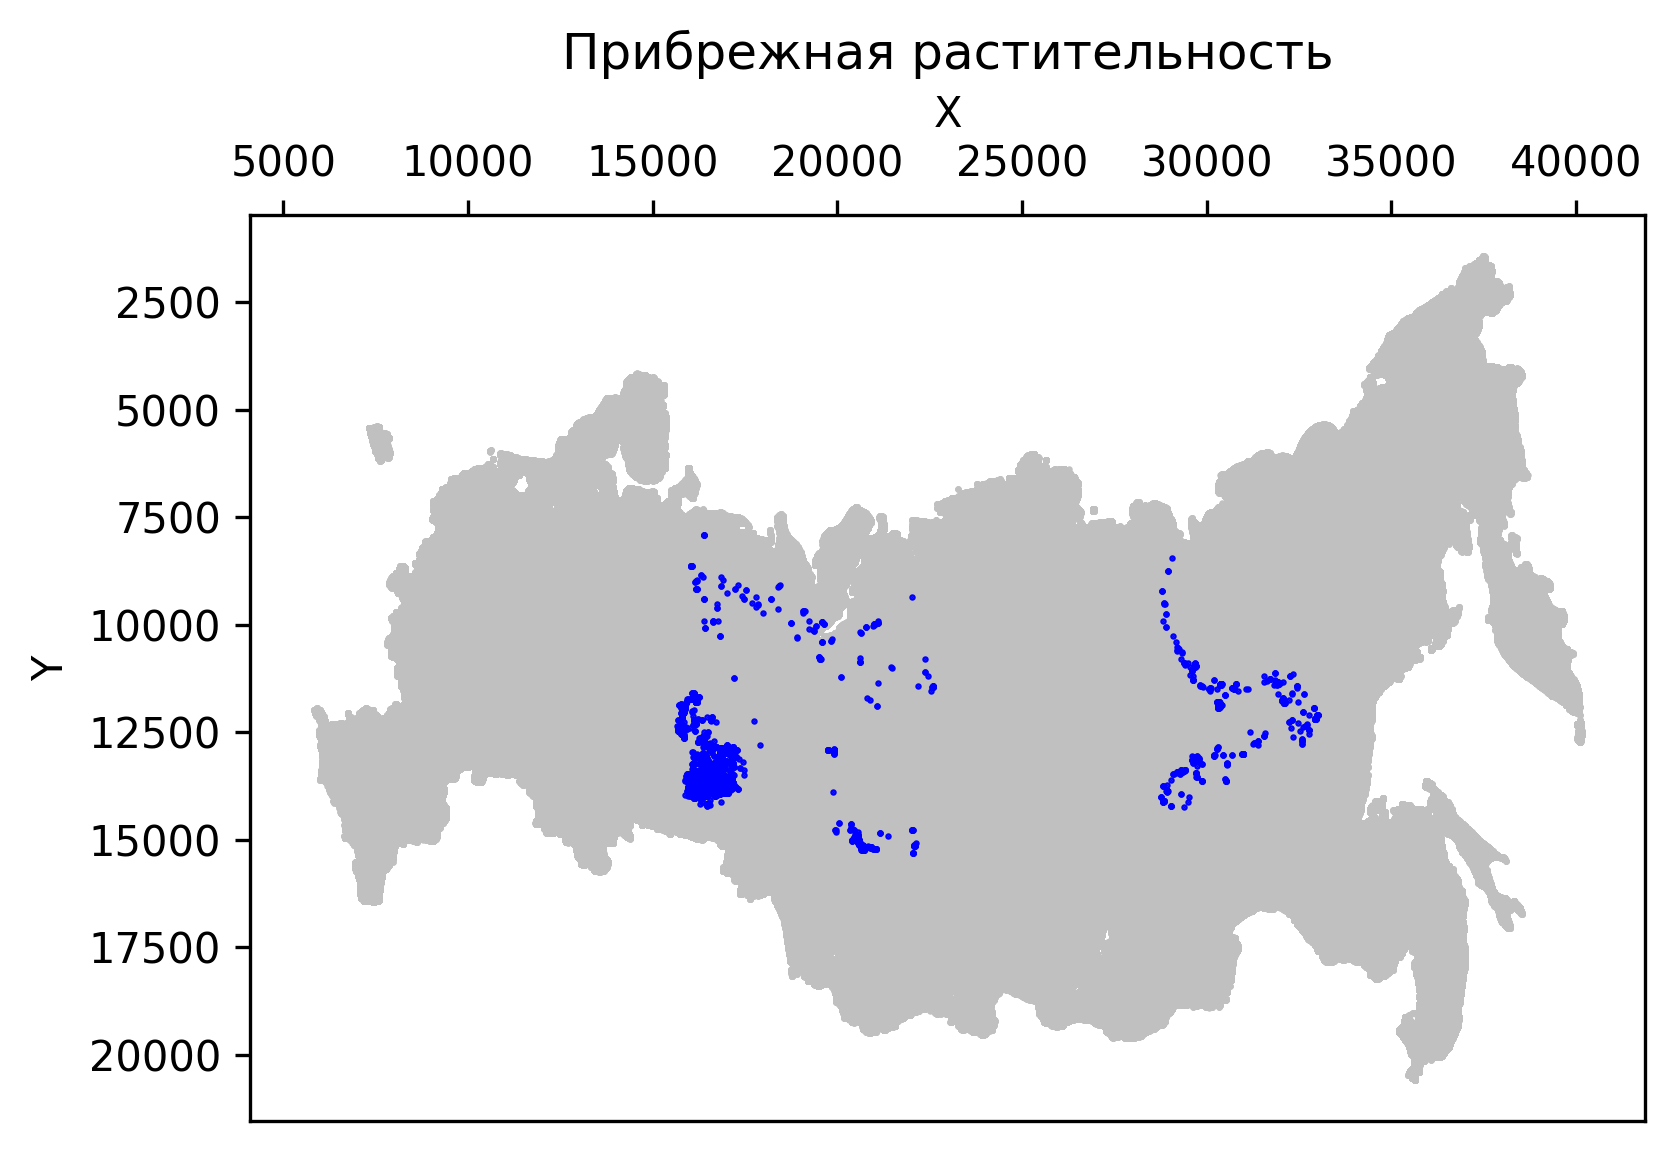
\includegraphics[]{class-15-map}
\end{figure}

\begin{figure}[H]
    \centering
    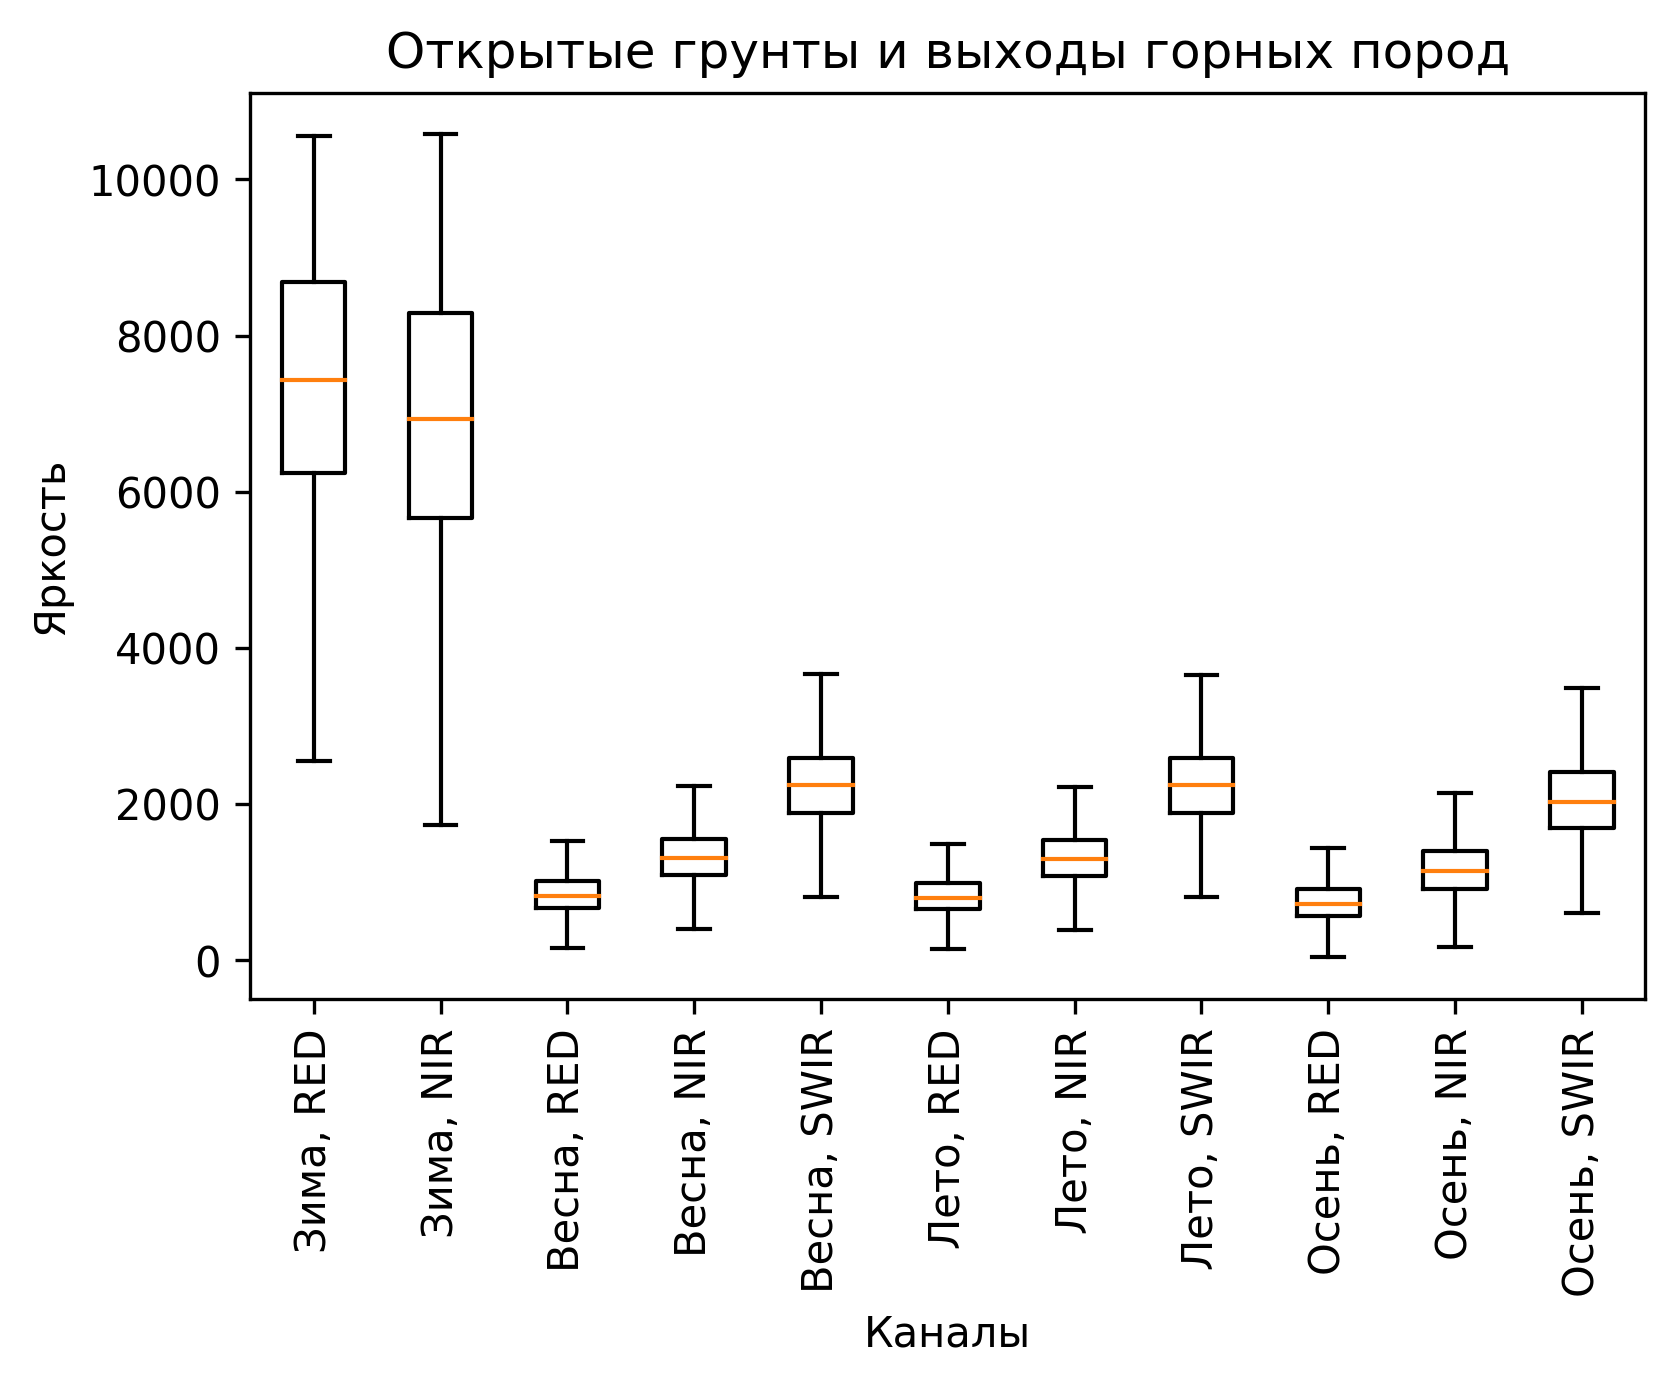
\includegraphics[]{class-13-boxplot}
    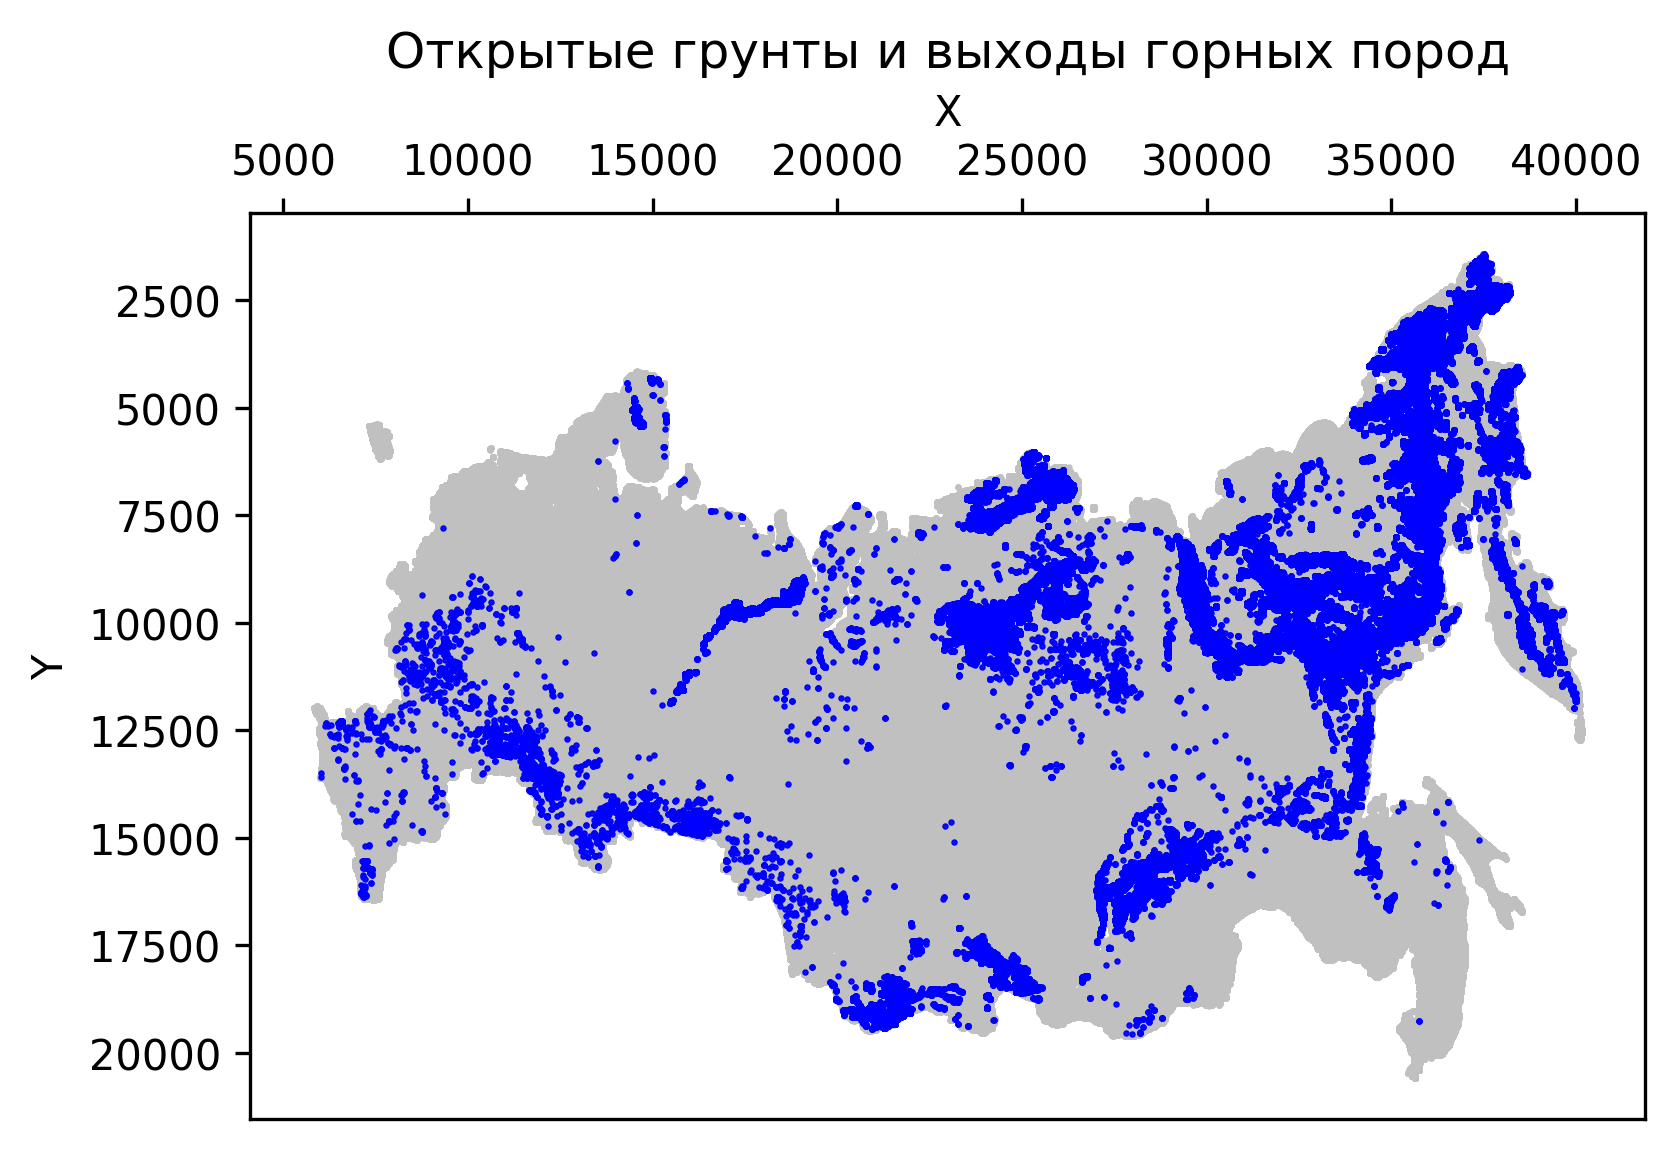
\includegraphics[]{class-13-map}
\end{figure}

\begin{figure}[H]
    \centering
    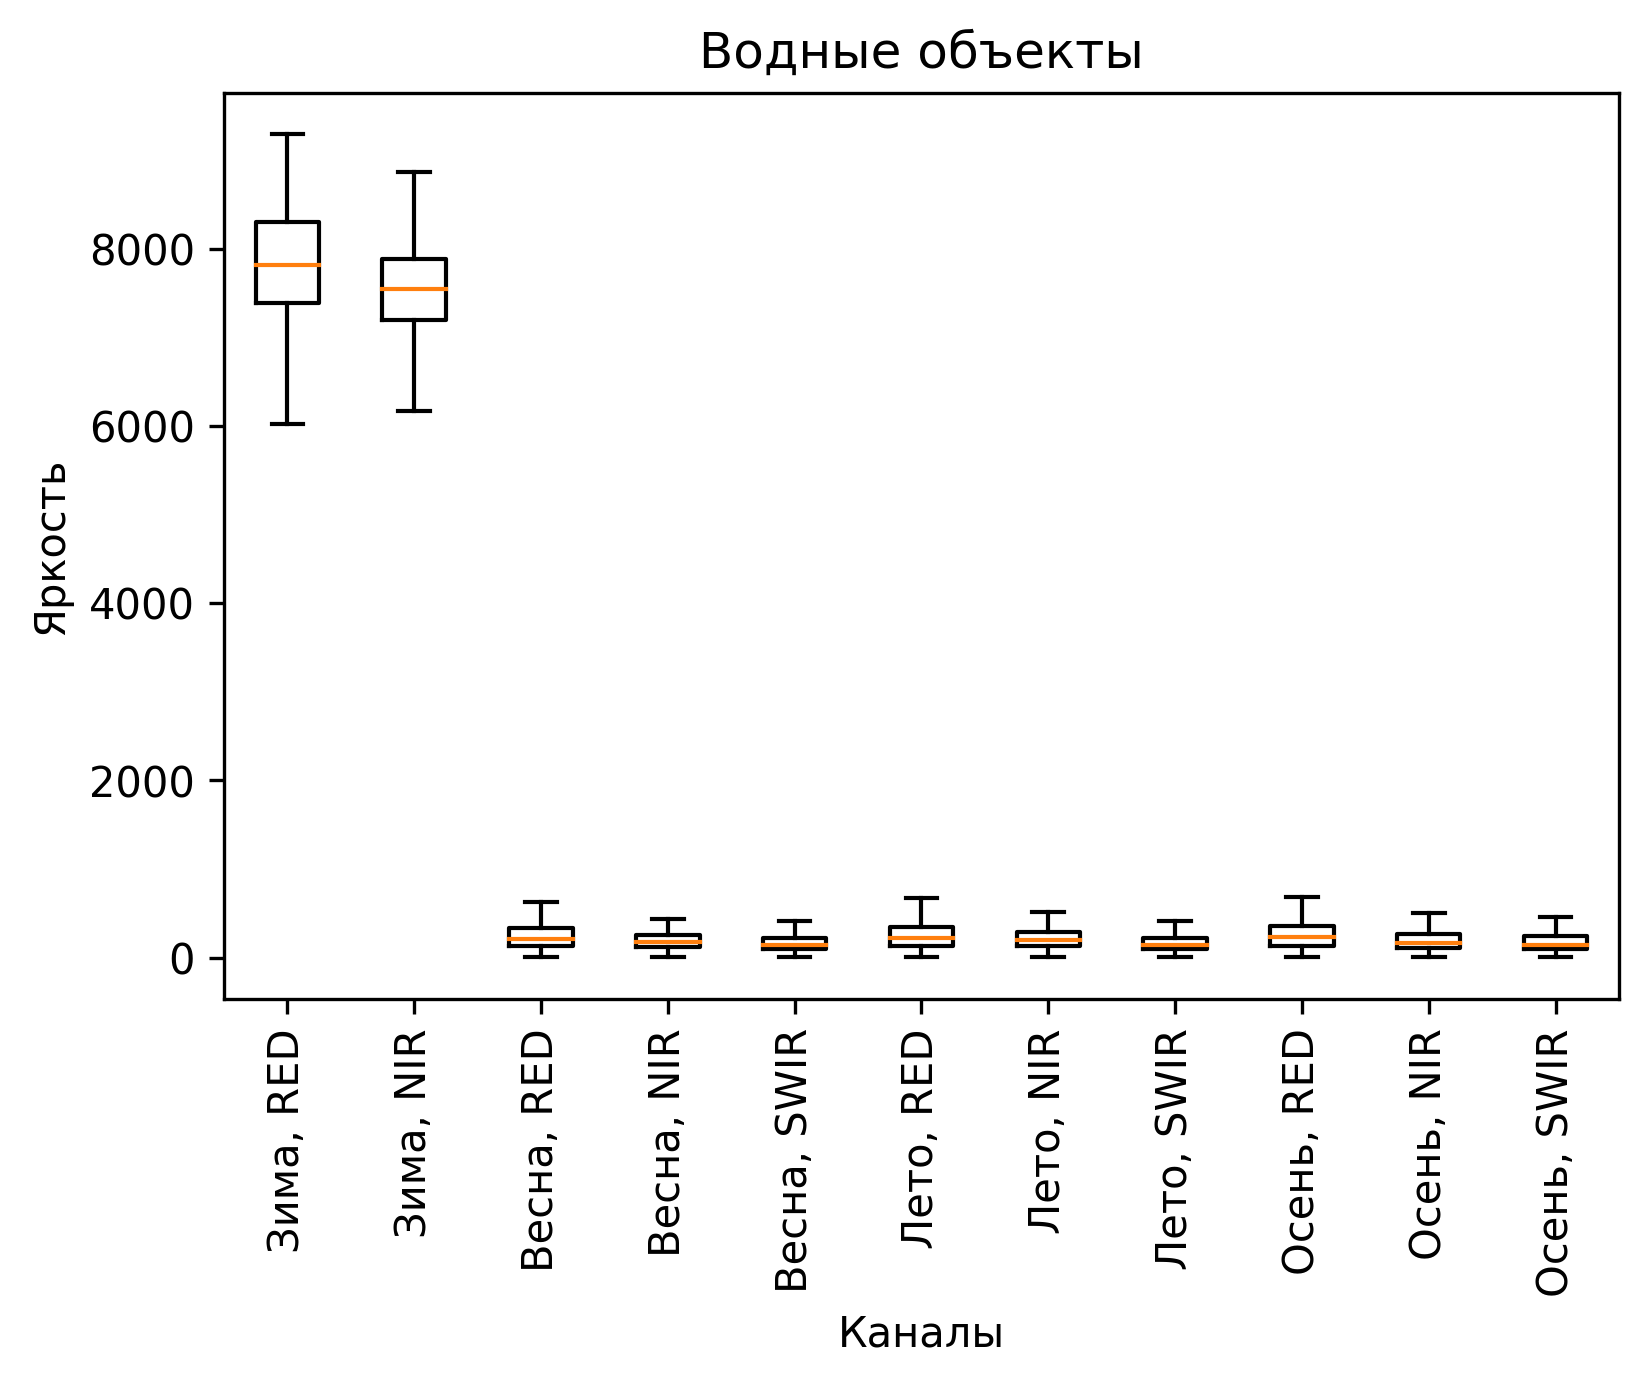
\includegraphics[]{class-20-boxplot}
    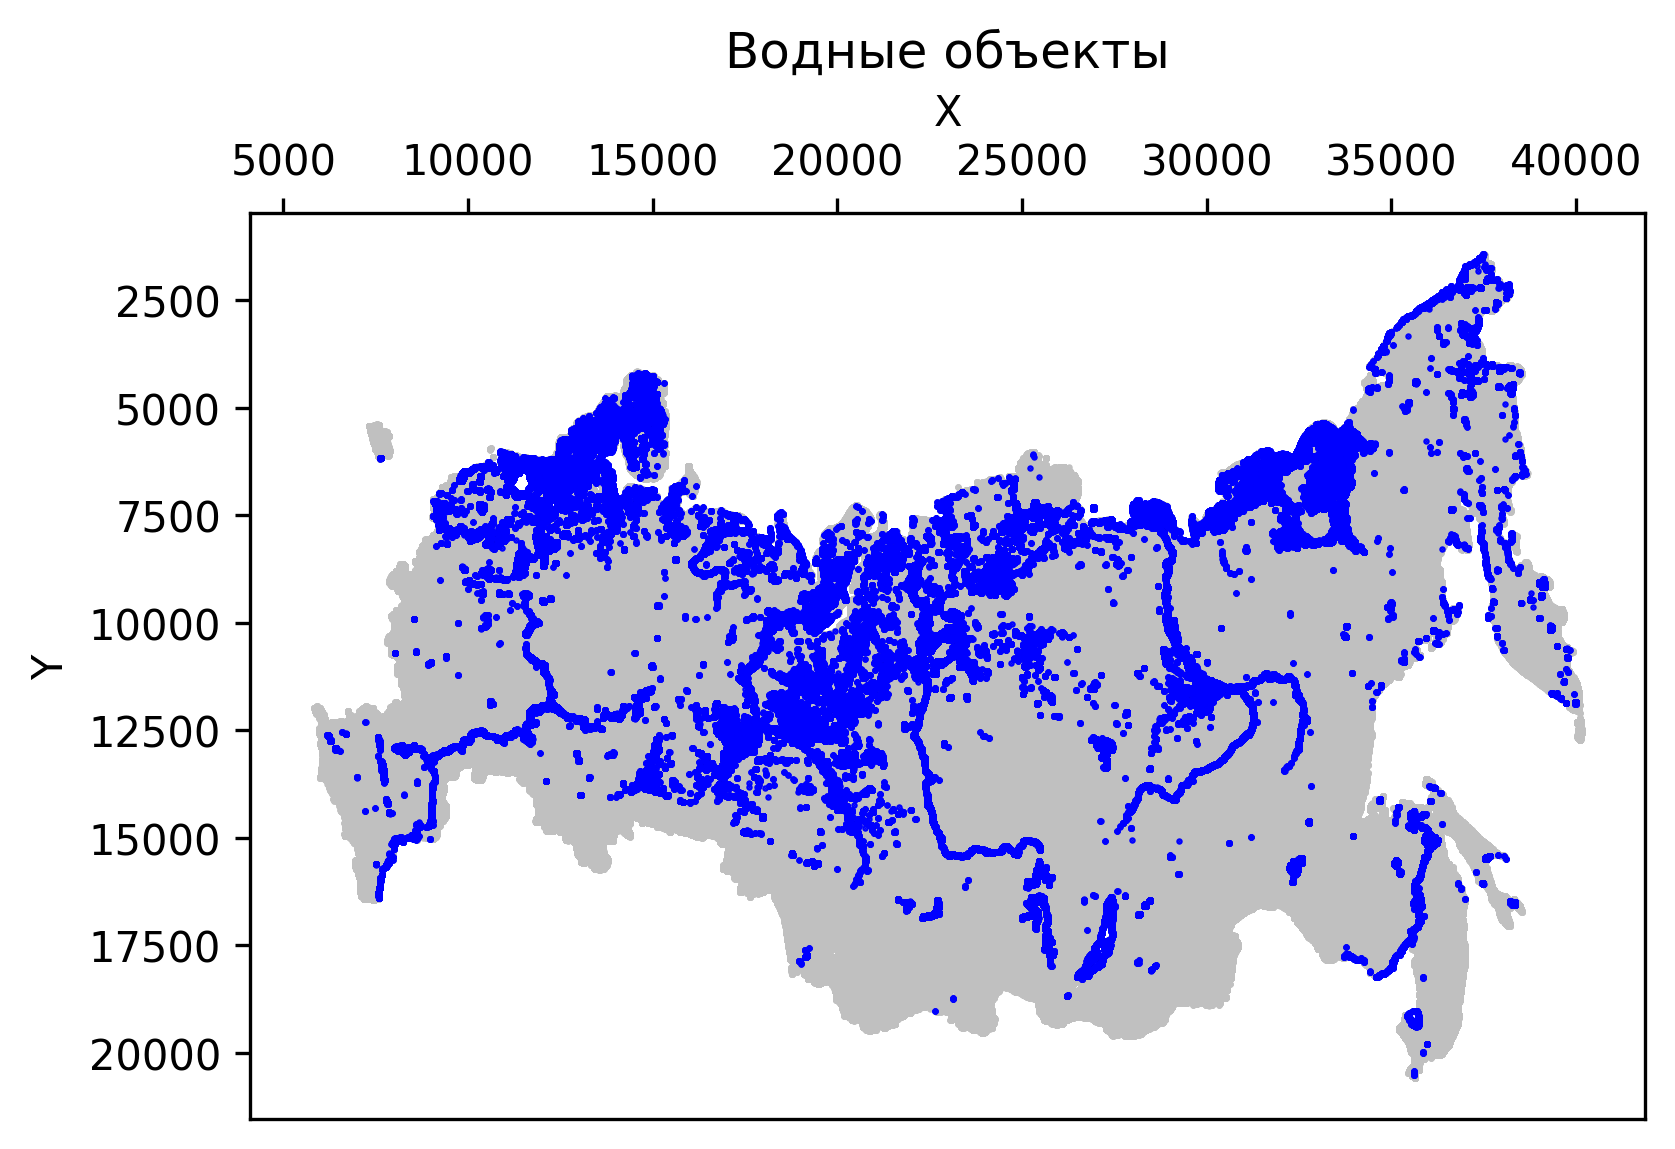
\includegraphics[]{class-20-map}
\end{figure}

\begin{figure}[H]
    \caption{Сравнение медианных значений сезонных яркостей в различных спектральных каналах по тематическим классам земного покрова, представленным в выборке}
    \centering
    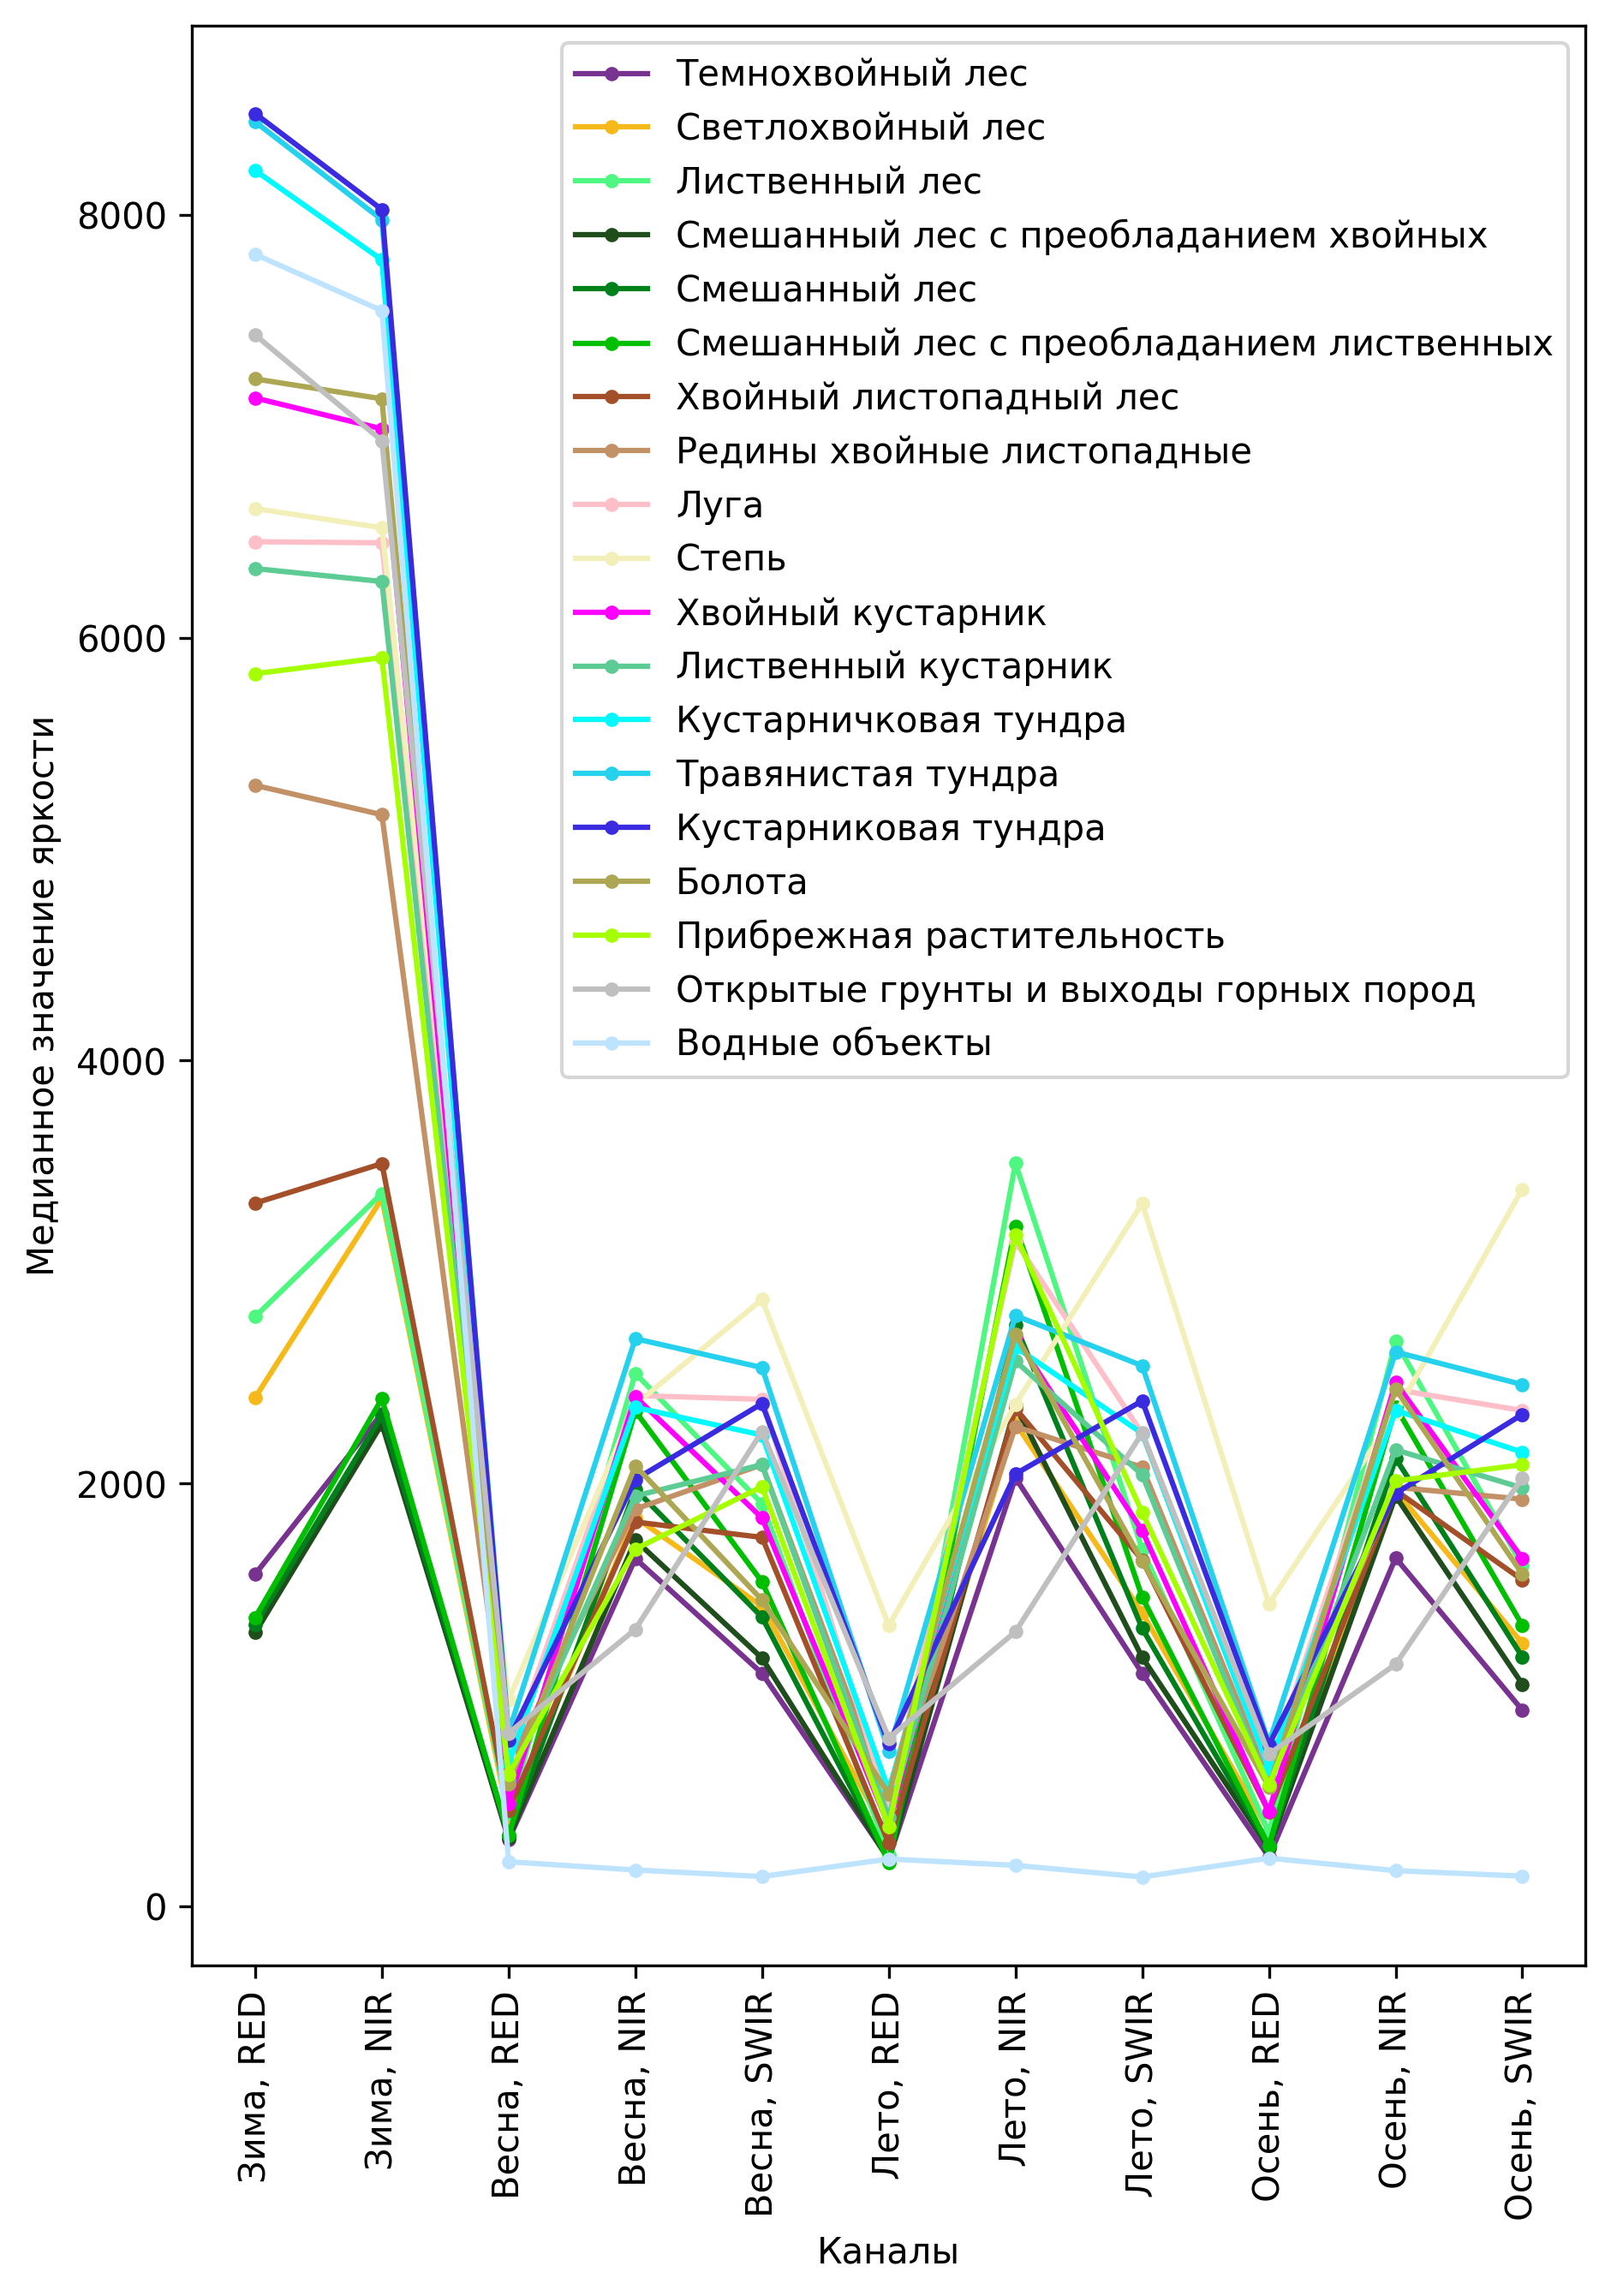
\includegraphics[]{class-comparison}
\end{figure}

\begin{landscape}
\begin{figure}[H]
    \caption{Карта земного покрова России по данным, представленным в выборке}
    \centering
    \includegraphics[scale=0.5]{full-map}
\end{figure}
\end{landscape}

\subsection{Инструменты для анализа данных}
По той причине, что для анализа данных необходимо работать с полной выборкой, содержащей 74029669 элементов, возникает проблема нехватки оперативной памяти на локальной машине при использовании классического инструмента для анализа данных --- библиотеки Pandas \cite{pandas}. В качестве более производительной альтернативы библиотеке Pandas в настоящей работе для анализа данных применяется библиотека Vaex \cite{vaex}, использующая политику нулевого копирования, параллельные и ленивые вычисления.

Для визуализации данных применяется библиотека Matplotlib \cite{matplotlib}.

\newpage

\section{Классификация земного покрова с помощью случайного леса}
\subsection{Математическая постановка задачи классификации}
Введем n-мерное пространство параметров (признаков), полученных по данным дистанционного зондирования Земли: $F=\{(f_1, f_2, ..., f_n)\}$, где $f_i$, $i=(1, ..., n)$ --- значения отдельных параметров. В нашей задаче признаками являются координаты элементов выборки и значения сезонных яркостей в различных спектральных каналах. Существует подлежащая дистанционной оценке характеристика $C$, в нашей задаче дискретная --- обозначающая типы земного покрова. Также существует неизвестная функция $A: F \to C$, которая задает отношение между множеством параметров и возможными значениями характеристики. Предположим, что для некоторого подмножества пространства параметров (обучающей выборки) $F_T \in F$ известны соответствующие им значения характеристики, что можно выразить следующим соотношением: $A_T: F_T \to C$. Также предположим, что существует некоторый метод, позволяющий на основании знаний об известных значениях характеристик и значениях параметров построить приближение к реальной функции $A: F \to C$. Обозначим этот метод $TRAIN: \{F\} \times \{F_T\} \to \{\widetilde{A}\}$. В нашей задаче функция $TRAIN$ представляет собой процесс построения классификатора по обучающей выборке. Такой способ машинного обучения называется обучением с учителем.

Важной особенностью при этом является способность обучаемой системы к обобщению, то есть к адекватному отклику на данные, выходящие за пределы имеющейся обучающей выборки. Для измерения точности ответов вводится оценочный функционал качества --- метрика.

\subsection{Численная оценка качества алгоритма}
Основой оценки качества работы алгоритма является тестовая выборка, в которой задано соответствие между элементами выборки и их классами. При наличии тестовой выборки достаточно применить классификатор к элементам данной выборки и сравнить его решения с заведомо известными экспертными решениями. Однако, для того чтобы делать выводы об относительном качестве работы различных алгоритмов или одного алгоритма с различными параметрами необходима численная метрика качества алгоритма.

Задача классификации земного покрова является задачей мультиклассовой классификации, так как целевая функция (характеристика $C$) принимает более двух значений.

Многие метрики классификации определены для бинарной классификации и требуют усреднения по классам для получения одной оценки для мультиклассовой классификации. Существует несколько подходов к решению названной проблемы: micro-, macro- и weighted-averaging.

Пусть выборка состоит из $K$ классов. Рассмотрим $K$ задач бинарной классификации, каждая из которых заключается в отделении одного класса от остальных. Для каждой из них можно вычислить различные характеристики (метрики) алгоритма. При подходе micro-averaging метрика вычисляется глобально, путем подсчета итоговых истинно-положительных, истинно-отрицательных, ложно-положительных и ложно-отрицательных результатов (независимо от классов). При подходе macro-averaging сначала вычисляется метрика для каждого класса, затем --- невзвешенное среднее по всем классам. При подходе weighted-averaging вычисляется метрика для каждого класса, а затем --- взвешенное среднее по числу представителей каждого класса.

В случае неравных по количеству представителей классов важно подбирать метрику, которая будет корректно отражать качество классификации.

Далее приведен обзор метрик, используемых для оценки качества работы алгоритмов в задачах классификации.

\subsubsection{Accuracy}
Метрика accuracy (точность) определяется долей элементов выборки, по которым классификатор принял правильное решение.
$$Accuracy = \frac{P}{N},$$
где $P$ --- количество элементов выборки по которым классификатор принял правильное решение, $N$ --- размер обучающей выборки.

Недостатком данной метрики является то, что она присваивает всем элементам выборки одинаковый вес, что может быть не корректно в случае если распределение элементов в обучающей выборке сильно смещено в сторону какого-либо одного или нескольких классов. В этом случае у классификатора есть больше информации по этим классам и соответственно в рамках этих классов он будет принимать более адекватные решения. На практике это приводит к тому, что мы имеем accuracy, допустим, 80\%, но при этом в рамках некоторого конкретного класса классификатор работает плохо, не определяя правильно и трети его представителей.

\subsubsection{Precision, Recall}
Для оценки качества работы алгоритма на каждом из классов по отдельности вводятся метрики precision (точность системы в пределах класса) и recall (полнота).

Точность системы в пределах класса --- это доля элементов выборки действительно принадлежащих данному классу относительно всех элементов которые система отнесла к этому классу.

Полнота системы --- это доля найденных классификатором элементов выборки принадлежащих классу относительно всех элементов этого класса в тестовой выборке.

Допустим, мы имеем два класса и алгоритм, предсказывающий принадлежность каждого объекта одному из классов, тогда матрица ошибок классификации будет выглядеть следующим образом:

\begin{table}[H]
    \centering
    \caption{Матрица ошибок классификации}
    \begin{tabular}{ |c|c|c| }
        \hline
        & $y=1$ & $y=0$ \\
        \hline
        $\hat{y}=1$ & True Positive (TP) & False Positive (FP) \\
        \hline
        $\hat{y}=0$ & False Negative (FN) & True Negative (TN) \\
        \hline
    \end{tabular}
\end{table}

В таблице содержится информация о том, сколько раз алгоритм принял верное и сколько раз неверное решение для элементов заданного класса (значения $y$ соответствуют экспертной оценке, значения $\hat{y}$ соответствуют оценке алгоритма).

\begin{itemize}
    \item[-] True Positive (TP) --- истинно-положительное решение;
    \item[-] True Negative (TN) --- истинно-отрицательное решение;
    \item[-] False Positive (FP) --- ложно-положительное решение;
    \item[-] False Negative (FN) --- ложно-отрицательное решение.
\end{itemize}

Тогда, точность и полнота определяются следующим образом:
$$Precision = \frac{TP}{TP+FP},$$
$$Recall = \frac{TP}{TP+FN}.$$

Precision и recall не зависят, в отличие от accuracy, от соотношения классов и потому применимы в условиях несбалансированных выборок.

\subsubsection{F-score}
На практике максимальная точность и полнота не достижимы одновременно, поэтому, хотелось бы иметь некую метрику, которая объединяла бы в себе информацию о точности и полноте алгоритма.

F-score представляет собой гармоническое среднее между точностью и полнотой. Она стремится к нулю, если точность или полнота стремятся к нулю.
$$F\mbox{-}score = 2 \frac{Precision \cdot Recall}{Precision + Recall}$$
Данная формула придает одинаковый вес точности и полноте, поэтому F-score будет уменьшаться одинаково при уменьшении и точности, и полноты.

Возможно рассчитать F-score, придав различный вес точности и полноте, если отдается приоритет одной из этих метрик при разработке алгоритма.
$$F\mbox{-}score = (\beta^2 + 1) \frac{Precision \cdot Recall}{\beta^2 Precision + Recall},$$
где $0 < \beta < 1$, если приоритет отдается точности, $\beta > 1$, если приоритет отдается полноте. При $\beta = 1$ формула сводится к предыдущей и мы получаем сбалансированную F-score (также ее называют $F_1$).

F-score является хорошим кандидатом на формальную метрику оценки качества классификатора.

\subsubsection{Confusion Matrix}
Confusion matrix (матрица ошибок, матрица неточностей) позволяет наглядно представить результаты работы классификатора в случае если количество классов относительно невелико (не более 100-150).

Матрица ошибок --- это матрица размера $N \times N$, где $N$ --- количество классов. Столбцы матрицы резервируются за экспертными решениями, а строки --- за решениями классификатора. При классификации элемента из тестовой выборки мы инкрементируем число, стоящее на пересечении строки класса который вернул классификатор и столбца класса, к которому действительно относится элемент.

При наличии матрицы ошибок точность алгоритма в пределах класса рассчитывается как отношение соответствующего этому классу диагонального элемента матрицы и суммы значений всей строки класса, полнота --- как отношение диагонального элемента матрицы и суммы значений всего столбца класса.
$$Precision_c = \frac{a_{c,c}}{\sum_{i=1}^{n} a_{c,i}},$$
$$Recall_c = \frac{a_{c,c}}{\sum_{i=1}^{n} a_{i,c}},$$
где $a_{i,j}$ --- значение $i$-го по строке, $j$-го по столбцу элемента матрицы, $c$ --- индекс класса, $n$ --- количество классов.

Результирующая точность классификатора рассчитывается как арифметическое среднее его точности по всем классам, аналогично рассчитывается полнота, данный подход называется macro-averaging.

\subsubsection{Receiver Operating Characteristic Curve, Area Under Receiver Operating Characteristic Curve}
Receiver operating characteristic curve (ROC, кривая ошибок) является одним из способов оценить модель в целом и представляет из себя линию от точки (0, 0) до точки (1, 1) в координатах True Positive Rate (TPR) и False Positive Rate (FPR):
$$TPR = \frac{TP}{TP+FN},$$
$$FPR = \frac{FP}{FP+TN},$$
где TPR --- полнота (доля элементов класса 1, которые верно классифицированы алгоритмом), FPR --- доля элементов класса 0, которые неверно классифицированы алгоритмом.

Area Under Receiver Operating Characteristic Curve (AUC ROC, площадь под кривой ошибок) является агрегированной характеристикой качества классификации, не зависящей от соотношения цен ошибок. Чем больше значение AUC ROC, тем лучше модель классификации, кроме этого, важной является крутизна кривой --- мы максимизируем TPR, минимизируя FPR, а значит, кривая должна стремиться к точке (0, 1). В идеальном случае, когда классификатор не делает ошибок ($FPR = 0$, $TPR = 1$) мы получим площадь под кривой, равную 1; в случае, когда классификатор случайно выдает метки классов, AUC ROC будет стремиться к 0,5, так как классификатор будет выдавать одинаковое количество TP и FP.

Критерий AUC ROC устойчив к несбалансированным классам.

\subsubsection{Out-of-Bag Error}
Out-of-bag error (OOB) --- это метод измерения ошибки предсказания случайных лесов и других моделей машинного обучения, использующих bagging.

Bagging --- технология классификации, использующая композиции алгоритмов (для модели случайного леса это ансамбль решающих деревьев), каждый из которых обучается независимо. Классификаторы не исправляют ошибки друг друга, а компенсируют их при голосовании. Bagging позволяет снизить процент ошибки классификации в случае, когда высока дисперсия ошибки базового метода.

Суть метода измерения ошибки OOB заключается в том, что при использовании технологии bagging каждый классификатор ансамбля обучается не на полной выборке, а на ее части, оставшаяся же часть выборки используется для оценки данного классификатора. Таким образом производится оценка каждого решающего дерева случайного леса, что позволяет получить характеристику качества работы случайного леса в целом.

Ошибка OOB может быть использована для валидации, что позволит подобрать оптимальное количество деревьев случайного леса.

\subsection{Случайный лес}
В настоящей работе классификация типов земного покрова по данным дистанционного зондирования Земли производится с помощью модели случайного леса. Используется реализация случайного леса, предоставляемая библиотекой Scikit-learn \cite{sklearn}.

\subsubsection{Модель случайного леса}
Случайный лес --- алгоритм машинного обучения, заключающийся в использовании ансамбля решающих деревьев.

Пусть обучающая выборка состоит из $N$ элементов, размерность пространства признаков равна $M$, и задан параметр $m$ (в задачах классификации обычно $m \approx \sqrt{M}$) как неполное количество признаков для обучения.

Построение деревьев ансамбля (bagging) производится следующим образом:
\begin{enumerate}
    \item Сгенерируем случайную повторную подвыборку размером $N$ из обучающей выборки. Некоторые элементы попадут в неё два или более раза, тогда как в среднем $N(1-\frac{1}{N})^N$ (при больших $N$ примерно $\frac{N}{e}$, где $e$ --- основание натурального логарифма) образцов оказываются не вошедними в набор или неотобранными (out-of-bag).
    \item Построим решающее дерево, классифицирующее элементы данной подвыборки, причём в ходе создания очередного узла дерева будем выбирать набор признаков, на основе которых производится разбиение (не из всех $M$ признаков, а лишь из $m$ случайно выбранных).
    \item Дерево строится до полного исчерпания подвыборки и не подвергается процедуре прунинга (отсечения ветвей).
\end{enumerate}

Классификация элементов проводится путём голосования: каждое дерево ансамбля относит классифицируемый элемент к одному из классов, а побеждает класс, за который проголосовало наибольшее число деревьев.

Увеличение количества деревьев в ансамбле позволяет повысить качество классификации. Однако, при увеличении числа деревьев возрастает так же время обучения и работы случайного леса.

\subsubsection{Предпосылки использования случайного леса}
Модель случайного леса успешно справляется с классификацией данных высокой размерности, оставаясь при этом быстрой и нечувствительной к переобучению. Оценка значимости признаков, обеспечиваемая классификатором, может быть использована для уменьшения числа признаков в выборке, для определения наиболее релевантных данных дистанционного зондирования, а также для выбора наиболее подходящих сезонов и спектральных каналов для классификации определенных типов земного покрова, что показано в работе \cite{random-forest-in-remote-sensing}.

\subsubsection{Обучение случайного леса и оценка качества классификации}
Для обучения случайного леса набор данных разделен на обучающую (2000000 элементов) и тестовую выборки (72029669 элементов). Затем обучающая выборка разделена на непосредственно обучающую (200000 элементов) и валидационную (1800000 элементов) выборки.

Предварительная обработка данных перед обучением модели не осуществляется, так как она не влияет на качество работы случайного леса и данные не содержат пропущенных значений.
% Proof: https://stats.stackexchange.com/questions/172842/best-practices-with-data-wrangling-before-running-random-forest-predictions

Произведено обучение случайного леса с гиперпараметрами по умолчанию и получены предсказания типов земного покрова для валидационной выборки. Ниже приведены оценки качества классификации валидационной выборки обученной моделью случайного леса с гиперпараметрами по умолчанию:
\begin{itemize}
    \item[] $Accuracy = 0.95334,$
    \item[] $F_1\mbox{-}score = 0.95249$ (при взвешенном усреднении),
    \item[] $Out\mbox{-}of\mbox{-}bag\ error = 0.95189.$
\end{itemize}

\begin{figure}[H]
    \caption{Матрица ошибок классификации случайного леса с гиперпараметрами по умолчанию}
    \centering
    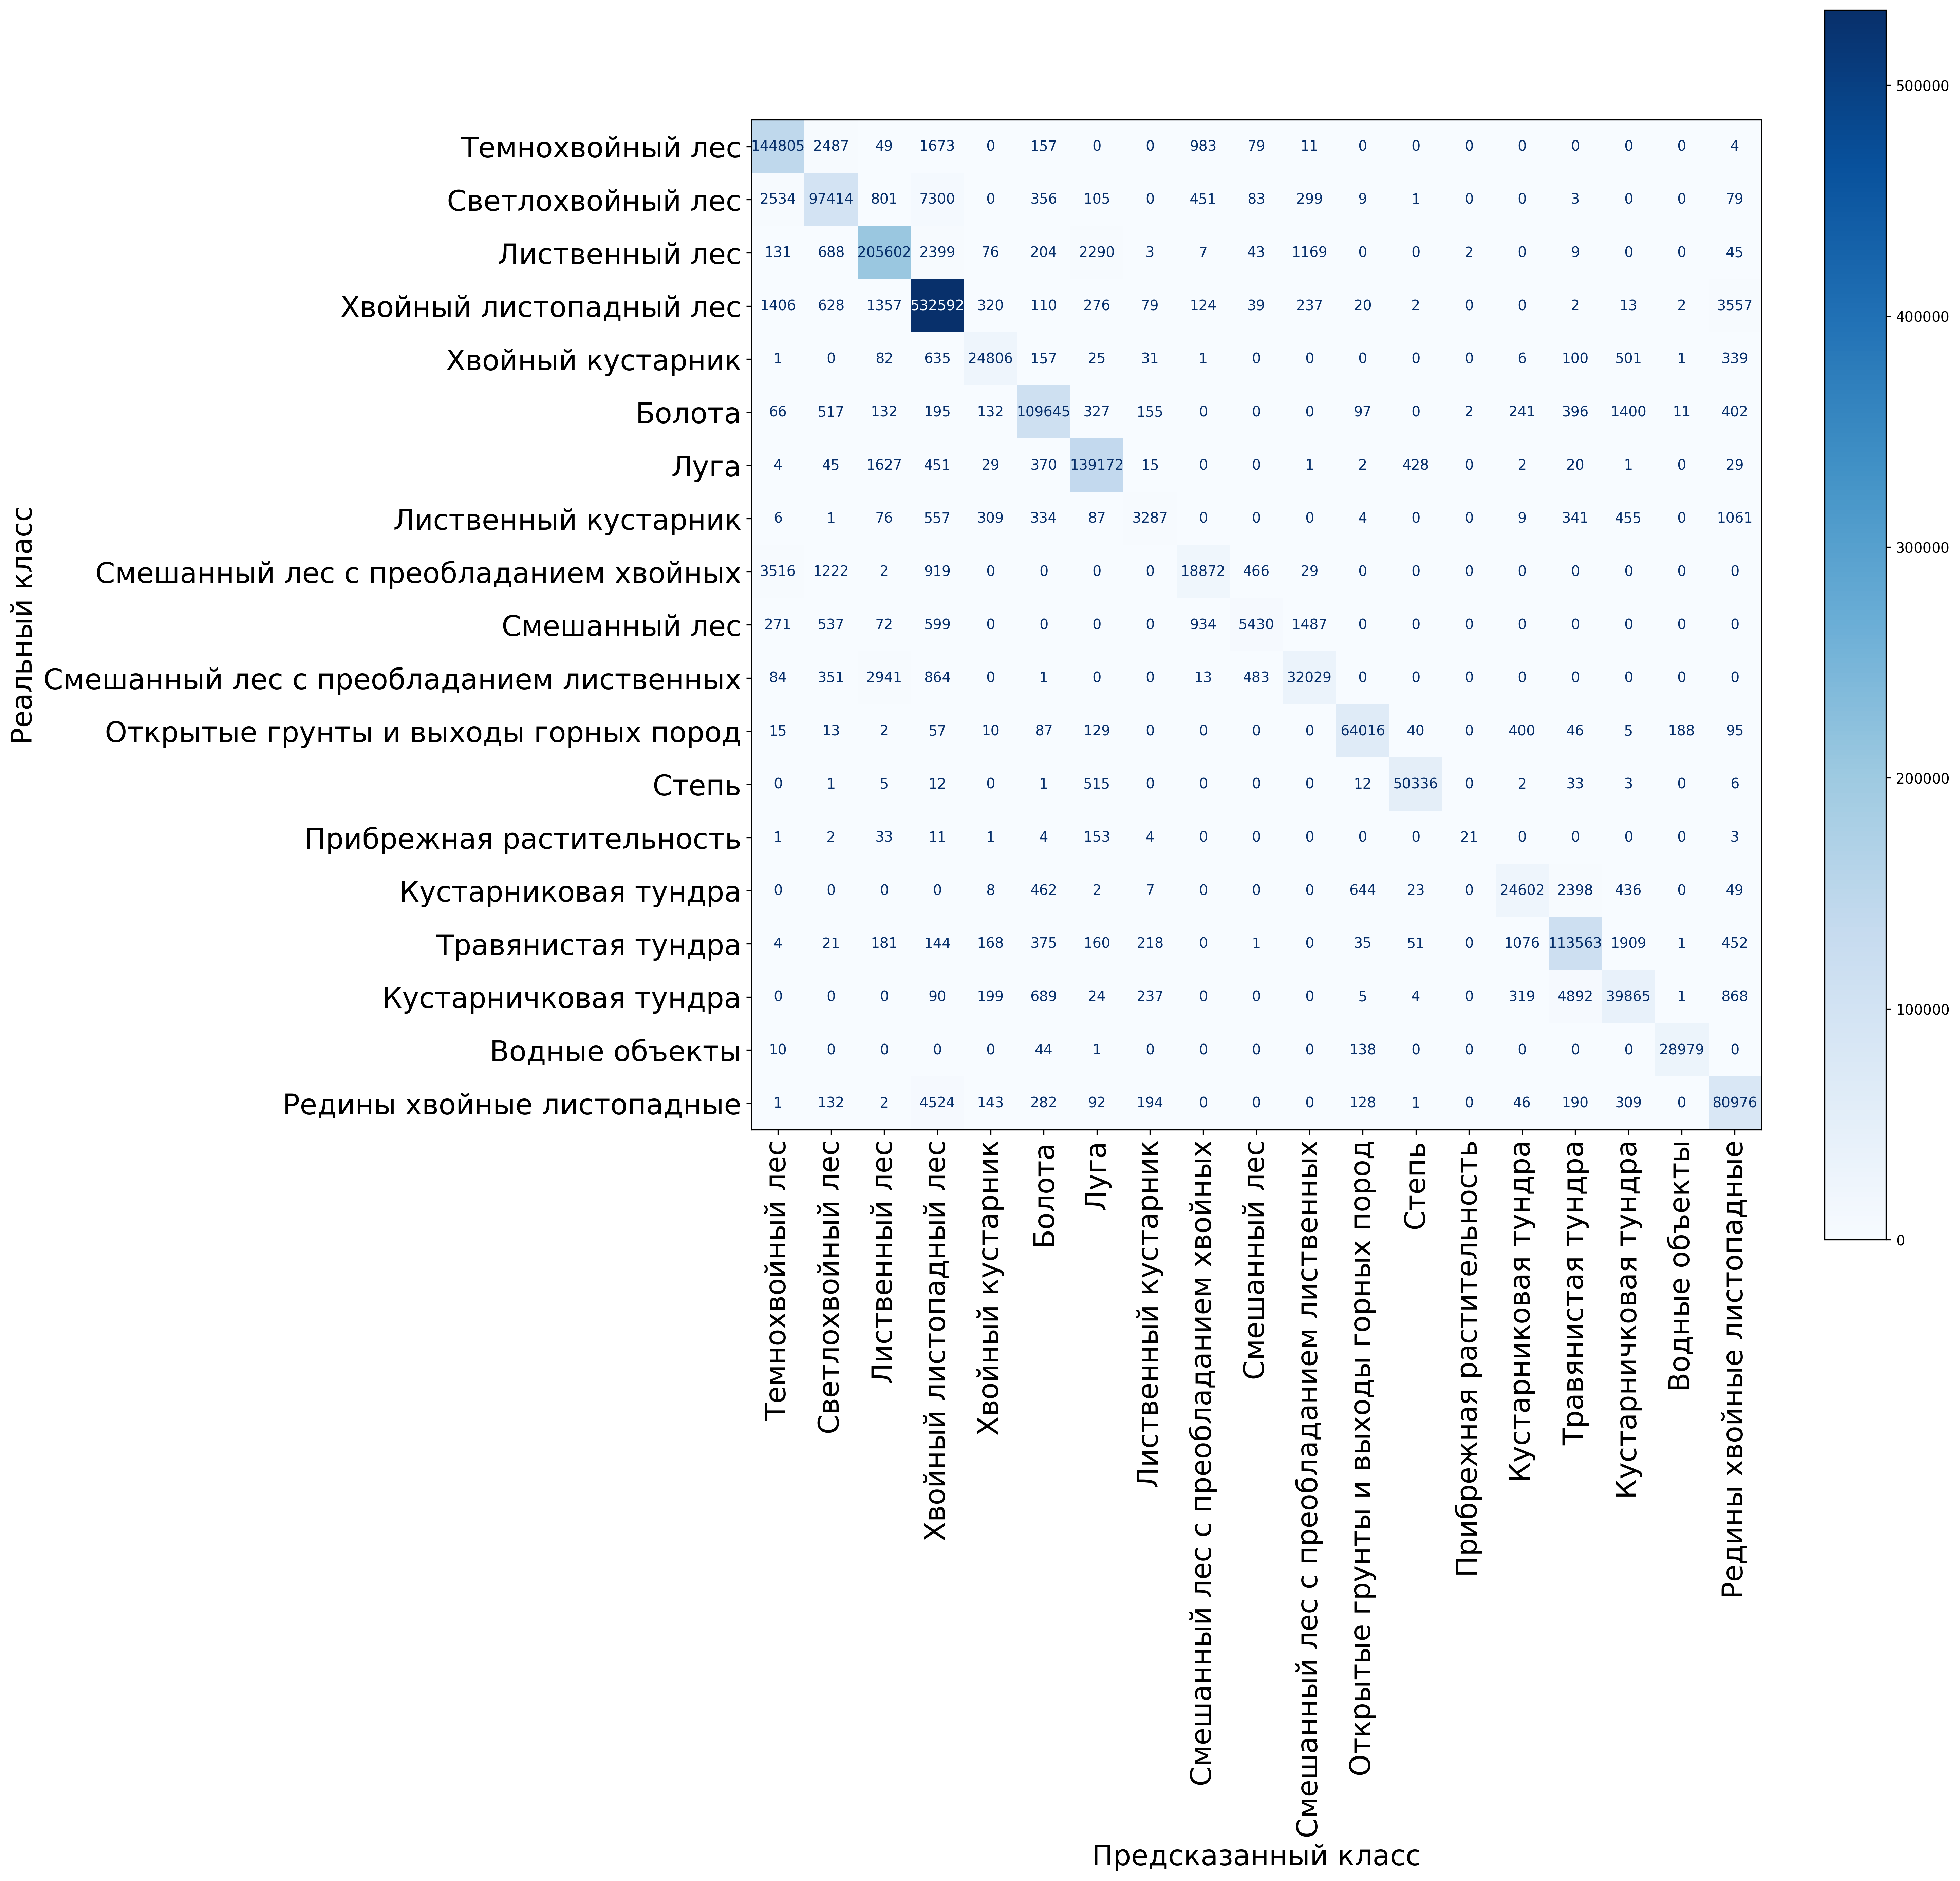
\includegraphics[scale=0.33]{confusion-matrix-1}
\end{figure}

\begin{figure}[H]
    \caption{Нормированная по строкам матрица неточностей классификации случайного леса с гиперпараметрами по умолчанию}
    \centering
    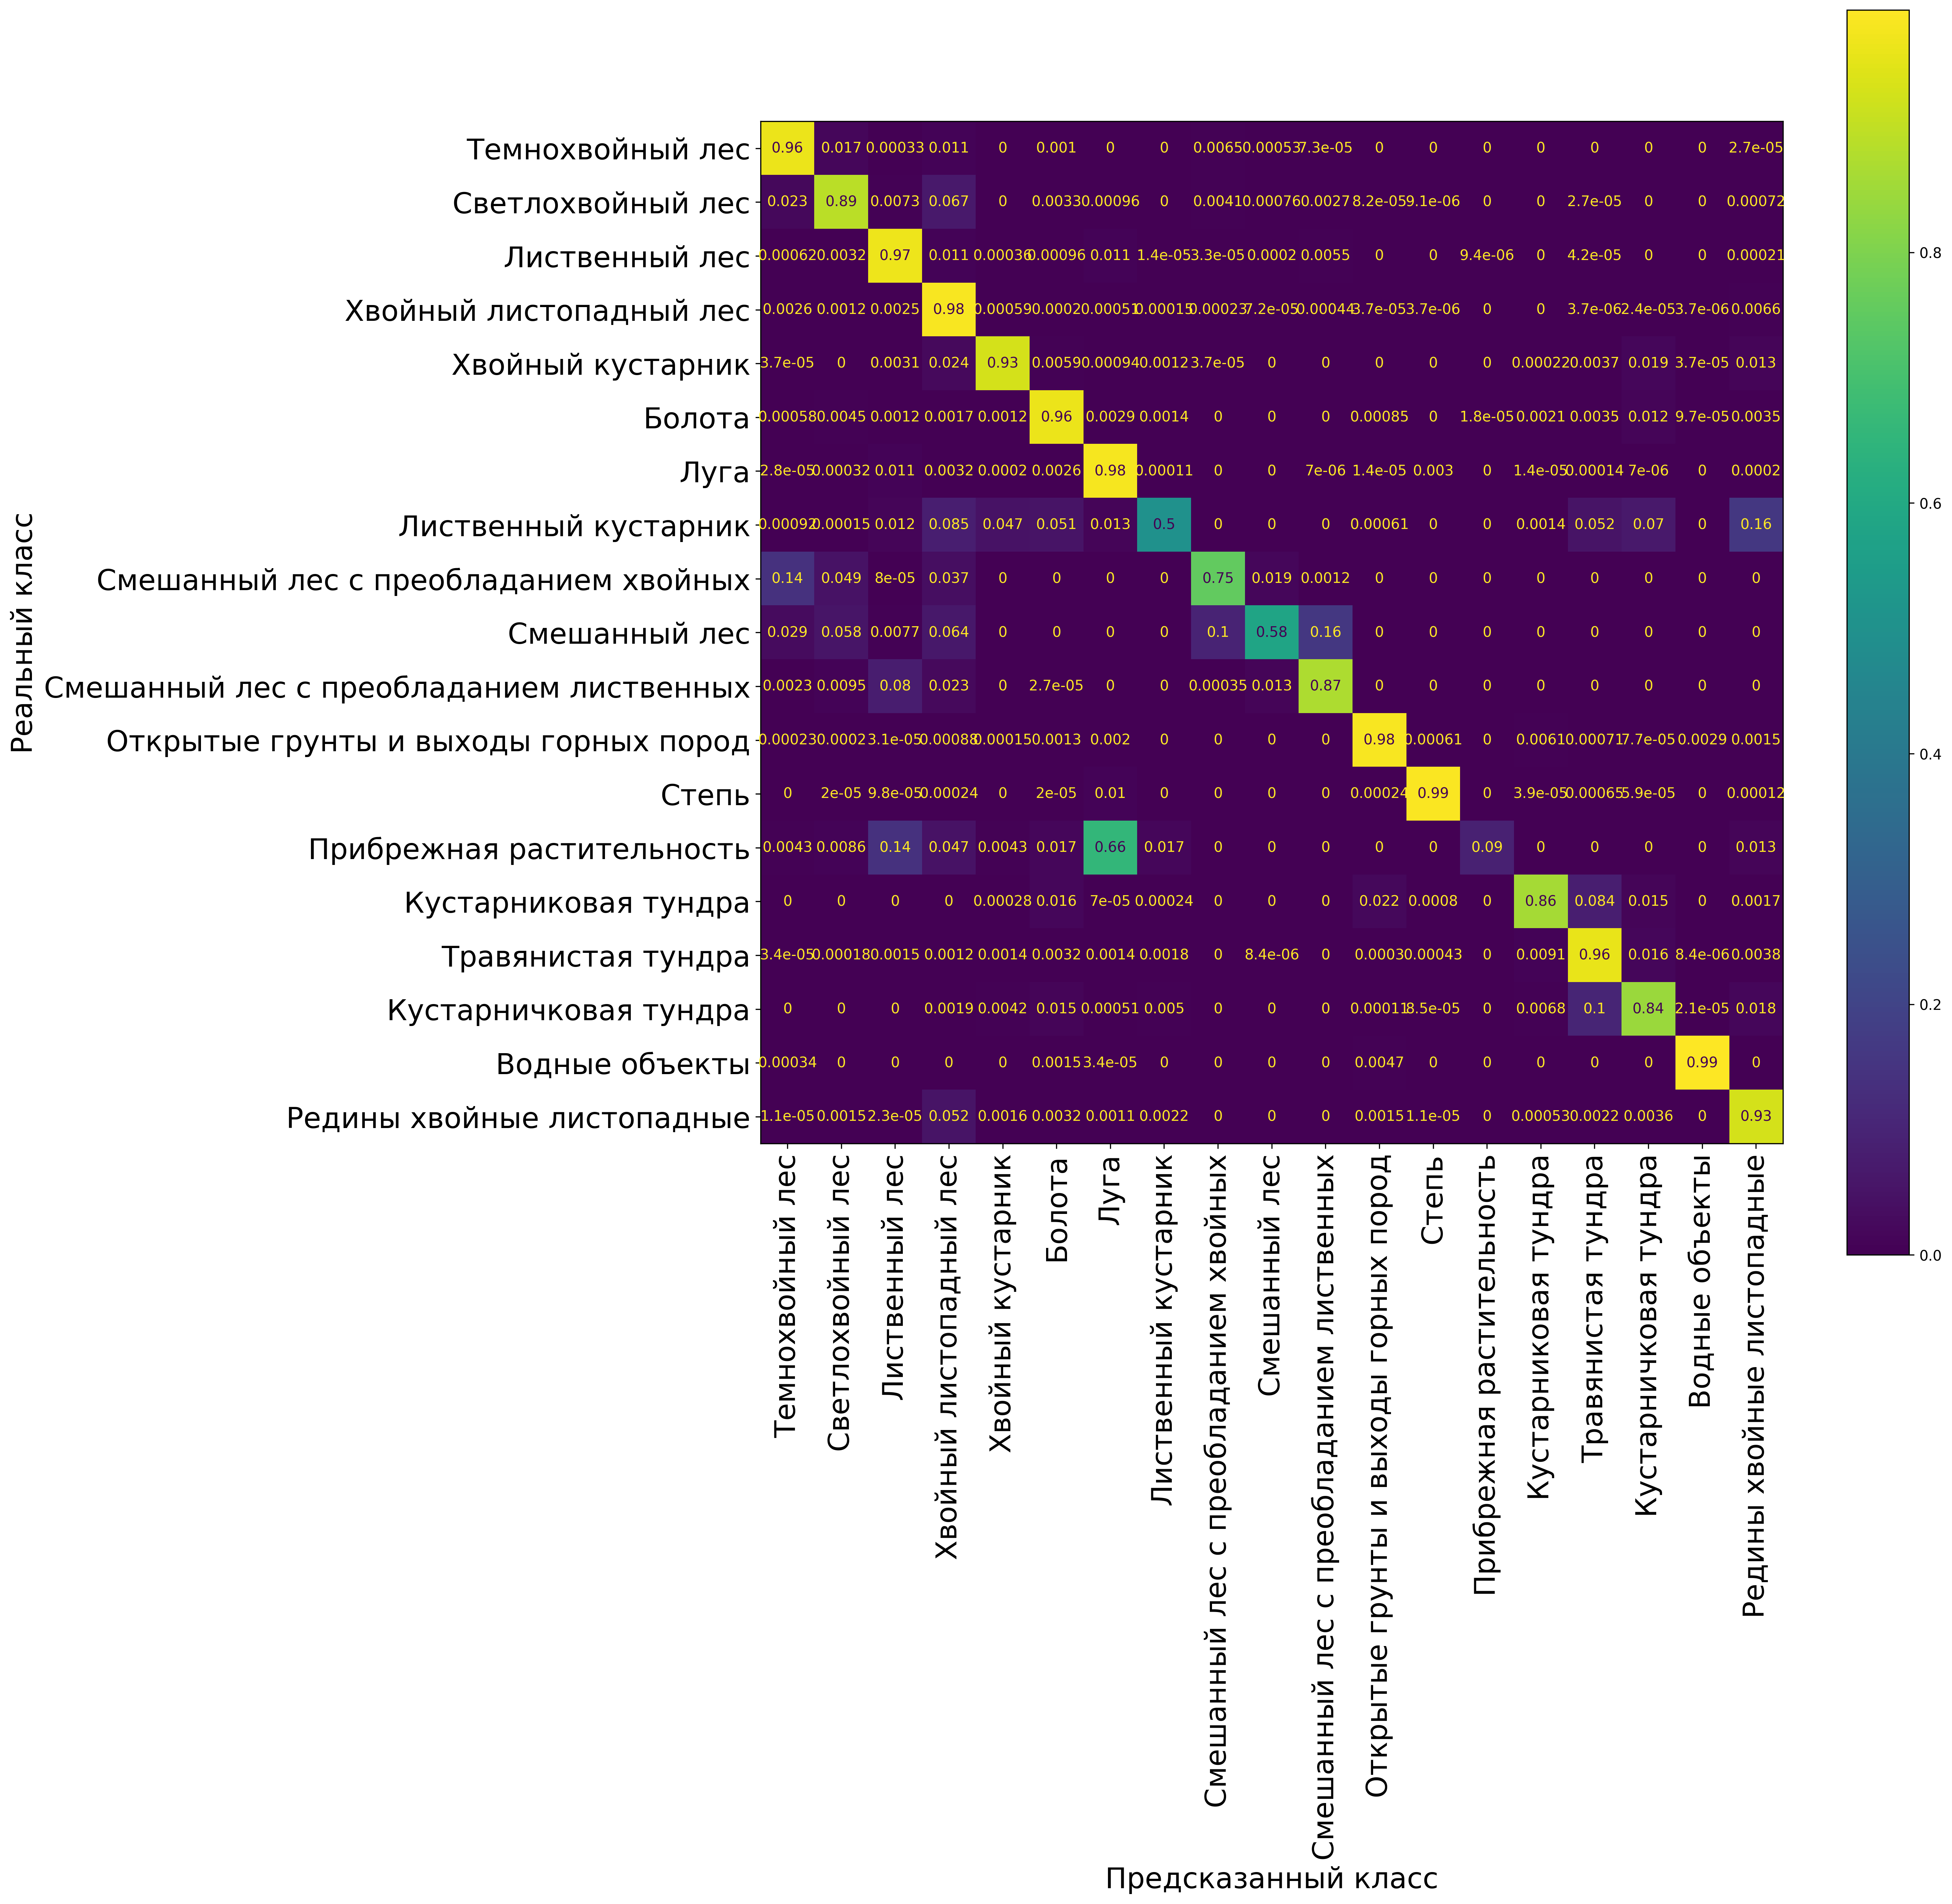
\includegraphics[scale=0.33]{confusion-matrix-2}
\end{figure}

\subsubsection{Оптимизация гиперпараметров алгоритма}
Осуществлён подбор оптимальных гиперпараметров (количества деревьев, числа признаков для выбора расщепления, максимальной глубины дерева, критерия расщепления) модели случайного леса для данной выборки.

Оптимальное количество деревьев --- 600, число признаков для выбора расщепления --- квадратный корень количества признаков, максимальная глубина дерева --- 20, критерий расщепления --- энтропийный.

Однако, качество классификации моделью с оптимальными гиперпараметрами возрастает крайне несущественно ($F_1\mbox{-}score = 0.95342$ (при взвешенном усреднении), что лишь на тысячные доли превышает значение $F_1\mbox{-}score = 0.95249$ модели с гиперпараметрами по умолчанию). При этом время обучения модели ощутимо возрастает (в основном из-за увеличения количества и глубины деревьев). Поэтому принято решение использовать для классификации модель с частично оптимальными гиперпараметрами (число признаков для выбора расщепления --- квадратный корень количества признаков, критерий расщепления --- энтропийный), для которой $F_1\mbox{-}score = 0.95341$.

\subsubsection{Проверка случайного леса на полной тестовой выборке}
Произведено обучение случайного леса с выбранными гиперпараметрами на полной обучающей выборке (2000000 элементов) и получены предсказания типов земного покрова для полной тестовой выборки (72029669 элементов). Ниже приведены оценки качества классификации полной тестовой выборки обученной моделью случайного леса с выбранными гиперпараметрами:
\begin{itemize}
    \item[] $Accuracy = 0.97214,$
    \item[] $F_1\mbox{-}score = 0.97185$ (при взвешенном усреднении),
    \item[] $Out\mbox{-}of\mbox{-}bag\ error = 0.97118.$
\end{itemize}

\begin{figure}[H]
    \caption{Матрица ошибок классификации случайного леса с выбранными гиперпараметрами}
    \centering
    \includegraphics[scale=0.27]{confusion-matrix-3}
\end{figure}

\begin{figure}[H]
    \caption{Нормированная по строкам матрица неточностей классификации случайного леса с выбранными гиперпараметрами}
    \centering
    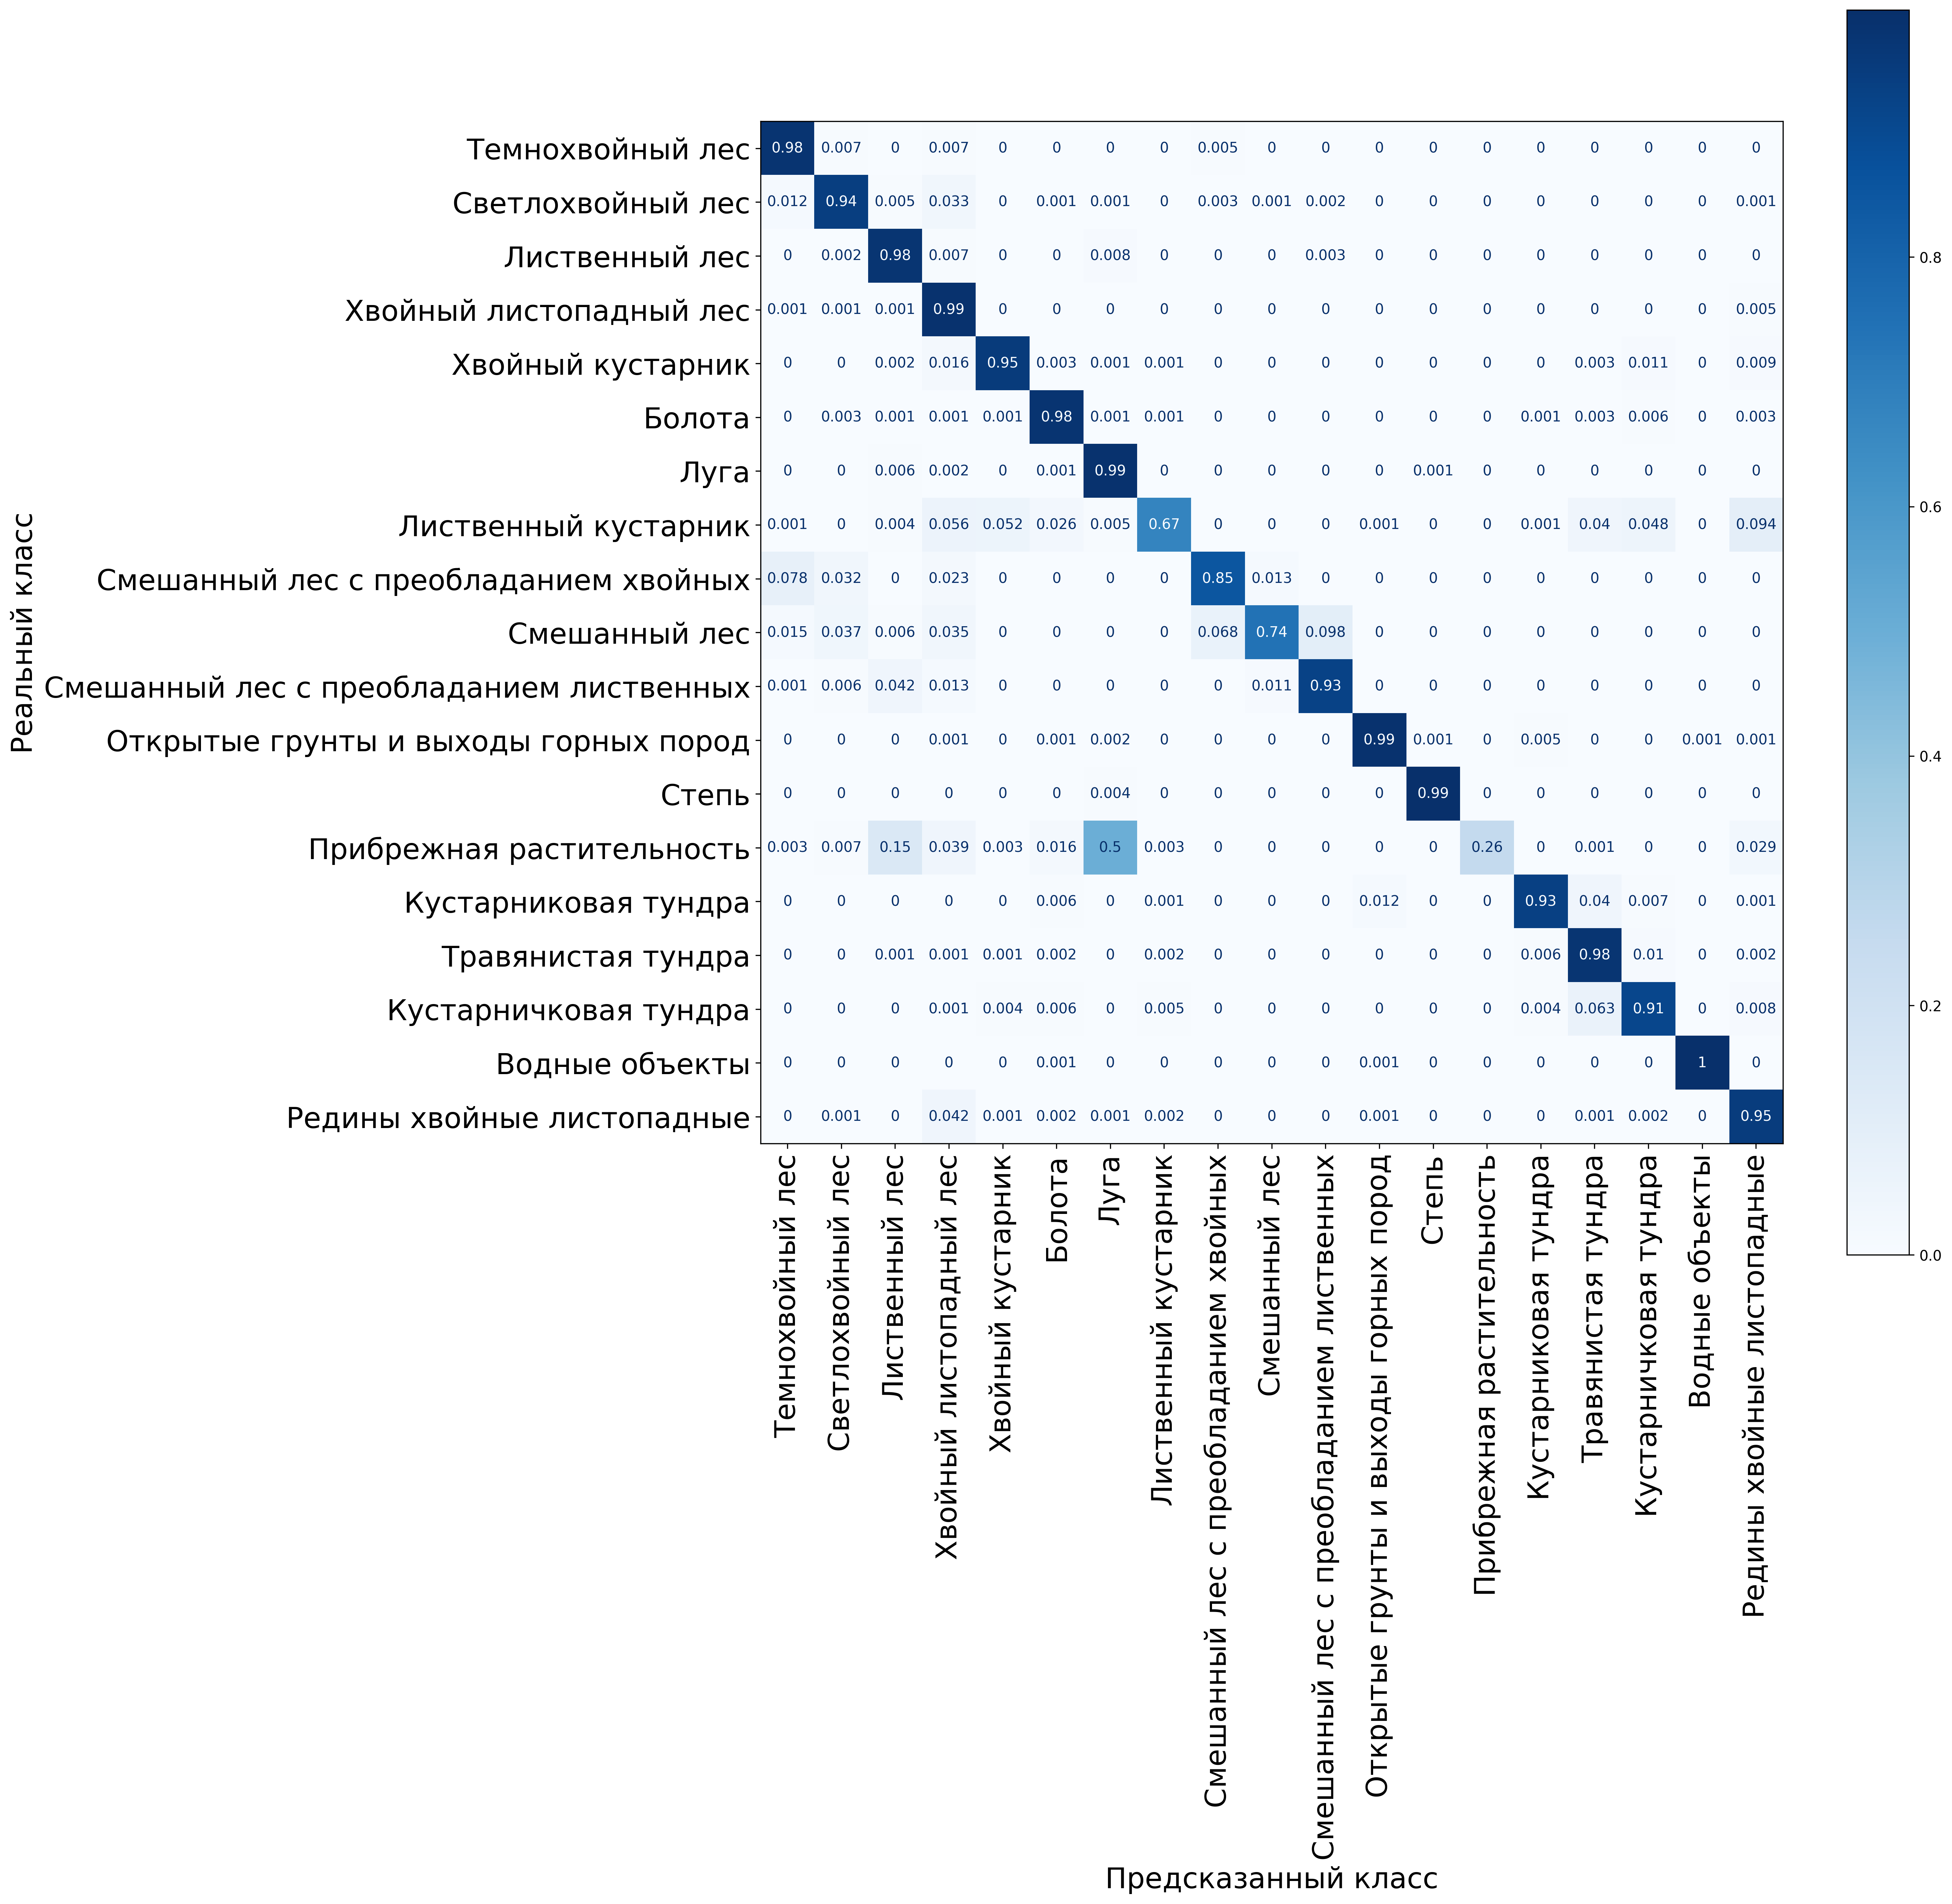
\includegraphics[scale=0.33]{confusion-matrix-4}
\end{figure}
\newpage

\section{Оценка значимости признаков}
% Методы оценки значимости признаков

% Уменьшать количество признаков --- оценивать влияние на качество классификации и время обучения
\newpage

% \section{Применение модели случайного леса к полному набору данных}
% Применение результатов исследования к полному набору данных, confusion matrix
% \newpage

% \section{Применение модели случайного леса к карте земного покрова}
% Получить табличные данные из изображений (GDAL)

% Применить модель к полученным данным, применима ли модель?
% \newpage

\section{Заключение}
\newpage

\section{Литература}
\begingroup
\renewcommand{\section}[2]{}
\begin{thebibliography}{20}
    \bibitem{land-cover-mapping-monograph}
    \textit{Барталев С.А., Егоров В.А., Жарко В.О., Лупян Е.А., Плотников Д.Е., Хвостиков С.А., Шабанов Н.В.} Спутниковое картографирование растительного покрова России // ИКИ РАН. 2016. C. 93-110.

    \bibitem{land-cover-mapping-article}
    \textit{Барталев С.А., Егоров В.А., Жарко В.О., Лупян Е.А., Плотников Д.Е., Хвостиков С.А.} Состояние и перспективы развития методов спутникового картографирования растительного покрова России // Современные проблемы дистанционного зондирования Земли из космоса. 2015. Т. 12. № 5. С. 203-221.

    \bibitem{random-forest-in-remote-sensing}
    \textit{Belgiu M., Drăguţ L.} Random forest in remote sensing: A review of applications and future
    directions // ISPRS Journal of Photogrammetry and Remote Sensing. 2016. No. 114. pp. 24-31.
    
    \bibitem{python}
    Документация языка Python\\
    \url{https://docs.python.org/3/}

    \bibitem{pandas}
    Документация библиотеки Pandas\\
    \url{https://pandas.pydata.org/docs/}

    \bibitem{vaex}
    Документация библиотеки Vaex\\
    \url{https://vaex.io/docs/}

    \bibitem{matplotlib}
    Документация библиотеки Matplotlib\\
    \url{https://matplotlib.org/stable/}

    \bibitem{sklearn}
    Документация библиотеки Scikit-learn\\
    \url{https://scikit-learn.org/stable/}
\end{thebibliography}
\endgroup
\newpage

\section{Приложения}
\begin{itemize}
    \item[\ExternalLink] Репозиторий проекта на GitHub\\
    \url{https://github.com/eugeuie/masters-term-paper}
\end{itemize}
\newpage

\end{document}
